% ============================================================
%  SmartPM — Rapport PFE TEK-UP / Capgemini
%  Compilez avec: pdflatex main.tex (x2) puis biber main
% ============================================================
\documentclass[12pt, a4paper, oneside]{report}

% ── Packages ─────────────────────────────────────────────
\usepackage[utf8]{inputenc}
\usepackage[T1]{fontenc}
\usepackage[french]{babel}
\usepackage{lmodern}

% Mise en page
\usepackage[
  top=2.5cm, bottom=2.5cm,
  left=3cm,  right=2.5cm
]{geometry}
\usepackage{setspace}
\onehalfspacing

% Couleurs & graphiques
\usepackage[table,xcdraw]{xcolor}
\usepackage{graphicx}
\usepackage{float}
\usepackage{wrapfig}
\usepackage{subcaption}
\usepackage{tikz}

% Tableaux
\usepackage{booktabs}
\usepackage{tabularx}
\usepackage{multirow}
\usepackage{longtable}
\usepackage{array}
\usepackage{colortbl}

% En-têtes et pieds de page
\usepackage{fancyhdr}
\usepackage{emptypage}

% Liens hypertexte
\usepackage[
  colorlinks=true,
  linkcolor=blue!60!black,
  urlcolor=blue!70!black,
  citecolor=green!50!black
]{hyperref}

% Code source
\usepackage{listings}
\usepackage{minted}

% Listes d'abréviations
\usepackage[acronym, toc]{glossaries}

% Bibliographie
\usepackage[backend=biber, style=numeric, sorting=none]{biblatex}
\addbibresource{bibliography.bib}

% Divers
\usepackage{amsmath}
\usepackage{amssymb}
\usepackage{enumitem}
\usepackage{pifont}
\usepackage{fontawesome5}
\usepackage{mdframed}
\usepackage{tcolorbox}
\tcbuselibrary{skins, breakable}
\usepackage{titlesec}
\usepackage{titletoc}

% ── Couleurs du projet ────────────────────────────────────
\definecolor{primaryblue}{RGB}{0, 84, 166}      % Bleu TEK-UP / Capgemini
\definecolor{accentgold}{RGB}{255, 193, 7}       % Or accent
\definecolor{lightgray}{RGB}{245, 245, 245}
\definecolor{darkgray}{RGB}{64, 64, 64}
\definecolor{successgreen}{RGB}{40, 167, 69}
\definecolor{tablehead}{RGB}{0, 84, 166}

% ── Style des chapitres ───────────────────────────────────
\titleformat{\chapter}[display]
  {\normalfont\huge\bfseries\color{primaryblue}}
  {\chaptertitlename\ \thechapter}{20pt}{\Huge}

\titleformat{\section}
  {\normalfont\Large\bfseries\color{primaryblue}}
  {\thesection}{1em}{}

\titleformat{\subsection}
  {\normalfont\large\bfseries\color{darkgray}}
  {\thesubsection}{1em}{}

\titleformat{\subsubsection}
  {\normalfont\normalsize\bfseries\color{darkgray}}
  {\thesubsubsection}{1em}{}

% ── Style des en-têtes ────────────────────────────────────
\pagestyle{fancy}
\fancyhf{}
\fancyhead[L]{\small\color{darkgray}\leftmark}
\fancyfoot[C]{\thepage}
\renewcommand{\headrulewidth}{0.4pt}
\renewcommand{\footrulewidth}{0pt}

% ── Boîtes personnalisées ─────────────────────────────────
\newtcolorbox{infobox}[1][]{
  colback=blue!5!white, colframe=primaryblue,
  title=#1, fonttitle=\bfseries\color{white},
  colbacktitle=primaryblue, breakable
}

\newtcolorbox{notebox}{
  colback=accentgold!10!white, colframe=accentgold!80!black,
  leftrule=3pt, toprule=0pt, bottomrule=0pt, rightrule=0pt,
  breakable
}

% ── Commandes utiles ──────────────────────────────────────
\newcommand{\placeholder}[1]{%
  \begin{center}
    \begin{tcolorbox}[
      colback=gray!10, colframe=gray!50,
      width=0.9\textwidth, halign=center,
      height=6cm, valign=center
    ]
      \Large\color{gray}\faImage\\[0.5em]
      \normalsize\textit{#1}
    \end{tcolorbox}
  \end{center}
}

% ── Glossaire / Abréviations ──────────────────────────────
\makeglossaries

% ── Document ──────────────────────────────────────────────
\begin{document}

% Pages préliminaires (numérotation romaine)
\pagenumbering{roman}
\pagestyle{empty}

%== It's advised to not modify the content of this file ===%
% To set your information, go to global_config.tex file    %
%==========================================================%

\thispagestyle{cover}%
\newgeometry{bottom=15mm,left=20mm,top=15mm,right=20mm}
\hspace{-47pt}
\begin{minipage}[l]{0.2\columnwidth}
\vspace{6mm}

\includegraphics[width=1\columnwidth]{images/logo_tekup.png}\\
\end{minipage}
\hfill
\begin{minipage}[l]{0.6\columnwidth}
\centering
\footnotesize
\textbf{{R\'epublique Tunisienne}}\\
\vspace{1.5mm}
\textbf{{Minist\`ere de l'Enseignement Sup\'erieur\\
et de la Recherche Scientifique}}\\
\vspace{2.5mm}
\textbf{{\'Ecole Sup\'erieur Priv\'ee d'ing\'enierie et de technologie}}\\
\vspace{1.5mm}
\textbf{{TEK-UP}}\\
\vspace{1.5mm}
\end{minipage}
\hfill
\begin{minipage}[l]{0.2\columnwidth}

\includegraphics[width=1.2\columnwidth]{images/logo_capgemini.png}\\
\end{minipage}

\vskip1.0cm

\begin{center}
{\LARGE{\textbf{\textsc{Rapport de Projet de Fin D'\'etudes}}}}\\
\vskip0.4cm
\large

{\textbf{Pr\'esent\'e en vue de l'obtention du}}\\
\vskip1mm
{\textbf{Dipl\^ome National d'Ing\'enieur en Sciences Appliqu\'ees et Technologiques}}\\
\vskip1mm
{\textbf{Sp\'ecialit\'e : G\'enie Logiciel et Syst\`emes d'Information}}\\
{}
\end{center}
\vskip0.4cm
\begin{center}
\textrm{R\'ealis\'e par}\\
\vskip0.2cm
{\Large\textbf{RAISSI Maher}}
\vskip6mm

\definecolor{isiBlue}{RGB}{31, 78, 121}

\begin{changemargin}
\begin{minipage}[l]{1.1\columnwidth}
\begin{tcolorbox}[colframe=isiBlue,colback=white,boxrule=0pt,toprule=3pt,bottomrule=3pt,arc=0pt,top=0mm,right=0mm,left=0mm,bottom=0mm,boxsep=0.5mm]{
    \begin{tcolorbox}[colframe=isiBlue,colback=white, boxrule=0pt,toprule=1pt,bottomrule=1pt,arc=0pt,enlarge bottom by=-0.9mm, auto outer arc]
        \centering
        {\huge\textbf{Conception et d\'eveloppement d'une plateforme intelligente de gestion de projets a\'eronautiques « SmartPM »}}
    \end{tcolorbox}
}
\end{tcolorbox}
\end{minipage}
\end{changemargin}

\end{center}
\vskip4mm%

\begin{center}
\large
\begin{minipage}[c]{0.35\columnwidth}
Encadrant acad\'emique:
\end{minipage}
\hfill
\begin{minipage}[c]{0.60\columnwidth}
\textbf{Monsieur Wissem ElJAOUED}
\end{minipage}
\end{center}

\vspace{2mm}

\begin{center}
\large
\begin{minipage}[c]{0.35\columnwidth}
Encadrant professionnel:
\end{minipage}
\hfill
\begin{minipage}[c]{0.60\columnwidth}
\textbf{Monsieur Mohamed Anwer Tarhouni}
\end{minipage}
\end{center}

\vspace{5mm}
\begin{center}

\includegraphics[width=3.5cm]{images/logo_smartpm.png}
\end{center}

\vfill
\begin{center}
\textbf{\color{black}Ann\'ee Universitaire 2025 - 2026}
\end{center}

\restoregeometry

\newpage
\thispagestyle{empty}
\mbox{}
\newpage

\cleardoublepage
% ============================================================
%  PAGE D'AUTORISATION
% ============================================================
\thispagestyle{empty}

\begin{center}
    \begin{minipage}[l]{1\columnwidth}
        \begin{tcolorbox}[colback=white,boxrule=5pt,arc=10pt,height=105mm]{
            \vspace{2cm}
            \large J'autorise l'\'etudiant \textbf{RAISSI Maher} \`a faire le d\'ep\^ot de son rapport de projet de fin d'\'etudes en vue d'une soutenance.
            \vspace{1mm}
            \begin{center}
                \Large
                Encadrant professionnel, \textbf{Monsieur Mohamed Anwer Tarhouni}
            \end{center}
            \vspace{5mm}
            \hspace{0.55\columnwidth}\textbf{\large Signature et cachet}
        }
        \end{tcolorbox}
    \end{minipage}
    
    \vspace{2cm}
    
    \begin{minipage}[l]{1\columnwidth}
        \begin{tcolorbox}[colback=white,boxrule=5pt,arc=10pt,height=105mm]{
            \vspace{2cm}
            \large J'autorise l'\'etudiant \textbf{RAISSI Maher} \`a faire le d\'ep\^ot de son rapport de projet de fin d'\'etudes en vue d'une soutenance.
            \vspace{1mm}
            \begin{center}
                \Large
                Encadrant acad\'emique, \textbf{Monsieur Wissem ElJAOUED}
            \end{center}
            \vspace{5mm}
            \hspace{0.70\columnwidth}\textbf{\large Signature}
        }
        \end{tcolorbox}
    \end{minipage}
\end{center}

\cleardoublepage
% ============================================================
%  DÉDICACE
% ============================================================
\chapter*{D\'EDICACE}
\addcontentsline{toc}{chapter}{D\'edicace}
\markboth{D\'edicace}{D\'edicace}

\vspace{1cm}

\begin{flushright}
  \begin{minipage}{0.8\textwidth}
    \itshape\large\color{darkgray}

    \`A mes chers parents,\\[0.5em]
    Vous qui m'avez offert l'amour, la force et la confiance\\
    n\'ecessaires pour avancer,\\
    Vous qui avez toujours cru en moi, m\^eme dans le silence,\\
    Recevez ici l'expression de ma reconnaissance infinie.\\[1em]

    \`A [mes fr\`eres / s\oe urs / proches],\\[0.5em]
    Que la vie vous comble de sant\'e, de r\'eussite et de bonheur.\\[1em]

    \`A mes ami(e)s et coll\`egues,\\[0.5em]
    Merci pour votre bienveillance et ces instants\\
    qui enrichissent le quotidien.\\[1em]

    \`A tous ceux qui m'ont soutenu tout au long de ce parcours,\\[0.5em]
    Je vous d\'edie humblement ce travail,\\
    empreint de gratitude et d'\'emotion.

    \vspace{1cm}
    \begin{flushright}
      \normalfont\bfseries\color{primaryblue}
      RAISSI Maher
    \end{flushright}
  \end{minipage}
\end{flushright}

\cleardoublepage
% ============================================================
%  REMERCIEMENTS
% ============================================================
\chapter*{REMERCIEMENTS}
\addcontentsline{toc}{chapter}{Remerciements}
\markboth{Remerciements}{Remerciements}

\vspace{0.5cm}

Avant toute chose, je souhaite exprimer ma profonde gratitude \`a toutes les personnes qui, de pr\`es ou de loin, ont contribu\'e \`a la r\'eussite de ce projet. Leur soutien, leurs conseils et leur bienveillance ont \'et\'e d'une aide pr\'ecieuse tout au long de ce parcours.

\vspace{0.3cm}

Je tiens \`a remercier \textbf{Monsieur Mohamed Anwer Tarhouni}, mon encadrant professionnel chez Capgemini Tunisie, pour la confiance qu'il m'a accord\'ee en m'offrant l'opportunit\'e de r\'ealiser ce projet de fin d'\'etudes. Son expertise, ses conseils avis\'es et sa disponibilit\'e ont \'et\'e des atouts pr\'ecieux tout au long de cette aventure.

\vspace{0.3cm}

J'adresse mes remerciements les plus sinc\`eres \`a mon encadrant acad\'emique, \textbf{Monsieur Wissem ElJAOUED}, pour son suivi rigoureux, ses orientations pertinentes et sa p\'edagogie inspirante qui m'ont guid\'e tout au long de la r\'ealisation de ce projet.

\vspace{0.3cm}

Je souhaite \'egalement remercier les membres du jury pour le temps qu'ils ont bien voulu consacrer \`a l'\'evaluation de mon travail, ainsi que pour leurs remarques constructives qui enrichiront ce projet.

\vspace{0.3cm}

Je remercie \'egalement l'ensemble de l'\'equipe Capgemini qui m'a accompagn\'e au quotidien : leur esprit d'\'equipe, leur disponibilit\'e et leur bonne humeur ont rendu cette exp\'erience encore plus enrichissante et stimulante.

\vspace{0.3cm}

Enfin, un grand merci \`a l'ensemble des enseignants de TEK-UP pour leur d\'evouement, leur soutien et les connaissances qu'ils nous ont transmises tout au long de notre parcours universitaire.

\vspace{1cm}
\begin{flushright}
  \textbf{Merci du fond du c\oe ur.}
\end{flushright}

\cleardoublepage

% Tables des matières / figures / tableaux
\pagestyle{plain}
\tableofcontents
\cleardoublepage
\listoffigures
\cleardoublepage
\listoftables
\cleardoublepage

% Abréviations
% ============================================================
%  LISTE DES ABRÉVIATIONS
% ============================================================
\chapter*{Liste des abréviations}
\addcontentsline{toc}{chapter}{Liste des abréviations}
\markboth{Liste des abréviations}{Liste des abréviations}

\vspace{0.5cm}

\begin{longtable}{lp{0.75\textwidth}}
  \toprule
  \rowcolor{tablehead}
  \textcolor{white}{\textbf{Abréviation}} &
  \textcolor{white}{\textbf{Signification}} \\
  \midrule
  \endfirsthead
  \multicolumn{2}{c}{\textit{Suite de la liste des abréviations}} \\
  \toprule
  \textbf{Abréviation} & \textbf{Signification} \\
  \midrule
  \endhead
  \bottomrule
  \endfoot

  \textbf{AI}     & Intelligence Artificielle \\
  \textbf{API}    & Application Programming Interface \\
  \textbf{AUTH}   & Authentication (Authentification) \\
  \textbf{CORS}   & Cross-Origin Resource Sharing \\
  \textbf{CRUD}   & Create, Read, Update, Delete \\
  \textbf{DO}     & Design Organization (norme aéronautique) \\
  \textbf{DO-178C}& Software Considerations in Airborne Systems and Equipment Certification \\
  \textbf{HLR}    & High Level Requirements (Exigences de Haut Niveau) \\
  \textbf{HLT}    & High Level Tests (Tests de Haut Niveau) \\
  \textbf{HTTP}   & Hypertext Transfer Protocol \\
  \textbf{HTTPS}  & Hypertext Transfer Protocol Secure \\
  \textbf{JWT}    & JSON Web Token \\
  \textbf{K8s}    & Kubernetes (orchestrateur de conteneurs) \\
  \textbf{LLM}    & Large Language Model (Grand Modèle de Langage) \\
  \textbf{LLR}    & Low Level Requirements (Exigences de Bas Niveau) \\
  \textbf{LLT}    & Low Level Tests (Tests de Bas Niveau) \\
  \textbf{MVC}    & Model-View-Controller \\
  \textbf{NoSQL}  & Not Only SQL \\
  \textbf{OAuth}  & Open Authorization \\
  \textbf{ORM}    & Object-Relational Mapping \\
  \textbf{PFE}    & Projet de Fin d'Études \\
  \textbf{REST}   & Representational State Transfer \\
  \textbf{Scrum}  & Framework agile de gestion de projet itérative \\
  \textbf{SPA}    & Single Page Application \\
  \textbf{SQL}    & Structured Query Language \\
  \textbf{SSE}    & Server-Sent Events \\
  \textbf{SSO}    & Single Sign-On (Authentification Unique) \\
  \textbf{TDD}    & Test-Driven Development \\
  \textbf{UI}     & User Interface (Interface Utilisateur) \\
  \textbf{UML}    & Unified Modeling Language \\
  \textbf{URL}    & Uniform Resource Locator \\
  \textbf{UX}     & User Experience (Expérience Utilisateur) \\
  \textbf{YAML}   & YAML Ain't Markup Language \\

  \bottomrule
\end{longtable}

\cleardoublepage

% Corps du rapport (numérotation arabe)
\pagenumbering{arabic}
\pagestyle{fancy}

% ============================================================
%  INTRODUCTION GÉNÉRALE
% ============================================================
\chapter*{Introduction générale}
\addcontentsline{toc}{chapter}{Introduction générale}
\markboth{Introduction générale}{Introduction générale}

\vspace{0.3cm}

Ces dernières années, l'industrie aéronautique et les domaines de développement logiciel
critique connaissent une transformation profonde, poussée par des exigences croissantes
en matière de traçabilité, de qualité et de conformité aux normes internationales. La
norme \textbf{DO-178C}~\cite{do178c}, en particulier, impose aux équipes de développement un cadre
rigoureux organisant le cycle de vie du logiciel en phases distinctes : exigences de haut
niveau (HLR), exigences de bas niveau (LLR), développement (CODE), tests unitaires (LLT)
et tests d'intégration (HLT). Respecter ce processus exige une coordination précise entre
les membres de l'équipe, une traçabilité complète des tâches et un suivi rigoureux des
certifications à chaque étape.

\vspace{0.3cm}

Cependant, les outils de gestion de projets traditionnels tels que \textit{Jira}~\cite{jira},
\textit{Monday.com}~\cite{monday} ou \textit{Microsoft Project}~\cite{msproject} ne sont pas conçus pour répondre à ces
spécificités aéronautiques. Ils ne proposent pas nativement de mécanismes de gestion des
revues avec la règle Author~$\neq$~Reviewer, ni de suivi des certifications par phase, ni
d'intégration d'une intelligence artificielle capable d'analyser l'avancement en temps réel.
Par ailleurs, ils ne s'accompagnent d'aucune infrastructure DevOps~\cite{devops} permettant un déploiement
sécurisé, scalable et monitoré en production.

\vspace{0.3cm}

C'est dans ce contexte qu'a été initié le projet \textbf{SmartPM}, réalisé au sein de
\textbf{Capgemini Tunisie}~\cite{capgemini}. SmartPM est une plateforme web intelligente dédiée à la gestion
de projets aéronautiques, intégrant un assistant IA multi-modèles, un système de certifications
et revues conformes DO-178C, et une infrastructure Kubernetes permettant un déploiement
robuste et un monitoring temps réel.

\vspace{0.3cm}

Afin de mener à bien ce travail, nous avons structuré ce rapport de la manière suivante :

\begin{itemize}[leftmargin=2cm]
  \item \textbf{Le premier chapitre} présente l'organisme d'accueil Capgemini Tunisie, le
  cadre général du projet et le contexte opérationnel. Il met en évidence les limites des
  outils existants et introduit SmartPM comme réponse à ces problématiques, avant de décrire
  la méthodologie Scrum adoptée.

  \item \textbf{Le deuxième chapitre} est consacré à l'analyse des besoins et à la définition
  des exigences fonctionnelles et non fonctionnelles. Il présente également l'architecture
  technique, les choix technologiques, le backlog produit et la planification des sprints.

  \item \textbf{Le troisième chapitre} décrit la première release du projet, consacrée à la
  mise en place du socle fonctionnel de SmartPM. À travers trois sprints successifs, il détaille
  l'authentification, la gestion des projets et tâches, ainsi que les revues et certifications.

  \item \textbf{Le quatrième chapitre} traite de la deuxième release, axée sur l'intégration
  de l'intelligence artificielle et l'infrastructure DevOps. Il présente la conception et la
  réalisation des sprints 4 et 5, marquant une étape clé dans la maturité de la plateforme.
\end{itemize}

\vspace{0.3cm}

Enfin, ce rapport se conclut par une \textbf{conclusion générale} qui dresse le bilan du
travail accompli et ouvre des perspectives pour les évolutions futures de SmartPM.

% ============================================================
%  CHAPITRE 1 — ÉTUDE PRÉLIMINAIRE
% ============================================================
\chapter{Étude préliminaire}

\vspace{-0.5cm}
\begin{tcolorbox}[colback=lightgray, colframe=primaryblue, title=\textbf{Plan du chapitre}, fonttitle=\bfseries]
  \begin{enumerate}[leftmargin=*, label=\arabic*.]
    \item Présentation de l'organisme d'accueil \dotfill \pageref{sec:organisme}
    \item Contexte et Cadre du projet \dotfill \pageref{sec:cadre}
    \item Étude et critique de l'existant \dotfill \pageref{sec:existant}
    \item Les fondements intelligents de SmartPM \dotfill \pageref{sec:piliers}
    \item Étude de faisabilité et gestion des risques \dotfill \pageref{sec:faisabilite}
    \item Méthodologie et planification du projet \dotfill \pageref{sec:methodologie}
  \end{enumerate}
\end{tcolorbox}

% ─────────────────────────────────────────────────────────
\section*{Introduction}
% ─────────────────────────────────────────────────────────

Dans ce chapitre, nous présentons le contexte général dans lequel le projet a été conçu et
réalisé. Nous commençons par la présentation de l'organisme d'accueil, Capgemini Tunisie, 
puis nous explorons l'évolution de la gestion de projet moderne et l'apport crucial de 
l'Intelligence Artificielle (IA). Nous définissons ensuite les objectifs poursuivis, les enjeux 
associés et le périmètre du travail. Nous procédons par la suite à une analyse critique des 
solutions existantes afin d'en identifier les insuffisances, notamment en matière d'automatisation intelligente,
pour mettre en évidence la valeur ajoutée de SmartPM. Enfin, nous abordons l'étude de faisabilité,
les risques potentiels, ainsi que la méthodologie de travail agile adoptée pour mener à bien ce projet.

% ─────────────────────────────────────────────────────────
\section{Présentation de l'organisme d'accueil}
\label{sec:organisme}
% ─────────────────────────────────────────────────────────

\textbf{Capgemini} est l'un des leaders mondiaux du conseil, des services technologiques et
de la transformation digitale. Présent dans plus de 50 pays et fort de plus de 350~000
collaborateurs, le groupe accompagne ses clients dans la définition et la mise en œuvre de
leurs stratégies numériques, en exploitant la puissance des technologies cloud, de l'intelligence
artificielle, de la cybersécurité et de l'ingénierie logicielle.

\vspace{0.3cm}

\textbf{Capgemini Tunisie} est un centre de services offshore stratégique du groupe, implanté
à Tunis. Il regroupe des ingénieurs spécialisés dans le développement logiciel, l'architecture
des systèmes d'information, le DevOps et l'intelligence artificielle. La filiale tunisienne
intervient sur des projets de grande envergure pour des clients internationaux, notamment
dans les secteurs de l'aéronautique, de la finance, des télécommunications et de l'industrie.

\vspace{0.3cm}

Les domaines d'expertise de Capgemini Tunisie incluent :

\begin{itemize}
  \item Développement et intégration de solutions logicielles sur mesure
  \item Transformation digitale et conseil en stratégie IT
  \item Infrastructures Cloud et solutions DevOps (Docker, Kubernetes, CI/CD)
  \item Intelligence artificielle et data engineering
  \item Cybersécurité et gestion des identités (IAM)
\end{itemize}

\begin{figure}[H]
  \centering
  \includegraphics[width=6cm]{"images/logo_capgemini (2).png"}
  \caption{Logo de Capgemini}
  \label{fig:logo_capgemini}
\end{figure}

\subsection{Organisation de l'\'equipe projet}

L'équipe projet au sein de Capgemini Tunisie adopte une structure rigoureuse inspirée à la fois des méthodes agiles et des cycles de développement stricts requis par les projets de grande envergure (comme ceux encadrés par la norme DO-178C dans l'aéronautique). Comme l'illustre la Figure \ref{fig:organigramme}, la répartition des tâches garantit une séparation claire entre la spécification, le développement et la vérification.

\begin{figure}[H]
  \centering
  \begin{tikzpicture}[
      scale=0.95, transform shape, % Taille ajustée pour être parfaite (ni trop grand ni trop petit)
      leader/.style={
          draw=primaryblue, thick, rounded corners=6pt, 
          fill=primaryblue, text=white, 
          minimum width=5.5cm, minimum height=1.5cm, 
          align=center, font=\normalsize
      },
      pole/.style={
          draw=primaryblue!50, thick, rounded corners=6pt, 
          fill=white, text=darkgray,
          minimum width=5cm, minimum height=2.5cm, 
          align=center, font=\small
      },
      line/.style={
          draw=primaryblue!80, very thick, -stealth, rounded corners=4pt
      }
  ]
      % Direction
      \node[leader] (cp) at (0, 0) {\textbf{Direction de Projet} \\[0.1cm] \small Pilotage, Suivi Agile \& Qualit\'e};
      
      % Pôles
      \node[pole] (spec) at (-5.8, -3.5) {
          \textbf{\color{primaryblue} P\^ole Sp\'ecifications}\\[0.1cm]
          \textit{\color{gray} (Analyse des besoins)}\\[0.3cm]
          D\'efinition des exigences\\
          \& Architecture syst\`eme
      };
      
      \node[pole] (dev) at (0, -3.5) {
          \textbf{\color{primaryblue} P\^ole D\'eveloppement}\\[0.1cm]
          \textit{\color{gray} (Ingénierie logicielle)}\\[0.3cm]
          Codage, IA, DevOps\\
          \& Tests unitaires
      };
      
      \node[pole] (test) at (5.8, -3.5) {
          \textbf{\color{primaryblue} P\^ole V\'erification (V\&V)}\\
          \textit{\color{gray} (Assurance Qualité)}\\[0.3cm]
          Ex\'ecution des tests\\
          \& Validation finale
      };
      
      % Lignes de liaison
      \draw[line] (cp.south) -- (0, -1.8) -| (spec.north);
      \draw[line] (cp.south) -- (dev.north);
      \draw[line] (cp.south) -- (0, -1.8) -| (test.north);
  \end{tikzpicture}
  \caption{Organigramme de l'\'equipe projet}
  \label{fig:organigramme}
\end{figure}


% ─────────────────────────────────────────────────────────
\section{Contexte et Cadre du projet}
\label{sec:cadre}
% ─────────────────────────────────────────────────────────

\subsection{Évolution de la gestion de projet et l'apport de l'IA}

La gestion de projet logiciel a considérablement évolué ces dernières décennies, passant de 
modèles séquentiels traditionnels (Cycle en V, Cascade) vers des approches Agiles (Scrum, Kanban) 
privilégiant la flexibilité et la réactivité. Cependant, avec l'augmentation du volume de données 
et la complexité croissante des architectures logicielles modernes, les équipes de développement font face à de nouveaux défis :
surcharge informationnelle, suivi fastidieux de multiples tâches, et temps excessif consacré à la rédaction 
de rapports et aux réunions de synchronisation.

Dans ce contexte de digitalisation accélérée, l'Intelligence Artificielle Générative (IA) 
représente un changement de paradigme majeur. Elle ne se limite plus à de simples suggestions, 
mais agit comme un véritable assistant capable de synthétiser des informations complexes, de 
prédire des retards, de générer des bilans d'avancement et d'interagir naturellement avec les 
chefs de projet. C'est la transition de la gestion de projet "passive" vers la gestion de projet "intelligente".

\subsection{Objectif du projet}

L'enjeu principal du projet \textbf{SmartPM} est de fournir aux entreprises et aux équipes de 
développement une plateforme de gestion de projet de nouvelle génération. Ses objectifs principaux sont :

\begin{itemize}
  \item \textbf{Centraliser la gestion agile :} Gérer les projets, sprints, activités et tâches au sein d'une interface unifiée et intuitive.
  \item \textbf{Intégrer nativement l'IA (Generative AI) :} Doter la plateforme d'un assistant conversationnel contextuel capable de comprendre l'état du projet et de répondre aux requêtes en temps réel.
  \item \textbf{Automatiser la documentation :} Générer automatiquement des bilans de sprints et des synthèses de tâches grâce aux Large Language Models (LLM).
  \item \textbf{Garantir une robustesse Cloud-Native :} Déployer l'ensemble de la solution sur une infrastructure Kubernetes avec une observabilité complète (Prometheus, Grafana).
\end{itemize}

\subsection{Problématique}

La fragmentation des outils actuels oblige souvent les équipes à jongler entre des gestionnaires 
de tâches, des plateformes de communication et des outils d'analyse de données distincts. 
De plus, la majorité des outils du marché intègrent l'IA de manière superficielle (simples plugins), 
sans réelle compréhension du cycle de vie global du projet.

Cette situation soulève la problématique centrale suivante :

\begin{notebox}
  \textbf{Comment concevoir et déployer une plateforme web unifiée et Cloud-Native, intégrant au cœur 
  de son architecture une Intelligence Artificielle générative capable d'assister les équipes 
  dans la gestion de leurs projets agiles, tout en garantissant performance et scalabilité via DevOps ?}
\end{notebox}


% ─────────────────────────────────────────────────────────
\section{Étude et critique de l'existant}
\label{sec:existant}
% ─────────────────────────────────────────────────────────

\subsection{Analyse des solutions actuelles}

Avant de concevoir SmartPM, nous avons réalisé une étude comparative des principales
solutions de gestion de projets disponibles sur le marché, en évaluant particulièrement 
leur niveau d'automatisation, leur intégration de l'intelligence artificielle et leur flexibilité.

\vspace{0.3cm}

\textbf{Jira (Atlassian) :} Outil incontournable dans l'industrie, Jira excelle dans la gestion des sprints Scrum, le suivi des bugs et les tableaux Kanban. 
\textit{Limites :} Bien qu'il propose de multiples intégrations, Jira reste lourd à configurer. L'intelligence artificielle (Atlassian Intelligence) y est récente et fonctionne davantage comme un module complémentaire plutôt que comme un assistant conversationnel proactif capable d'interroger la totalité du cycle de vie du projet en langage naturel.

\vspace{0.3cm}

\textbf{Monday.com :} Plateforme collaborative moderne reconnue pour son interface très intuitive et visuelle. Elle permet une excellente gestion des tâches et une personnalisation poussée des flux de travail.
\textit{Limites :} Monday.com cible un usage très généraliste (marketing, RH, etc.). Elle manque de fonctionnalités natives dédiées exclusivement à l'ingénierie logicielle complexe et son moteur d'IA reste limité à la génération de textes ou la création de sous-tâches simples.

\vspace{0.3cm}

\textbf{Asana et Trello :} Ce sont des outils agiles très populaires pour leur simplicité d'utilisation (notamment la vue Kanban pour Trello).
\textit{Limites :} Ils ne sont pas conçus pour des projets logiciels de très grande envergure. Ils manquent de fonctionnalités DevOps natives, ne possèdent pas de métriques de suivi logiciel approfondies, et n'intègrent pas de LLMs pour l'analyse prédictive des projets.

\vspace{0.3cm}

\textbf{Microsoft Project :} Outil robuste et classique de planification, très utilisé pour la création de diagrammes de Gantt détaillés et le suivi des coûts.
\textit{Limites :} Il reste perçu comme un outil lourd, peu adapté à l'agilité moderne (Scrum). Il n'offre pas d'assistant IA natif et sa prise en main par les équipes de développement technique est souvent laborieuse.

\subsection{Critique de l'existant et justification de SmartPM}

L'analyse des solutions existantes démontre que si les outils actuels répondent parfaitement 
au besoin de suivi "manuel" des tâches, ils présentent un retard significatif en matière d'automatisation intelligente 
et d'infrastructures Cloud-Native intégrées.

\begin{table}[H]
  \centering
  \caption{Tableau comparatif des solutions existantes orientées IA \& DevOps}
  \label{tab:comparatif}
  \renewcommand{\arraystretch}{1.4}
  \begin{tabularx}{\textwidth}{|l|X|X|X|X|}
    \hline
    \rowcolor{tablehead}
    \textcolor{white}{\textbf{Critère}} &
    \textcolor{white}{\textbf{Jira}} &
    \textcolor{white}{\textbf{Monday}} &
    \textcolor{white}{\textbf{Asana}} &
    \textcolor{white}{\textbf{SmartPM}} \\
    \hline
    Gestion Agile (Scrum/Kanban) & \textcolor{successgreen}{\ding{51}} & \textcolor{successgreen}{\ding{51}} & \textcolor{successgreen}{\ding{51}} & \textcolor{successgreen}{\ding{51}} \\
    \hline
    Assistant IA conversationnel (RAG) & \textcolor{red}{\ding{55}} (Basique) & \textcolor{red}{\ding{55}} & \textcolor{red}{\ding{55}} & \textcolor{successgreen}{\ding{51}} \\
    \hline
    Génération automatique de bilans & \textcolor{red}{\ding{55}} & \textcolor{red}{\ding{55}} & \textcolor{red}{\ding{55}} & \textcolor{successgreen}{\ding{51}} \\
    \hline
    Architecture DevOps / Cloud-Native & \textcolor{red}{\ding{55}} (SaaS fermé) & \textcolor{red}{\ding{55}} (SaaS) & \textcolor{red}{\ding{55}} (SaaS) & \textcolor{successgreen}{\ding{51}} (K8s) \\
    \hline
    Monitoring intégré (Prometheus/Grafana) & \textcolor{red}{\ding{55}} & \textcolor{red}{\ding{55}} & \textcolor{red}{\ding{55}} & \textcolor{successgreen}{\ding{51}} \\
    \hline
    Open Source / Auto-hébergeable & \textcolor{red}{\ding{55}} & \textcolor{red}{\ding{55}} & \textcolor{red}{\ding{55}} & \textcolor{successgreen}{\ding{51}} \\
    \hline
  \end{tabularx}
\end{table}


% ─────────────────────────────────────────────────────────
\section{Les fondements intelligents de SmartPM}
\label{sec:piliers}
% ─────────────────────────────────────────────────────────

Pour pallier les limites des solutions du marché, \textbf{SmartPM} se positionne non pas comme un simple 
gestionnaire de tâches, mais comme une plateforme de gestion intelligente reposant sur trois piliers fondamentaux :

\begin{itemize}
  \item \textbf{L'Assistant IA Multi-modèles (Le cœur intelligent) :} SmartPM intègre un chatbot contextuel 
  s'appuyant sur les technologies RAG (Retrieval-Augmented Generation). En connectant directement les bases 
  de données MongoDB aux APIs de grands modèles de langage (Groq, Gemini, OpenRouter), l'assistant est capable 
  de répondre à des questions complexes telles que : \textit{"Quel est l'avancement du Sprint 2 ?"} ou \textit{"Génère un résumé des tâches de la semaine"}.

  \item \textbf{Gestion multi-rôles avancée et centralisée :} Trois niveaux d'accès distincts (Admin, Manager, Member) 
  permettent de structurer l'entreprise. La plateforme permet une hiérarchisation claire : Projet $\rightarrow$ Activité $\rightarrow$ Sous-Activité $\rightarrow$ Tâche, facilitant ainsi la visibilité globale.

  \item \textbf{Infrastructure DevOps robuste et moderne :} Conscients des besoins de haute disponibilité des entreprises, 
  nous avons conçu SmartPM pour être entièrement "Cloud-Native". L'application est containerisée via Docker et orchestrée 
  par Kubernetes (K8s). Un système de monitoring complet (Prometheus et Grafana) assure la surveillance en temps réel de la santé de l'application.
\end{itemize}

\vspace{0.5cm}
\begin{figure}[H]
  \centering
  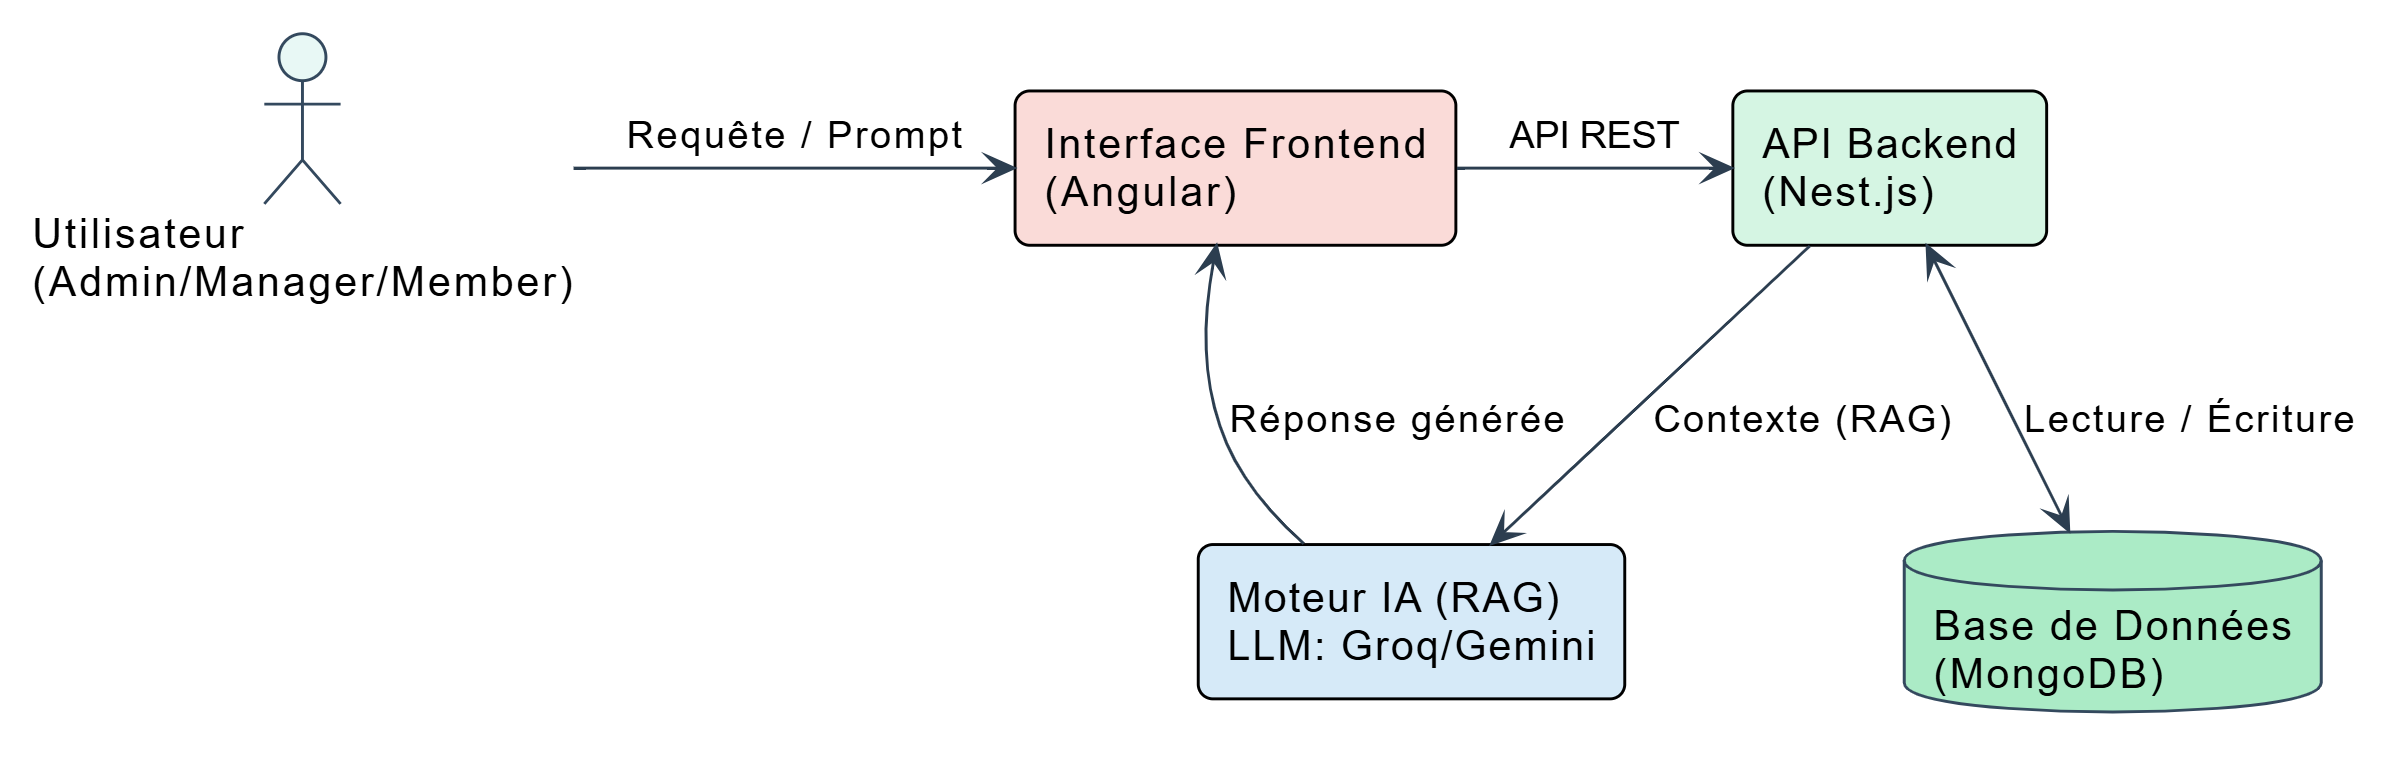
\includegraphics[width=0.9\textwidth]{images/flux_macroscopique.png}
  \caption{Diagramme de flux macroscopique de l'architecture intelligente SmartPM}
  \label{fig:flux_macroscopique}
\end{figure}
\vspace{0.3cm}


% ─────────────────────────────────────────────────────────
\section{Étude de faisabilité et gestion des risques}
\label{sec:faisabilite}
% ─────────────────────────────────────────────────────────

Avant d'entamer le développement, il est crucial d'évaluer la faisabilité du projet sous différents angles et 
d'anticiper les risques potentiels.

\subsection{Étude de faisabilité}

\begin{itemize}
  \item \textbf{Faisabilité technologique :} Le projet s'appuie sur des technologies open-source éprouvées (Node.js, Angular, MongoDB, Kubernetes). 
  L'intégration de l'IA est rendue possible grâce aux APIs modernes (Groq, Gemini) qui offrent des temps de réponse très rapides et une grande fiabilité. La mise en place de Kubernetes en environnement local (Minikube ou Docker Desktop) assure un développement fluide.
  
  \item \textbf{Faisabilité opérationnelle :} La solution web est accessible depuis n'importe quel navigateur, ne nécessitant aucune installation lourde pour les utilisateurs finaux (Managers, Développeurs). L'authentification OAuth2 (Google/GitHub) garantit une adoption rapide par les équipes informatiques.
\end{itemize}

\subsection{Analyse et gestion des risques}

Le tableau suivant répertorie les principaux risques identifiés et les mesures préventives adoptées :

\begin{table}[H]
  \centering
  \caption{Matrice d'analyse des risques}
  \label{tab:risques}
  \renewcommand{\arraystretch}{1.5}
  \begin{tabularx}{\textwidth}{|>{\hsize=.3\hsize}X|>{\hsize=.35\hsize}X|>{\hsize=.35\hsize}X|}
    \hline
    \rowcolor{tablehead}
    \textcolor{white}{\textbf{Type de Risque}} & \textcolor{white}{\textbf{Description}} & \textcolor{white}{\textbf{Mesures préventives / Solutions}} \\
    \hline
    \textbf{Risque Technologique} & Latence élevée lors des requêtes vers les modèles d'IA (LLMs) externes. & Implémentation d'un système de mise en cache et choix de Groq (connu pour sa très faible latence en inférence). \\
    \hline
    \textbf{Risque Infrastructure} & Complexité de configuration et de déploiement des clusters Kubernetes. & Création de scripts d'automatisation (fichiers YAML standardisés) et utilisation d'un environnement de test isolé. \\
    \hline
    \textbf{Risque Sécuritaire} & Fuite de données de projets sensibles via les APIs publiques. & Anonymisation des données critiques avant l'envoi aux LLMs et sécurisation des routes par des tokens JWT stricts. \\
    \hline
    \textbf{Risque Temporel} & Retard dans la livraison en raison de la courbe d'apprentissage sur de multiples outils (IA, K8s). & Adoption stricte de la méthodologie Scrum, permettant une réévaluation continue des priorités à chaque sprint. \\
    \hline
  \end{tabularx}
\end{table}


% ─────────────────────────────────────────────────────────
\section{Méthodologie et approche de gestion de projet}
\label{sec:methodologie}
% ─────────────────────────────────────────────────────────

La réussite d'un projet technologique complexe repose en grande partie sur l'adoption d'une méthodologie
de gestion adaptée. 

\subsection{Méthodes agiles et Scrum}

Dans le cadre du développement de SmartPM, nous avons opté pour la méthodologie \textbf{Scrum}, 
qui met l'accent sur la valeur métier du livrable, l'amélioration continue et la capacité à s'adapter aux changements 
via des itérations courtes appelées \textbf{Sprints}.

\vspace{0.3cm}

\textbf{Les rôles Scrum définis pour ce projet :}

\begin{itemize}
  \item \textbf{Product Owner :} Mohamed Anwer Tarhouni — Responsable de la vision produit, il définit les priorités du backlog et représente les besoins des utilisateurs finaux.
  \item \textbf{Scrum Master :} Mejda Bedoui — Facilitateur, elle veille à la bonne application des principes Scrum et aide à surmonter les obstacles techniques.
  \item \textbf{Équipe de développement :} Maher Raissi — En charge du développement Full-Stack, de l'intégration IA et de la mise en place de l'infrastructure DevOps.
\end{itemize}

\begin{figure}[H]
  \centering
  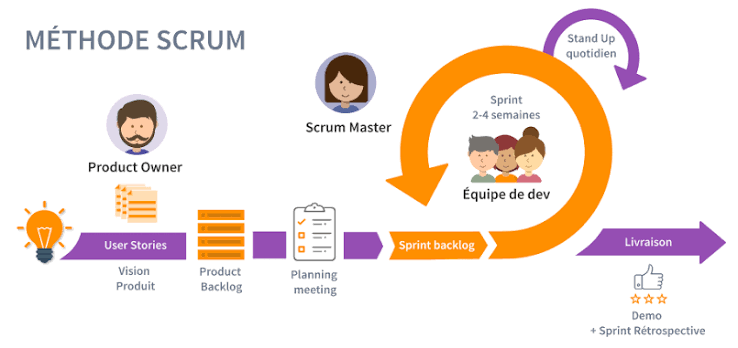
\includegraphics[width=0.9\textwidth]{images/scrum_cycle.png}
  \caption{Cycle de vie de la m\'ethodologie Scrum}
  \label{fig:scrum_cycle}
\end{figure}

\subsection{Planification et Chronogramme (Sprints)}

Le cycle de développement a été découpé en plusieurs sprints stratégiques afin de garantir des livraisons progressives et fonctionnelles :

\begin{itemize}
  \item \textbf{Sprint 0 : Initiation et conception.} Définition de l'architecture logicielle, analyse des besoins, élaboration des diagrammes UML et choix des technologies (Angular, Node.js).
  \item \textbf{Sprint 1 : Socle fonctionnel et Backend.} Mise en place de l'authentification (JWT, OAuth2), conception de la base de données MongoDB, et développement des opérations CRUD pour les projets et les tâches.
  \item \textbf{Sprint 2 : Frontend et Expérience utilisateur.} Développement des interfaces avec Angular (Dashboards, vues Kanban, gestion des utilisateurs) et liaison avec l'API Backend.
  \item \textbf{Sprint 3 : Intelligence Artificielle.} Intégration des modèles LLM, développement du chatbot contextuel et implémentation de la génération automatique des rapports.
  \item \textbf{Sprint 4 : Déploiement DevOps et Observabilité.} Containerisation avec Docker, écriture des manifestes Kubernetes, configuration du monitoring (Prometheus \& Grafana) et tests finaux.
\end{itemize}

\subsection{Méthodologie de conception (UML)}

Pour la conception logicielle de SmartPM, nous avons adopté le langage \textbf{UML} (Unified Modeling Language). 
Les diagrammes qui guideront notre conception dans les chapitres suivants sont :

\begin{itemize}
  \item \textbf{Diagramme de cas d'utilisation :} Modélise les interactions entre les utilisateurs (Admin, Manager, Member) et le système.
  \item \textbf{Diagramme de classes :} Représente l'architecture statique de la base de données et des entités métiers.
  \item \textbf{Diagramme de séquence :} Détaille les flux d'informations temporels (ex: processus d'authentification ou interaction avec l'IA).
  \item \textbf{Diagramme d'activités :} Illustre la logique des processus complexes (ex: le pipeline de génération de rapport par l'IA).
\end{itemize}

% ─────────────────────────────────────────────────────────
\section*{Conclusion}
% ─────────────────────────────────────────────────────────

Ce chapitre a permis de situer SmartPM dans son contexte général en présentant l'organisme
d'accueil Capgemini Tunisie, tout en mettant en évidence l'évolution du marché vers une gestion 
de projet plus intelligente et automatisée. L'étude critique de l'existant a confirmé la nécessité 
d'une solution innovante alliant l'Intelligence Artificielle générative et une architecture Cloud-Native robuste.
L'analyse de faisabilité et la gestion des risques nous ont permis de valider la viabilité technique du projet. 
Enfin, nous avons défini le cadre méthodologique Scrum et planifié les sprints qui structureront la réalisation.

\vspace{0.3cm}

Le chapitre suivant sera consacré à l'analyse approfondie des besoins fonctionnels et non-fonctionnels, 
ainsi qu'à la conception architecturale détaillée du système SmartPM via les diagrammes UML.

% ============================================================
%  CHAPITRE 2 — ANALYSE ET SPÉCIFICATION DES BESOINS
% ============================================================
\chapter{Analyse et spécification des besoins}

\vspace{-0.5cm}
\begin{tcolorbox}[colback=lightgray, colframe=primaryblue, title=\textbf{Plan du chapitre}, fonttitle=\bfseries]
  \begin{enumerate}[leftmargin=*, label=\arabic*.]
    \item Spécification des besoins \dotfill \pageref{sec:besoins}
    \item Analyse globale \dotfill \pageref{sec:analyse_globale}
    \item Élaboration du Backlog produit \dotfill \pageref{sec:backlog}
    \item Planification du travail \dotfill \pageref{sec:planification}
    \item Architecture de la solution \dotfill \pageref{sec:architecture}
    \item Choix techniques \dotfill \pageref{sec:choix_techniques}
    \item Mise en place de la solution DevOps \dotfill \pageref{sec:devops}
  \end{enumerate}
\end{tcolorbox}

% ─────────────────────────────────────────────────────────
\section*{Introduction}
% ─────────────────────────────────────────────────────────

Ce chapitre a pour objectif de présenter l'ensemble des acteurs impliqués dans la plateforme
SmartPM ainsi que les besoins fonctionnels et non fonctionnels qui lui sont associés. Cette
première étape permettra de structurer le backlog produit et de garantir une compréhension
précise et partagée des exigences du projet.

Dans un second temps, une analyse globale sera réalisée à travers des diagrammes UML~\cite{uml} afin
de décrire l'architecture à adopter pour la solution proposée. Enfin, le chapitre se conclura
par la planification des sprints, illustrant l'organisation et le déroulement du développement.


% ─────────────────────────────────────────────────────────
\section{Spécification des besoins}
\label{sec:besoins}
% ─────────────────────────────────────────────────────────

\subsection{Identification des acteurs}

Afin de bien comprendre le périmètre et les interactions de la plateforme SmartPM, nous
identifions dans cette section les différents acteurs qui interagissent avec le système.
SmartPM comporte trois rôles d'utilisateurs internes principaux :

\subsubsection{Administrateur (Admin)}

L'administrateur est le super-utilisateur de la plateforme. Il dispose d'un accès complet
à l'ensemble des fonctionnalités de configuration et de supervision. Son rôle principal est
de gérer les comptes utilisateurs, d'assigner les rôles, de consulter les journaux d'audit
et de maintenir la cohérence des données du système.

\subsubsection{Manager (Chef de projet)}

Le Manager est l'utilisateur central de SmartPM. Il est responsable de la création et de
la supervision des projets qui lui sont confiés. Il dispose d'un tableau de bord dédié lui
offrant une vision globale de l'avancement de ses projets, de la charge de son équipe et des
métriques clés. Il peut créer des projets via un wizard multi-étapes, affecter des membres
à des tâches et générer des rapports grâce à l'intelligence artificielle intégrée.

\subsubsection{Member (Membre d'équipe)}

Le Member est un collaborateur affecté à un ou plusieurs projets. Il dispose d'un tableau
de bord personnel lui présentant ses tâches en cours, ses certifications à valider et ses
revues en attente. Il peut soumettre des revues de tâches (dans le respect de la règle
Author~$\neq$~Reviewer) et utiliser l'assistant IA pour obtenir de l'aide sur ses tâches.

\vspace{0.3cm}

\begin{figure}[H]
  \centering
  \begin{tikzpicture}[
      scale=1.1, transform shape,
      actor/.style={draw, rounded corners=8pt, thick, align=center, minimum width=3.8cm, minimum height=2cm},
      admin/.style={actor, draw=red!70, fill=red!5, text=red!80!black},
      manager/.style={actor, draw=primaryblue!80, fill=primaryblue!5, text=primaryblue!80!black},
      member/.style={actor, draw=successgreen!80, fill=successgreen!5, text=successgreen!80!black},
      platform/.style={draw=darkgray, very thick, rounded corners=12pt, fill=gray!5, minimum width=4cm, minimum height=2.5cm, align=center, font=\Large\bfseries\color{primaryblue}}
  ]
      % Acteurs
      \node[admin] (admin) at (-5, 3) {\LARGE\faUserShield\\[0.1cm]\normalsize\textbf{Administrateur}\\[0.1cm]\scriptsize Supervision globale};
      \node[manager] (manager) at (-5, 0) {\LARGE\faUserTie\\[0.1cm]\normalsize\textbf{Manager}\\[0.1cm]\scriptsize Gestion des projets};
      \node[member] (member) at (-5, -3) {\LARGE\faUser\\[0.1cm]\normalsize\textbf{Member}\\[0.1cm]\scriptsize R\'ealisation des t\^aches};

      % Plateforme
      \node[platform] (sys) at (0, 0) {\faRocket\\[0.1cm] SmartPM};

      % Lignes
      \draw[very thick, -stealth, darkgray] (admin) -| (sys.north);
      \draw[very thick, -stealth, darkgray] (manager) -- (sys);
      \draw[very thick, -stealth, darkgray] (member) -| (sys.south);
  \end{tikzpicture}
  \caption{Sch\'ema des acteurs de la plateforme SmartPM}
  \label{fig:acteurs}
\end{figure}

\subsection{Identification des besoins fonctionnels}

La plateforme SmartPM doit répondre aux besoins fonctionnels suivants, répartis par acteur :

\vspace{0.3cm}
\textbf{L'Administrateur doit pouvoir :}
\begin{itemize}
  \item Créer, modifier, désactiver et supprimer des comptes utilisateurs
  \item Assigner et modifier les rôles des utilisateurs (Admin / Manager / Member)
  \item Consulter les journaux d'audit (actions, connexions, modifications)
  \item Réinitialiser les mots de passe des utilisateurs
  \item Superviser les métriques globales de la plateforme (Prometheus/Grafana)
\end{itemize}

\vspace{0.3cm}
\textbf{Le Manager doit pouvoir :}
\begin{itemize}
  \item Créer un projet via un wizard multi-étapes (nom, description, dates, équipe)
  \item Gérer la hiérarchie des tâches : Activités~$\rightarrow$ Sous-Activités~$\rightarrow$ Tâches
  \item Affecter des tâches à des membres et définir leurs échéances et priorités
  \item Suivre l'avancement global du projet via un tableau de bord dédié
  \item Utiliser l'IA pour simuler l'avancement du projet et générer des rapports
  \item Consulter les certifications et revues de son équipe
\end{itemize}

\vspace{0.3cm}
\textbf{Le Member doit pouvoir :}
\begin{itemize}
  \item Consulter ses tâches assignées et leur statut
  \item Mettre à jour le statut de ses tâches (TODO / IN\_PROGRESS / IN\_REVIEW / DONE)
  \item Soumettre des revues sur des tâches (Author~$\neq$~Reviewer)
  \item Valider les certifications correspondant à sa phase courante (HLR/LLR/CODE/LLT/HLT)
  \item Commenter des tâches et recevoir des notifications en temps réel
  \item Interagir avec le chatbot IA pour obtenir des réponses contextuelles
\end{itemize}

\subsection{Identification des besoins non fonctionnels}

L'efficacité de SmartPM repose non seulement sur ses fonctionnalités, mais également sur
des aspects non fonctionnels garantissant une expérience utilisateur optimale et la fiabilité
du système.

\begin{itemize}
  \item \textbf{Sécurité :} Authentification JWT avec expiration configurable, OAuth2 via Google
  et GitHub, protection CORS stricte, en-têtes de sécurité HTTP via Helmet, rate limiting
  (100 requêtes/minute par IP) contre les attaques DDoS et brute-force.

  \item \textbf{Performance :} Temps de réponse API inférieur à 2 secondes pour les opérations
  courantes, réponse du chatbot IA en moins d'une seconde grâce à Groq (streaming SSE).

  \item \textbf{Disponibilité :} Architecture Kubernetes avec 2 réplicas pour le backend et
  le frontend, garantissant une haute disponibilité et une tolérance aux pannes.

  \item \textbf{Scalabilité :} Architecture modulaire NestJS permettant l'ajout de nouveaux
  modules sans impact sur les fonctionnalités existantes. Kubernetes permet le scaling horizontal
  automatique selon la charge.

  \item \textbf{Maintenabilité :} Code TypeScript strict, architecture en couches (Controller /
  Service / Repository), documentation API auto-générée via Swagger.

  \item \textbf{Observabilité :} Monitoring en temps réel via Prometheus (métriques API,
  latence, erreurs) et Grafana (dashboards visuels). Backup automatique de la base de données
  MongoDB Atlas.
\end{itemize}


% ─────────────────────────────────────────────────────────
\section{Analyse globale}
\label{sec:analyse_globale}
% ─────────────────────────────────────────────────────────

\subsection{Diagramme de cas d'utilisation global}

La figure~\ref{fig:use_case_global} présente le diagramme de cas d'utilisation global de la
plateforme SmartPM, illustrant les interactions entre les trois acteurs principaux et les
fonctionnalités du système.

\begin{figure}[H]
  \centering
  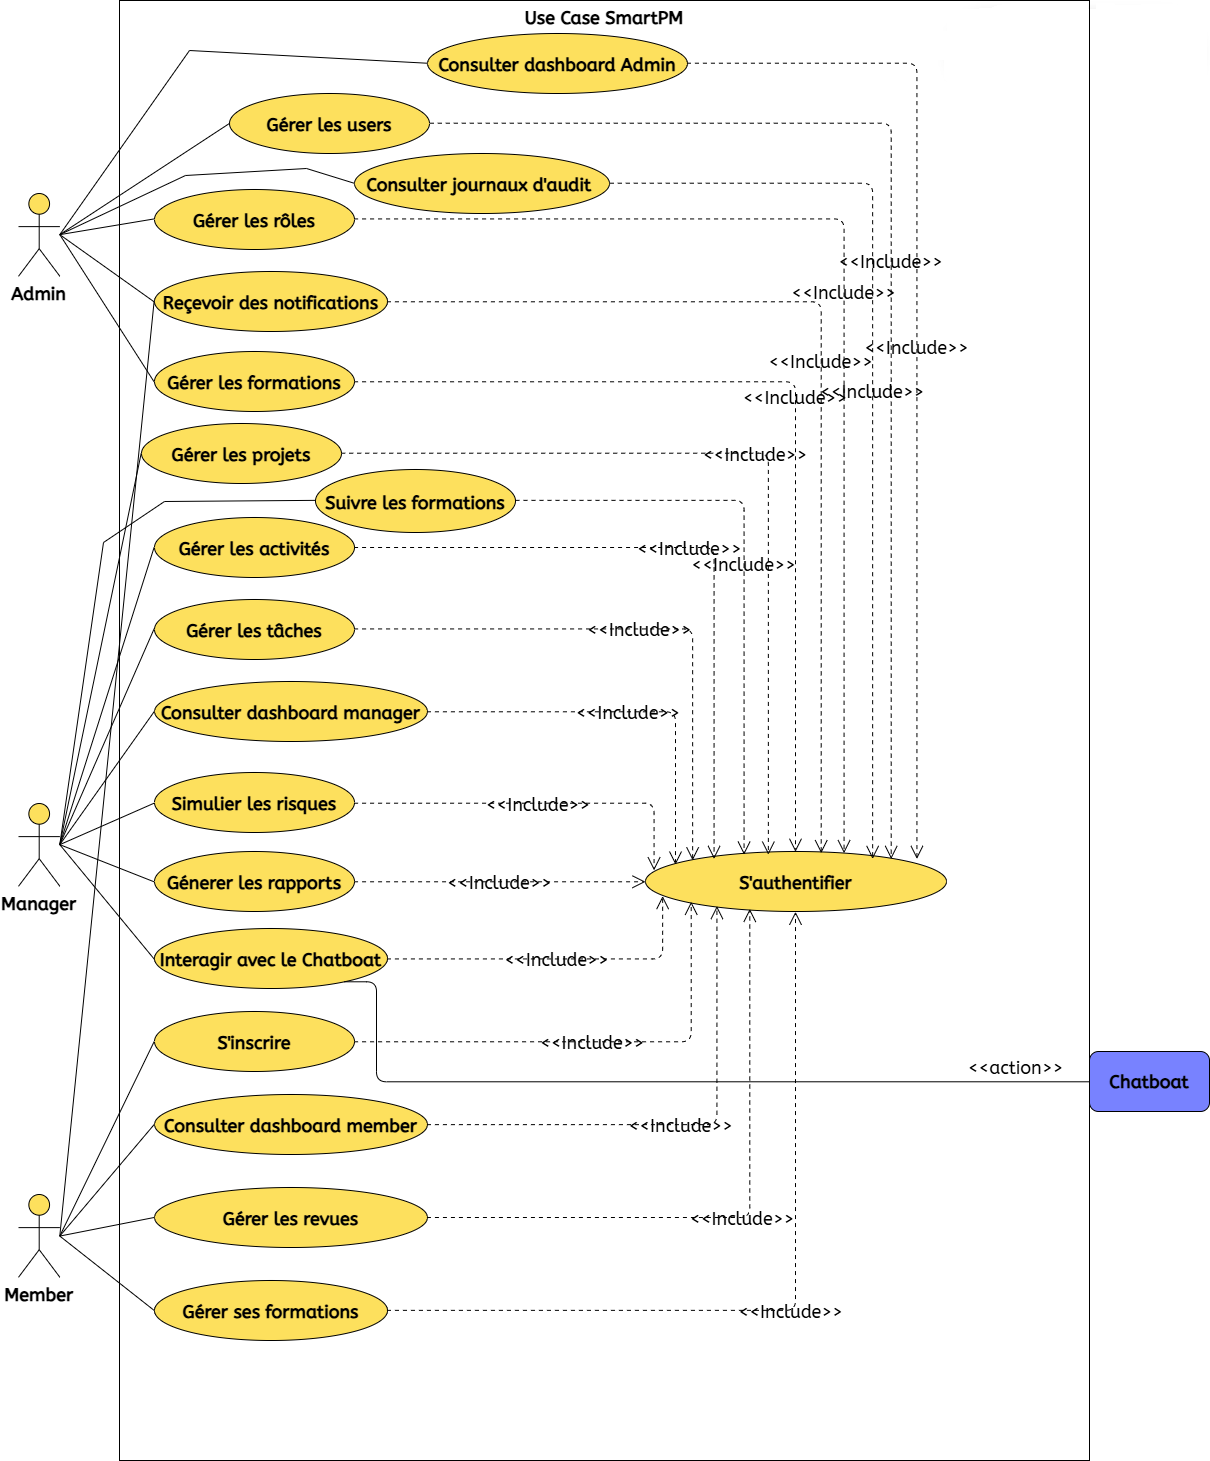
\includegraphics[width=\textwidth]{images/diagram-usecase.png}
  \caption{Diagramme de cas d'utilisation global de SmartPM}
  \label{fig:use_case_global}
\end{figure}

\subsection{Diagramme de classes global}

La figure~\ref{fig:class_global} présente le diagramme de classes global de SmartPM,
illustrant la structure des principales entités du système et leurs relations.

\begin{figure}[H]
  \centering
  \includegraphics[width=\textwidth]{images/diagram-classes.jpg}
  \caption{Diagramme de classes global de SmartPM}
  \label{fig:class_global}
\end{figure}


% ─────────────────────────────────────────────────────────
\section{Élaboration du Backlog produit}
\label{sec:backlog}
% ─────────────────────────────────────────────────────────

Dans Scrum, le Backlog produit regroupe l'ensemble des exigences liées au produit,
transformées en User Stories. Chaque User Story décrit une fonctionnalité du point de vue
de l'utilisateur et est associée à une priorité et une charge estimée.

Notre tableau~\ref{tab:backlog} est caractérisé par les champs suivants :
\begin{itemize}
  \item \textbf{ID} : Identifiant unique auto-incrémenté
  \item \textbf{User Story} : Scénario décrivant la valeur ajoutée de la fonctionnalité
  \item \textbf{Priorité} : Valeur numérique (1 = haute, 4 = basse)
  \item \textbf{Charge} : Estimation en jours de développement
\end{itemize}

\begin{longtable}{|c|p{7cm}|c|c|}
  \caption{Backlog produit global de SmartPM}
  \label{tab:backlog} \\
  \hline
  \rowcolor{tablehead}
  \textcolor{white}{\textbf{ID}} &
  \textcolor{white}{\textbf{User Story}} &
  \textcolor{white}{\textbf{Priorité}} &
  \textcolor{white}{\textbf{Charge (j)}} \\
  \hline
  \endfirsthead
  \multicolumn{4}{c}{\textit{Suite du Backlog produit}} \\
  \hline
  \textbf{ID} & \textbf{User Story} & \textbf{Priorité} & \textbf{Charge} \\
  \hline
  \endhead
  \hline
  \endfoot

  % Sprint 1
  \multicolumn{4}{|c|}{\cellcolor{primaryblue!20}\textbf{Sprint 1 — Authentification \& Gestion des utilisateurs}} \\
  \hline
  US01 & En tant qu'utilisateur, je peux m'authentifier avec email/mot de passe via JWT & 1 & 4 \\
  \hline
  US02 & En tant qu'utilisateur, je peux me connecter via Google OAuth2 & 2 & 3 \\
  \hline
  US03 & En tant qu'utilisateur, je peux me connecter via GitHub OAuth2 & 2 & 2 \\
  \hline
  US04 & En tant qu'Admin, je peux créer, modifier et désactiver des comptes utilisateurs & 1 & 3 \\
  \hline
  US05 & En tant qu'Admin, je peux assigner/modifier les rôles des utilisateurs & 1 & 2 \\
  \hline
  US06 & En tant qu'Admin, je consulte les journaux d'audit (connexions, actions) & 3 & 2 \\
  \hline

  % Sprint 2
  \multicolumn{4}{|c|}{\cellcolor{primaryblue!20}\textbf{Sprint 2 — Gestion des projets, activités et tâches}} \\
  \hline
  US07 & En tant que Manager, je crée un projet via un wizard multi-étapes & 1 & 5 \\
  \hline
  US08 & En tant que Manager, je gère les activités d'un projet (CRUD) & 1 & 3 \\
  \hline
  US09 & En tant que Manager, je gère les sous-activités (CRUD) & 2 & 3 \\
  \hline
  US10 & En tant que Manager, je crée et assigne des tâches aux membres & 1 & 4 \\
  \hline
  US11 & En tant que Manager, je consulte le tableau de bord global de mes projets & 2 & 3 \\
  \hline
  US12 & En tant que Member, je consulte mon tableau de bord personnel (tâches, certif.) & 2 & 3 \\
  \hline

  % Sprint 3
  \multicolumn{4}{|c|}{\cellcolor{primaryblue!20}\textbf{Sprint 3 — Revues, certifications \& notifications}} \\
  \hline
  US13 & En tant que Member, je soumets une revue sur une tâche (Author $\neq$ Reviewer) & 1 & 4 \\
  \hline
  US14 & En tant que Member, je valide ou rejette une revue soumise par un pair & 1 & 3 \\
  \hline
  US15 & En tant que Member, je valide une certification pour une phase DO-178C & 2 & 4 \\
  \hline
  US16 & En tant qu'utilisateur, je commente une tâche (fil de discussion) & 3 & 2 \\
  \hline
  US17 & En tant qu'utilisateur, je reçois des notifications en temps réel & 3 & 3 \\
  \hline

  % Sprint 4
  \multicolumn{4}{|c|}{\cellcolor{primaryblue!20}\textbf{Sprint 4 — Intelligence artificielle \& Formations}} \\
  \hline
  US18 & En tant qu'utilisateur, j'interagis avec le chatbot AI contextuel (données live) & 1 & 5 \\
  \hline
  US19 & En tant que Manager, je simule l'avancement et les risques de mon projet via l'IA & 2 & 4 \\
  \hline
  US20 & En tant que Manager, je génère un rapport de projet automatique via l'IA & 3 & 3 \\
  \hline
  US21 & En tant qu'utilisateur, j'accède aux formations (PDF/vidéo) liées au projet & 4 & 3 \\
  \hline

  % Sprint 5
  \multicolumn{4}{|c|}{\cellcolor{primaryblue!20}\textbf{Sprint 5 — DevOps, monitoring \& sécurité}} \\
  \hline
  US22 & Le système est containerisé via Docker (3 images : frontend, backend, AI) & 1 & 3 \\
  \hline
  US23 & Le système est déployé sur Kubernetes avec haute disponibilité (6 pods) & 1 & 5 \\
  \hline
  US24 & Les métriques sont collectées par Prometheus et visualisées dans Grafana & 2 & 4 \\
  \hline
  US25 & Le système implémente Helmet, CORS strict et Rate Limiting (100 req/min) & 1 & 2 \\
  \hline
  US26 & Le backup automatique MongoDB est configuré et testé & 3 & 2 \\
  \hline
\end{longtable}


% ─────────────────────────────────────────────────────────
\section{Planification du travail}
\label{sec:planification}
% ─────────────────────────────────────────────────────────

\subsection{Répartition des sprints par release}

Le tableau~\ref{tab:sprints} présente la répartition des sprints par release, avec leur
durée et leur objectif principal.

\begin{table}[H]
  \centering
  \caption{Planification des sprints par release}
  \label{tab:sprints}
  \renewcommand{\arraystretch}{1.5}
  \begin{tabularx}{\textwidth}{|c|c|X|c|}
    \hline
    \rowcolor{tablehead}
    \textcolor{white}{\textbf{Release}} &
    \textcolor{white}{\textbf{Sprint}} &
    \textcolor{white}{\textbf{Titre}} &
    \textcolor{white}{\textbf{Durée}} \\
    \hline
    \multirow{3}{*}{\textbf{Release 1}} &
    Sprint 1 & Authentification \& Gestion des utilisateurs & 2 semaines \\
    \cline{2-4}
    & Sprint 2 & Gestion des projets, activités et tâches & 2 semaines \\
    \cline{2-4}
    & Sprint 3 & Revues, certifications \& notifications & 2 semaines \\
    \hline
    \multirow{2}{*}{\textbf{Release 2}} &
    Sprint 4 & Intelligence artificielle \& Formations & 2 semaines \\
    \cline{2-4}
    & Sprint 5 & DevOps, monitoring \& sécurité & 2 semaines \\
    \hline
    \multicolumn{2}{|c|}{\textbf{Total}} &
    \textbf{5 sprints — 2 releases} & \textbf{10 semaines} \\
    \hline
  \end{tabularx}
\end{table}

\subsection{Planification globale des sprints}

La figure~\ref{fig:gantt} illustre la planification globale des sprints sous forme de
diagramme de Gantt, permettant de visualiser l'enchaînement temporel des différentes
phases du projet.

\begin{figure}[H]
  \centering
  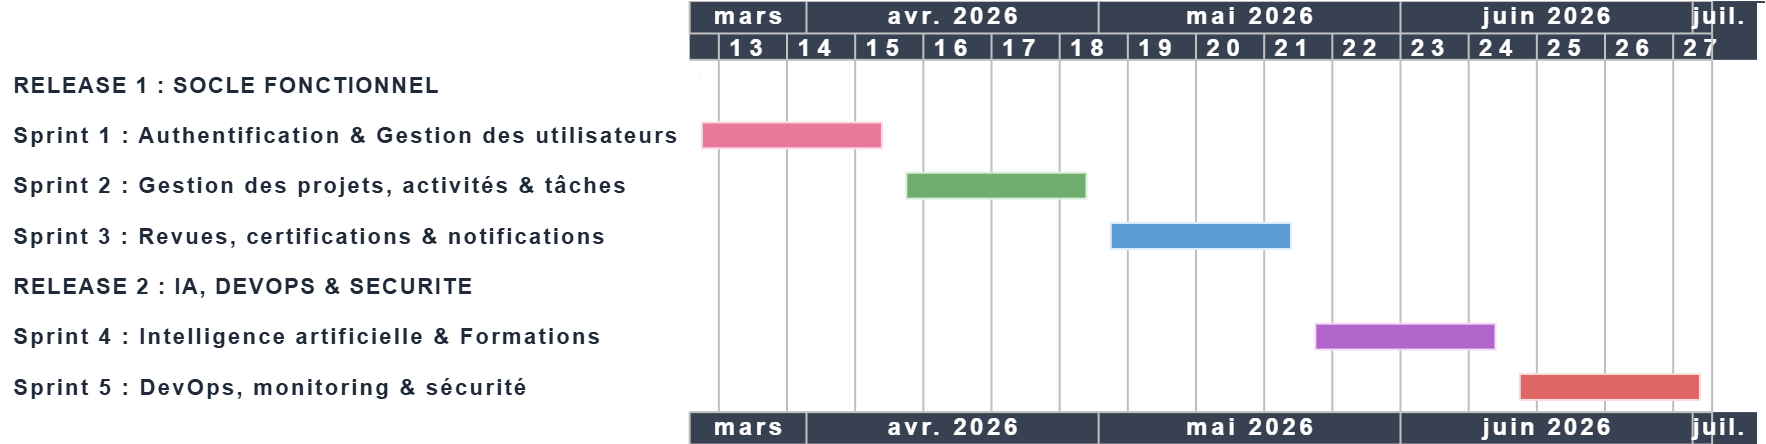
\includegraphics[width=\textwidth]{images/gantt.png}
  \caption{Planification globale des sprints (diagramme de Gantt)}
  \label{fig:gantt}
\end{figure}


% ─────────────────────────────────────────────────────────
\section{Architecture de la solution}
\label{sec:architecture}
% ─────────────────────────────────────────────────────────

\subsection{Architecture physique}

L'architecture physique de SmartPM repose sur un modèle \textbf{3-tiers}~\cite{arch3tiers} classique,
séparant la couche présentation, la couche métier et la couche données.

\begin{itemize}
  \item \textbf{Couche présentation :} Application Angular~19 (Single Page Application),
  servie par un conteneur Nginx exposé via le NodePort 30080 de Kubernetes.

  \item \textbf{Couche métier :} API REST développée avec NestJS, exposée via le
  NodePort~30000. Elle gère l'ensemble de la logique métier, l'authentification JWT,
  et la coordination avec les autres services.

  \item \textbf{Service IA :} Microservice FastAPI (Python) exposé via le NodePort~30800,
  responsable du chatbot contextuel et des simulations de projets.

  \item \textbf{Couche données :} MongoDB Atlas, base de données NoSQL hébergée en
  cloud, accessible depuis le cluster Kubernetes via une connexion sécurisée TLS.
\end{itemize}

\begin{figure}[H]
  \centering
  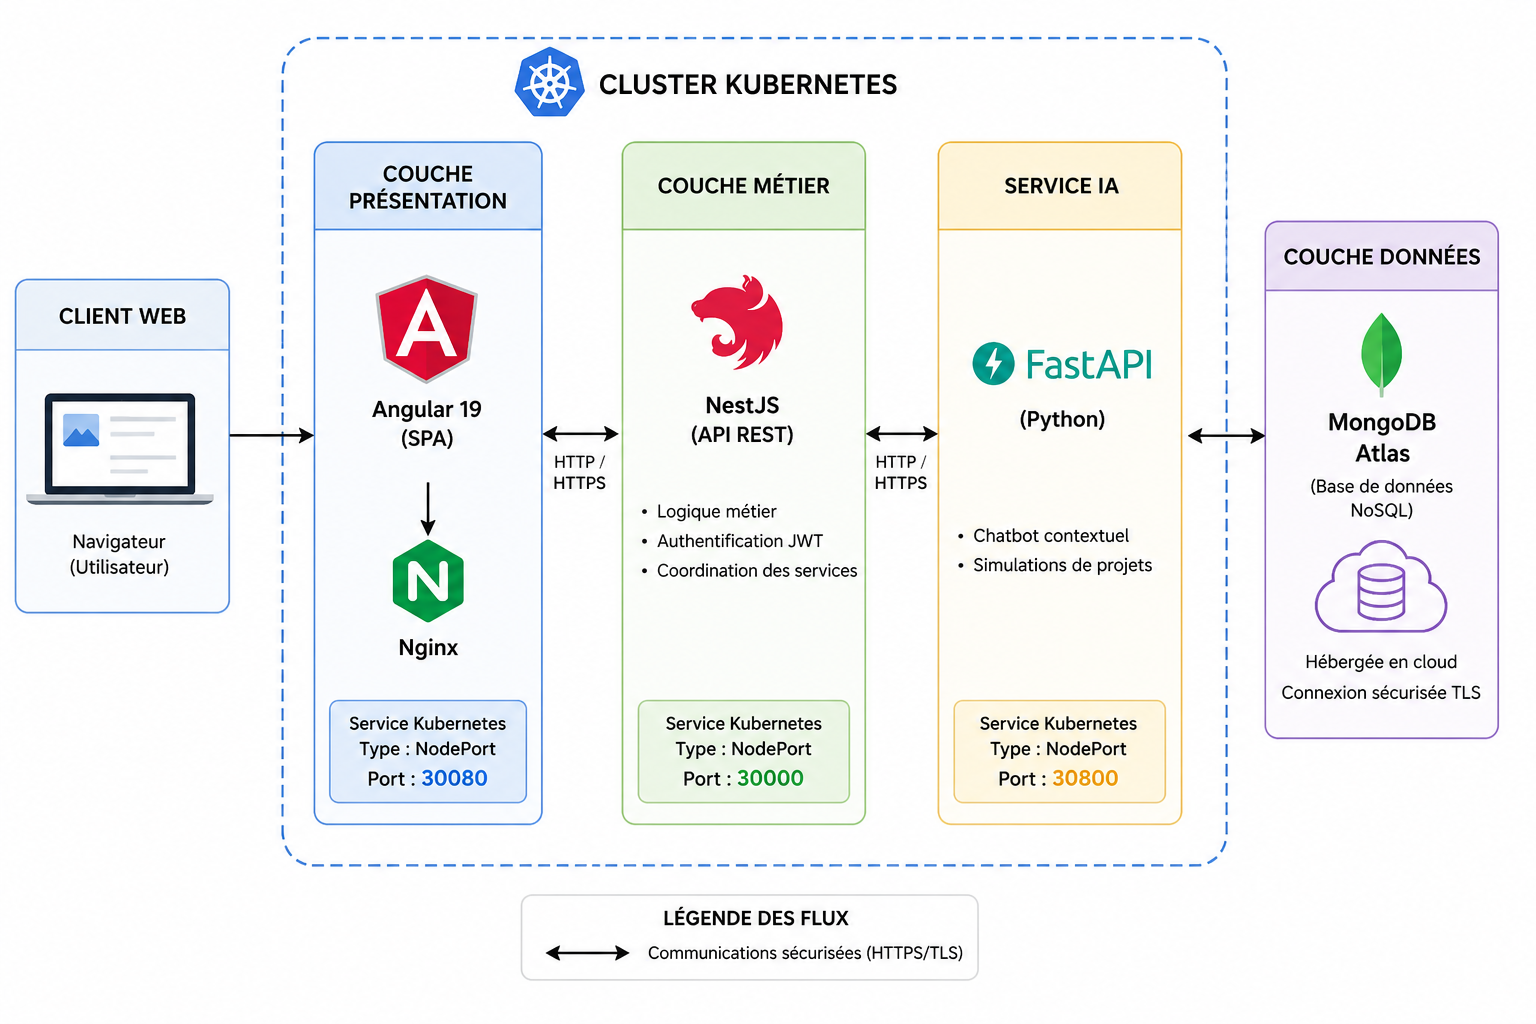
\includegraphics[width=0.9\textwidth]{images/architecture_physique.png}
  \caption{Architecture physique 3-tiers de SmartPM}
  \label{fig:archi_physique}
\end{figure}

\subsection{Architecture logicielle}

L'architecture logicielle de SmartPM suit le patron \textbf{MVC}~\cite{mvc} (Model-View-Controller)
côté backend, complété par une architecture modulaire propre à NestJS~\cite{nestjs}.

\begin{itemize}
  \item \textbf{Frontend (Angular 19)~\cite{angular} :} Architecture par composants avec services injectables
  pour la communication avec l'API. Chaque fonctionnalité est encapsulée dans un module Angular
  autonome (AuthModule, ProjectModule, AiChatbotModule...).

  \item \textbf{Backend (NestJS) :} Architecture modulaire avec séparation claire des
  responsabilités (Controller~$\rightarrow$ Service~$\rightarrow$ Schema Mongoose). Les modules
  indépendants sont : AuthModule, UserModule, ProjectModule, ActivityModule, SubActivityModule,
  TaskModule, ReviewModule, CertificationModule, NotificationModule, CommentModule,
  AiIntegrationModule, TrainingModule, AdminModule.

  \item \textbf{Service IA (FastAPI) :} Architecture orientée routes avec gestion asynchrone
  des requêtes et streaming SSE (Server-Sent Events) pour les réponses en temps réel.
\end{itemize}

\begin{figure}[H]
  \centering
  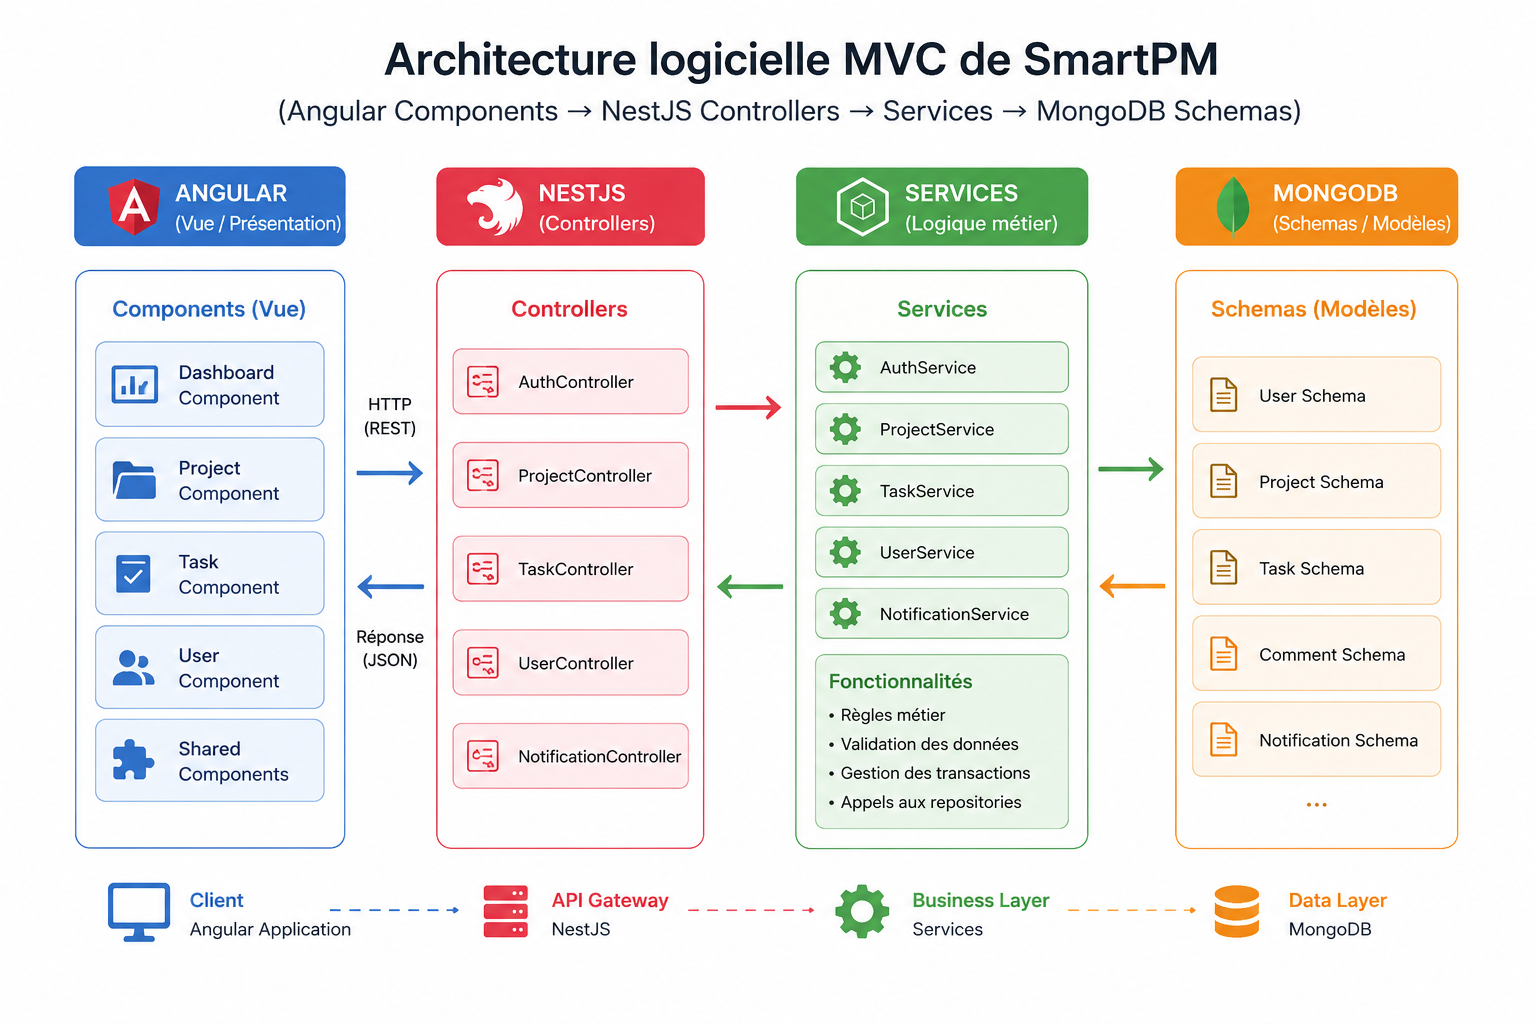
\includegraphics[width=0.85\textwidth]{images/architecture_logicielle.png}
  \caption{Architecture logicielle de SmartPM}
  \label{fig:archi_logicielle}
\end{figure}

\subsection{Architecture IA multi-modèles}

Le service IA de SmartPM est conçu selon une architecture \textbf{multi-LLM avec fallback},
garantissant la disponibilité du chatbot même en cas de saturation d'un fournisseur.

\begin{enumerate}
  \item \textbf{Groq (Llama 3.1-8b-instant)}~\cite{groq} — fournisseur principal, temps de réponse
  très court (approx 300ms Time-To-First-Token).
  \item \textbf{Gemini 2.5 Flash (Google)}~\cite{gemini} — premier fallback, haute qualité de réponse.
  \item \textbf{OpenRouter (Mistral 7B)}~\cite{openrouter} — second fallback, solution open-source.
\end{enumerate}

\begin{figure}[H]
  \centering
  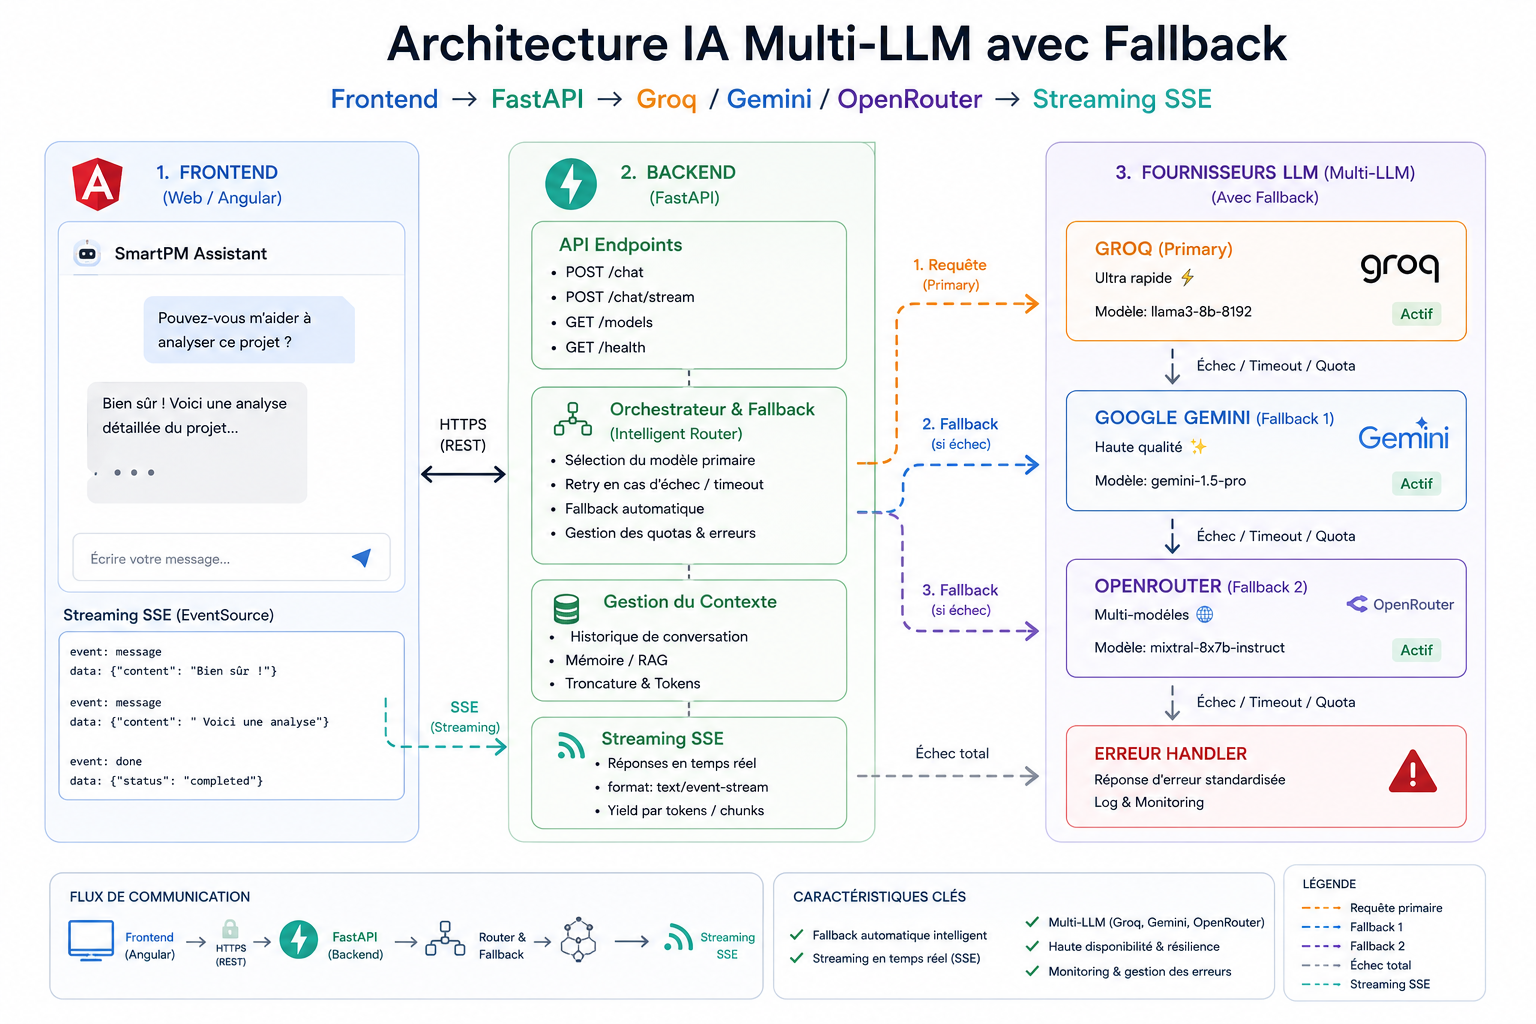
\includegraphics[width=0.8\textwidth]{images/architecture_ai.png}
  \caption{Architecture du système IA multi-modèles de SmartPM}
  \label{fig:archi_ai}
\end{figure}


% ─────────────────────────────────────────────────────────
\section{Choix techniques}
\label{sec:choix_techniques}
% ─────────────────────────────────────────────────────────

Le tableau~\ref{tab:choix_tech} récapitule les technologies retenues pour le développement
de SmartPM, accompagnées des justifications de chaque choix.

\begin{table}[H]
  \centering
  \caption{Tableau des choix techniques de SmartPM}
  \label{tab:choix_tech}
  \renewcommand{\arraystretch}{1.5}
  \begin{tabularx}{\textwidth}{|l|l|l|X|}
    \hline
    \rowcolor{tablehead}
    \textcolor{white}{\textbf{Couche}} &
    \textcolor{white}{\textbf{Technologie}} &
    \textcolor{white}{\textbf{Version}} &
    \textcolor{white}{\textbf{Justification}} \\
    \hline
    Frontend & Angular & 19 & SPA moderne, TypeScript strict, écosystème mature \\
    \hline
    Backend & NestJS & 11 & Architecture modulaire, decorators, JWT intégré, production-ready \\
    \hline
    Service IA & FastAPI & Python 3.11 & Asynchrone, SSE natif, excellent support LLM \\
    \hline
    Base de données & MongoDB Atlas & 7.0 & Flexibilité NoSQL, cloud natif, scalabilité horizontale \\
    \hline
    LLM Principal & Groq / Llama 3.1 & API & Rapidité $\approx$300ms TTFT, open-source, gratuit \\
    \hline
    LLM Fallback 1 & Gemini 2.5 Flash & API & Haute qualité, contexte large (1M tokens) \\
    \hline
    LLM Fallback 2 & OpenRouter / Mistral & API & Redondance, solution open-source \\
    \hline
    Conteneurisation & Docker & 26 & Portabilité, isolation, déploiement reproductible \\
    \hline
    Orchestration & Kubernetes & 1.30 & Scalabilité, haute disponibilité, rolling updates \\
    \hline
    Monitoring & Prometheus + Grafana & — & Métriques temps réel, dashboards visuels \\
    \hline
    Authentification & JWT + OAuth2 & — & Standard industrie, sécurité, stateless \\
    \hline
    Sécurité HTTP & Helmet + Throttler & — & Protection XSS, clickjacking, DDoS, brute-force \\
    \hline
    Proxy & Nginx & 1.25 & Serveur de fichiers statiques, performances élevées \\
    \hline
    Serveur Node & Node.js & 22 LTS & Runtime performant, non-bloquant, écosystème npm \\
    \hline
  \end{tabularx}
\end{table}


% ─────────────────────────────────────────────────────────
\section{Mise en place de la solution DevOps}
\label{sec:devops}
% ─────────────────────────────────────────────────────────

\subsection{Pipeline DevOps}

La solution DevOps de SmartPM repose sur un pipeline automatisé permettant de passer
du code source à un déploiement en production de manière reproductible et fiable.
Le pipeline se déroule en quatre étapes principales :

\begin{enumerate}
  \item \textbf{Build :} Construction des images Docker pour les trois services (Angular/Nginx,
  NestJS, FastAPI) à partir de Dockerfiles optimisés multi-stage.

  \item \textbf{Load :} Chargement des images dans le registre local de Minikube via la
  commande \texttt{minikube image load}, évitant la dépendance à un registre distant.

  \item \textbf{Deploy :} Application des manifestes Kubernetes (fichiers YAML) définissant
  les Deployments, Services, ConfigMaps et Secrets pour chacun des 6 pods.

  \item \textbf{Monitor :} Collecte automatique des métriques par Prometheus et visualisation
  dans Grafana, avec alertes configurables sur les seuils de performance.
\end{enumerate}

\begin{figure}[H]
  \centering
  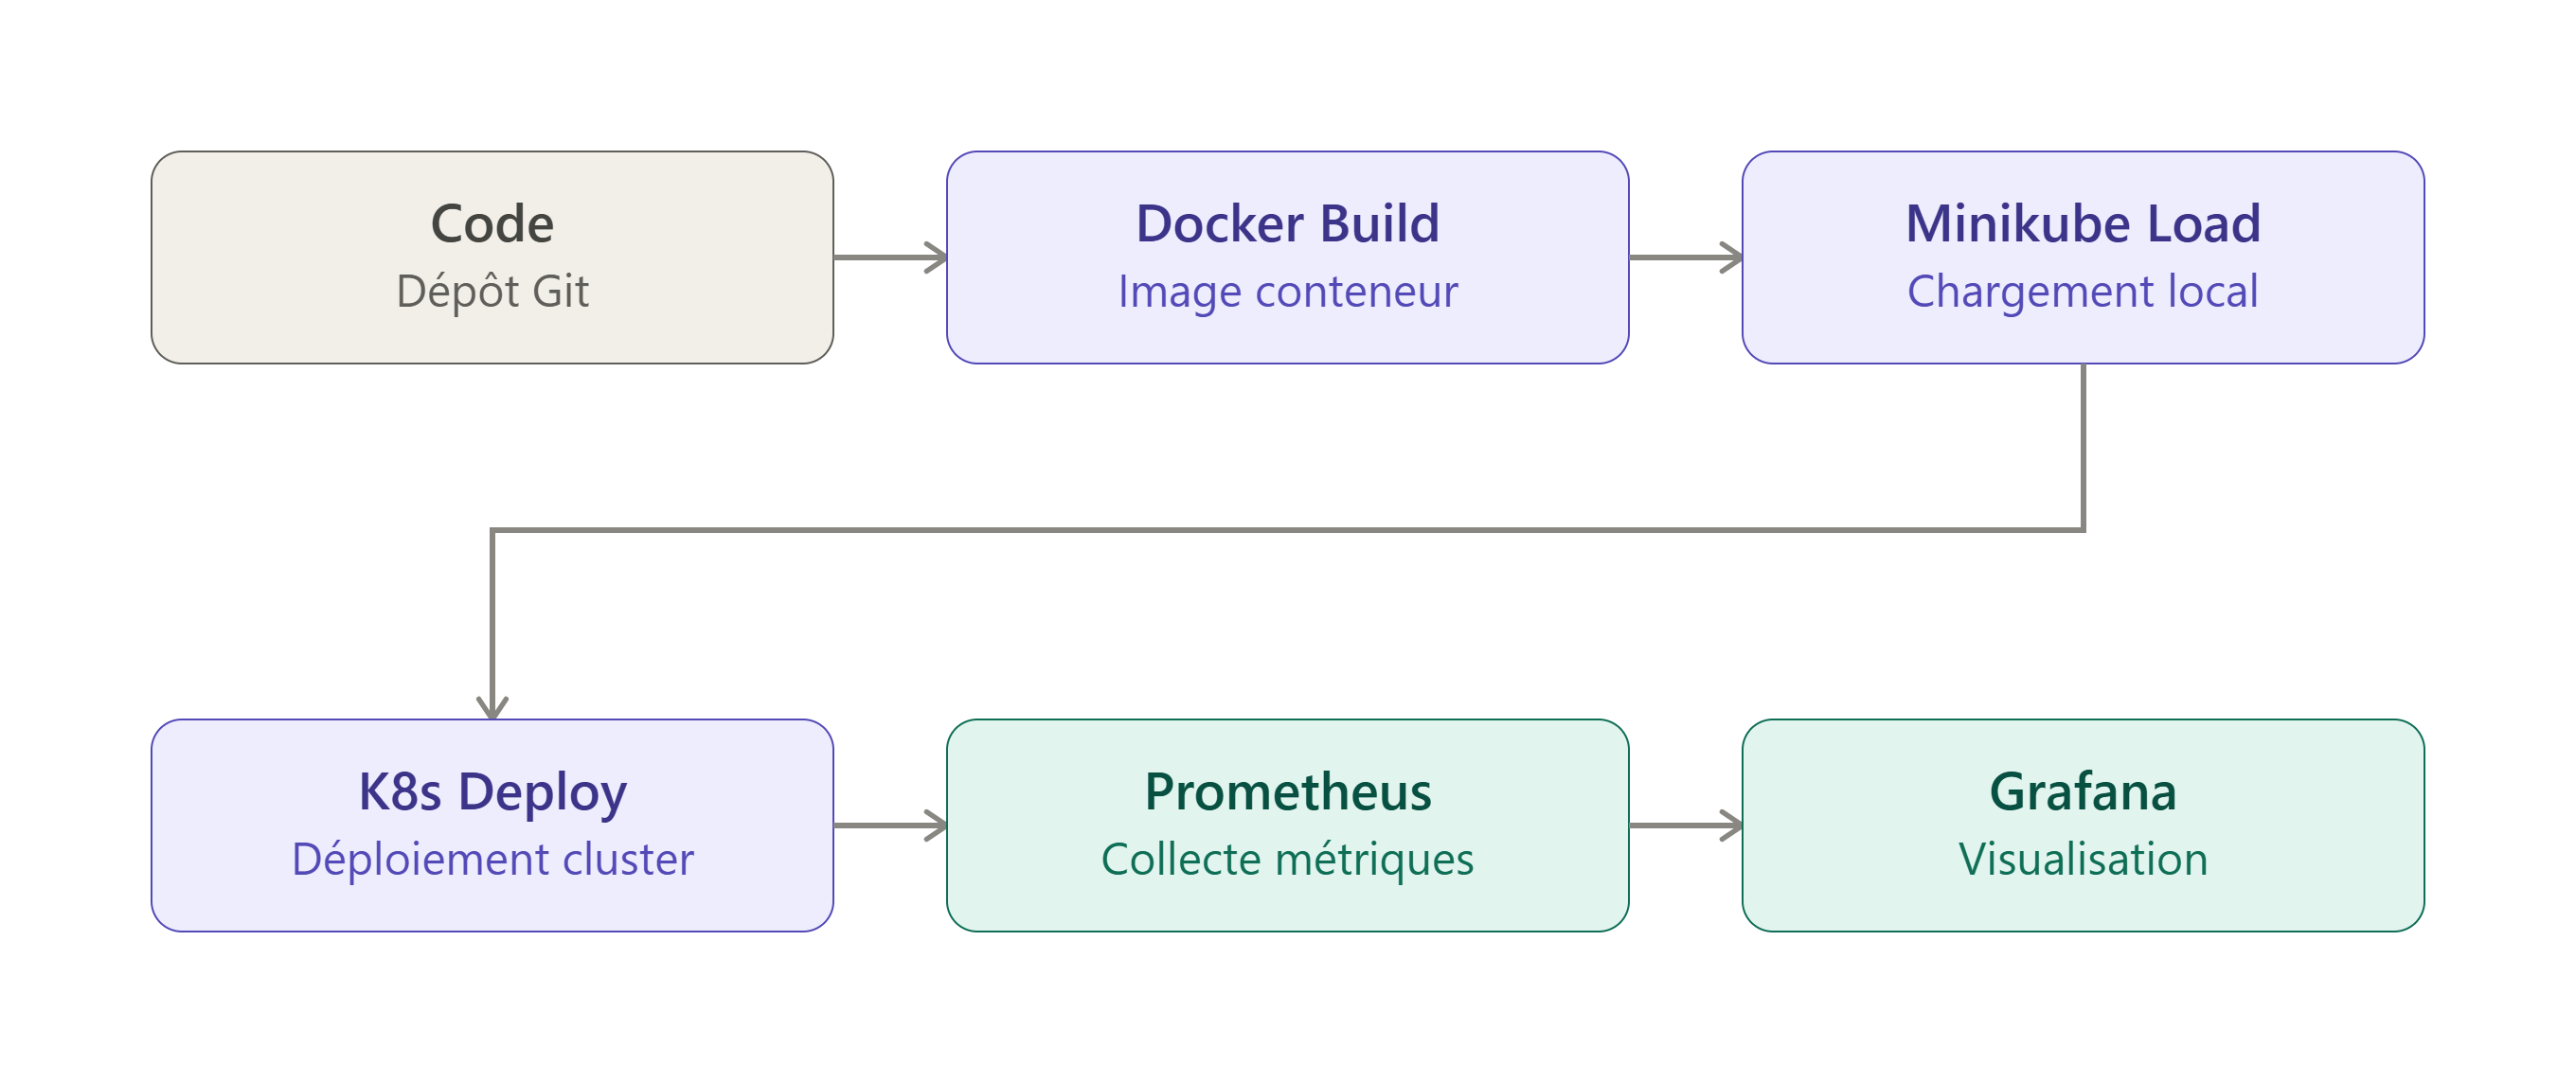
\includegraphics[width=\textwidth]{images/pipeline_devops.png}
  \caption{Pipeline DevOps de SmartPM}
  \label{fig:pipeline_devops}
\end{figure}

\subsection{Architecture Kubernetes}

Le cluster Kubernetes de SmartPM est composé de \textbf{6 deployments} interconnectés,
couvrant l'ensemble des besoins applicatifs et opérationnels de la plateforme.

\begin{table}[H]
  \centering
  \caption{Architecture Kubernetes — Pods et services de SmartPM}
  \label{tab:k8s}
  \renewcommand{\arraystretch}{1.4}
  \begin{tabularx}{\textwidth}{|l|l|l|X|}
    \hline
    \rowcolor{tablehead}
    \textcolor{white}{\textbf{Service}} &
    \textcolor{white}{\textbf{Image}} &
    \textcolor{white}{\textbf{NodePort}} &
    \textcolor{white}{\textbf{Rôle}} \\
    \hline
    Frontend & smartpm-frontend & 30080 & Interface Angular servie par Nginx \\
    \hline
    Backend & smartpm-backend & 30000 & API REST NestJS \\
    \hline
    AI Service & smartpm-ai & 30800 & Chatbot FastAPI + LLM streaming \\
    \hline
    MongoDB & mongo & — & Base de données (remplacé par Atlas en prod) \\
    \hline
    Prometheus & prom/prometheus & 30900 & Collecte de métriques \\
    \hline
    Grafana & grafana/grafana & 30300 & Dashboards de monitoring \\
    \hline
  \end{tabularx}
\end{table}

\begin{figure}[H]
  \centering
  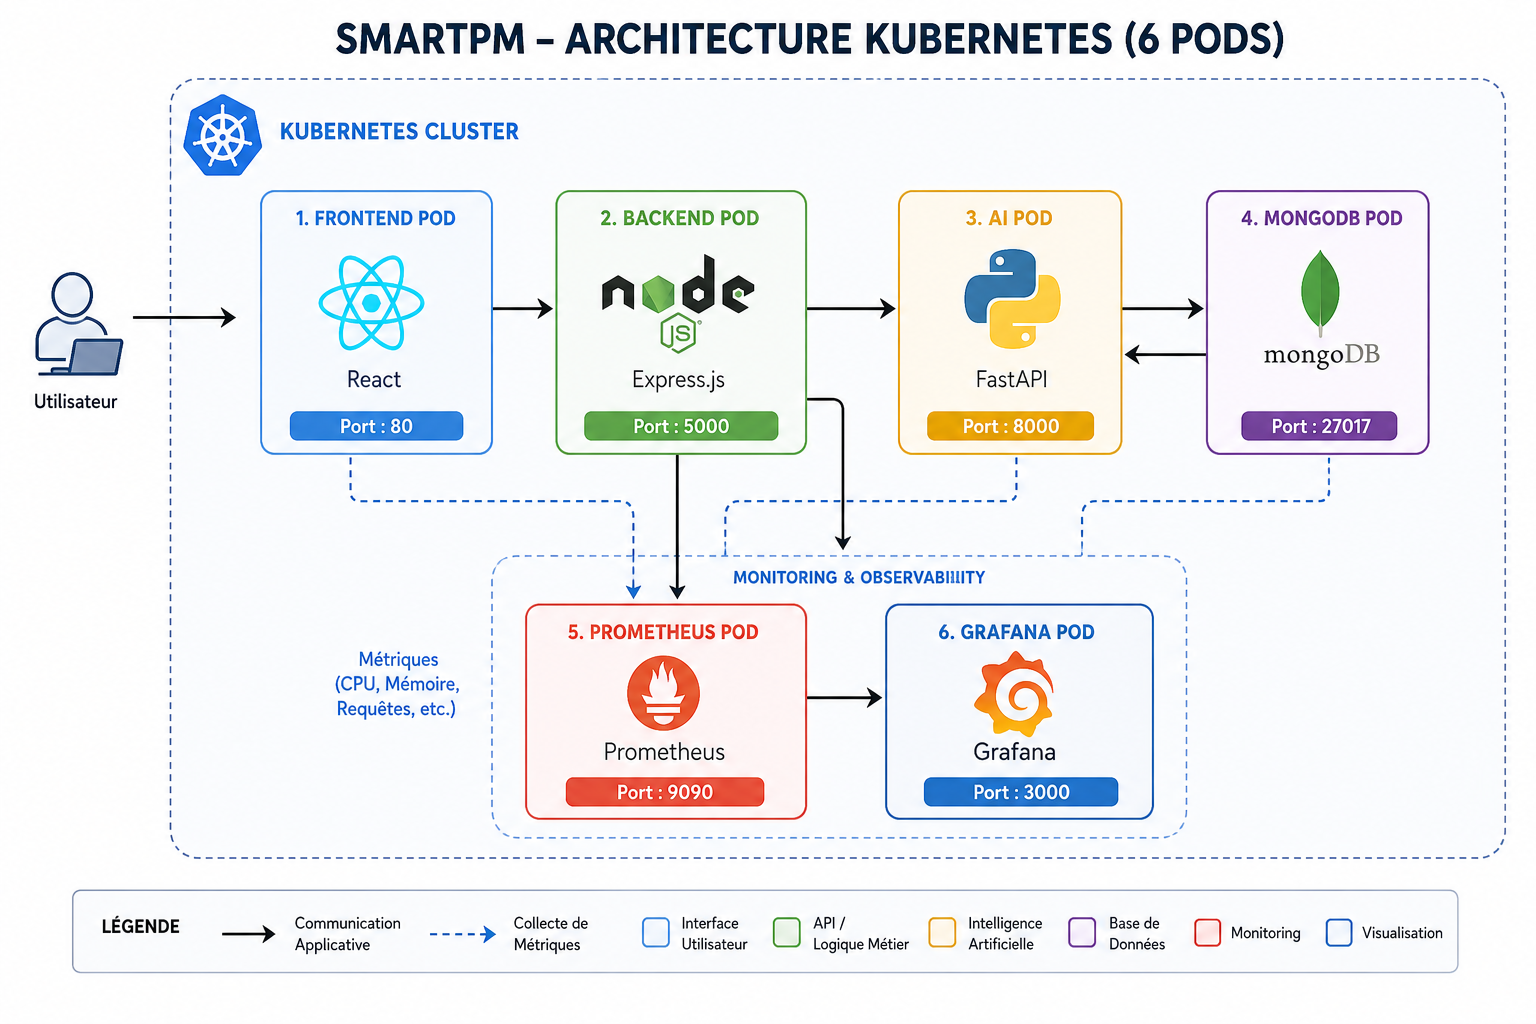
\includegraphics[width=\textwidth]{images/architecture_k8s.png}
  \caption{Architecture Kubernetes complète de SmartPM}
  \label{fig:archi_k8s}
\end{figure}


% ─────────────────────────────────────────────────────────
\section*{Conclusion}
% ─────────────────────────────────────────────────────────

Ce chapitre nous a permis de définir avec précision les besoins fonctionnels et non
fonctionnels de SmartPM, d'identifier les acteurs du système et de structurer le backlog
produit selon la méthodologie Scrum. Nous avons également présenté l'architecture technique
retenue — physique, logicielle et IA — ainsi que les choix technologiques justifiés et la
solution DevOps sur Kubernetes.

\vspace{0.3cm}

Le chapitre suivant sera consacré à la première release du projet, couvrant les sprints~1,
2 et~3, qui constituent le socle fonctionnel de la plateforme SmartPM.

% ============================================================
%  CHAPITRE 3 — RELEASE 1 : SOCLE FONCTIONNEL DE SMARTPM
% ============================================================
\chapter{Release 1 : Mise en place du socle fonctionnel de SmartPM}

\vspace{-0.3cm}
\begin{tcolorbox}[colback=lightgray, colframe=primaryblue,
  title=\textbf{Plan}, fonttitle=\bfseries]
  \begin{enumerate}[leftmargin=*, label=\arabic*.]
    \item Sprint 1 --- Authentification \& Gestion des utilisateurs
    \item Sprint 2 --- Gestion des projets \& Hi\'erarchie des t\^aches
    \item Sprint 3 --- Revues, Commentaires \& Notifications
  \end{enumerate}
\end{tcolorbox}

% ─────────────────────────────────────────────────────────
\section*{Introduction}
% ─────────────────────────────────────────────────────────

La premi\`ere release de SmartPM constitue le fondement sur lequel repose
l'ensemble de la plateforme. Elle a pour objectif d'\'etablir un socle
fonctionnel solide, s\'ecuris\'e et conforme aux exigences du d\'eveloppement
logiciel critique. Cette release couvre trois sprints d'une dur\'ee totale de
six semaines.

\vspace{0.3cm}

Pour chaque sprint, nous pr\'esenterons les objectifs, le backlog, la
sp\'ecification des besoins via un diagramme de cas d'utilisation, le
diagramme de classes, les diagrammes dynamiques (s\'equence, activit\'e,
\'etat), puis les interfaces r\'ealis\'ees.

% ═══════════════════════════════════════════════════════════
\newpage
\section{Sprint 1 : Authentification \& Gestion des utilisateurs}
\label{sec:s1}
% ═══════════════════════════════════════════════════════════

Ce premier sprint est consacr\'e \`a la mise en place de l'infrastructure
de s\'ecurit\'e et de gestion des identit\'es de SmartPM. Il constitue le
pr\'erequis indispensable de toutes les fonctionnalit\'es ult\'erieures.

\subsection{Objectifs du sprint 1}

L'objectif principal de ce sprint est de d\'evelopper un syst\`eme
d'authentification robuste et multi-m\'ethodes. Plus pr\'ecis\'ement, il
s'agit de :

\begin{itemize}
  \item Int\'egrer un syst\`eme d'authentification par tokens JWT
        (\textit{JSON Web Token}) avec gestion du refresh token (validit\'e
        15 minutes pour l'access token, 7 jours pour le refresh token).
  \item Impl\'ementer le protocole OAuth2 pour la connexion sociale
        via Google et GitHub.
  \item D\'efinir et appliquer une gestion fine des r\^oles utilisateurs :
        \textbf{ADMIN}, \textbf{MANAGER} et \textbf{MEMBER}.
  \item Mettre en place un seedage automatique du compte administrateur
        au premier d\'emarrage du backend (via \texttt{OnApplicationBootstrap}).
  \item D\'evelopper le module d'administration : CRUD complet sur les
        utilisateurs, consultation des journaux d'audit et r\'einitialisation
        des mots de passe.
\end{itemize}

\subsection{Backlog du sprint 1}

Le tableau~\ref{tab:backlog_s1} pr\'esente le backlog d\'etaill\'e du premier sprint.

\begin{table}[H]
\centering
\renewcommand{\arraystretch}{1.4}
\begin{tabularx}{\textwidth}{|c|X|c|c|}
\hline
\rowcolor{tablehead}
\textcolor{white}{\textbf{ID}} &
\textcolor{white}{\textbf{User Story}} &
\textcolor{white}{\textbf{Priorit\'e}} &
\textcolor{white}{\textbf{Charge (j)}} \\ \hline
US-1.1 & En tant qu'utilisateur, je peux m'inscrire avec email et mot de passe & Haute & 2 \\ \hline
US-1.2 & En tant qu'utilisateur, je peux me connecter via JWT (Login) & Haute & 2 \\ \hline
US-1.3 & En tant qu'utilisateur, je renouvelle mon token via le refresh token & Haute & 1 \\ \hline
US-1.4 & En tant qu'utilisateur, je me connecte via Google OAuth2 & Haute & 2 \\ \hline
US-1.5 & En tant qu'utilisateur, je me connecte via GitHub OAuth2 & Haute & 1 \\ \hline
US-1.6 & Le compte Admin est cr\'e\'e automatiquement au d\'emarrage & Haute & 1 \\ \hline
US-1.7 & En tant qu'Admin, je g\`ere les comptes utilisateurs (CRUD) & Moyenne & 3 \\ \hline
US-1.8 & En tant qu'Admin, je consulte les journaux d'audit & Moyenne & 2 \\ \hline
US-1.9 & En tant qu'Admin, je r\'einitialise le mot de passe d'un utilisateur & Faible & 1 \\ \hline
\end{tabularx}
\caption{Backlog du Sprint 1 --- Authentification \& Gestion des utilisateurs}
\label{tab:backlog_s1}
\end{table}

\subsection{Sp\'ecification des besoins fonctionnels}

\subsubsection{Identification des acteurs}

Trois acteurs interagissent avec le sous-syst\`eme d'authentification :
l'\textbf{Utilisateur non authentifi\'e} (peut s'inscrire et se connecter),
l'\textbf{Utilisateur authentifi\'e} (peut renouveler son token et se
d\'econnecter) et l'\textbf{Administrateur} (h\'erite des droits utilisateur
et dispose des fonctions d'administration).

\subsubsection{Diagramme de cas d'utilisation}

La figure~\ref{fig:uc_s1} repr\'esente les interactions entre les acteurs
et le sous-syst\`eme d'authentification de SmartPM.

\begin{figure}[H]
  \centering
  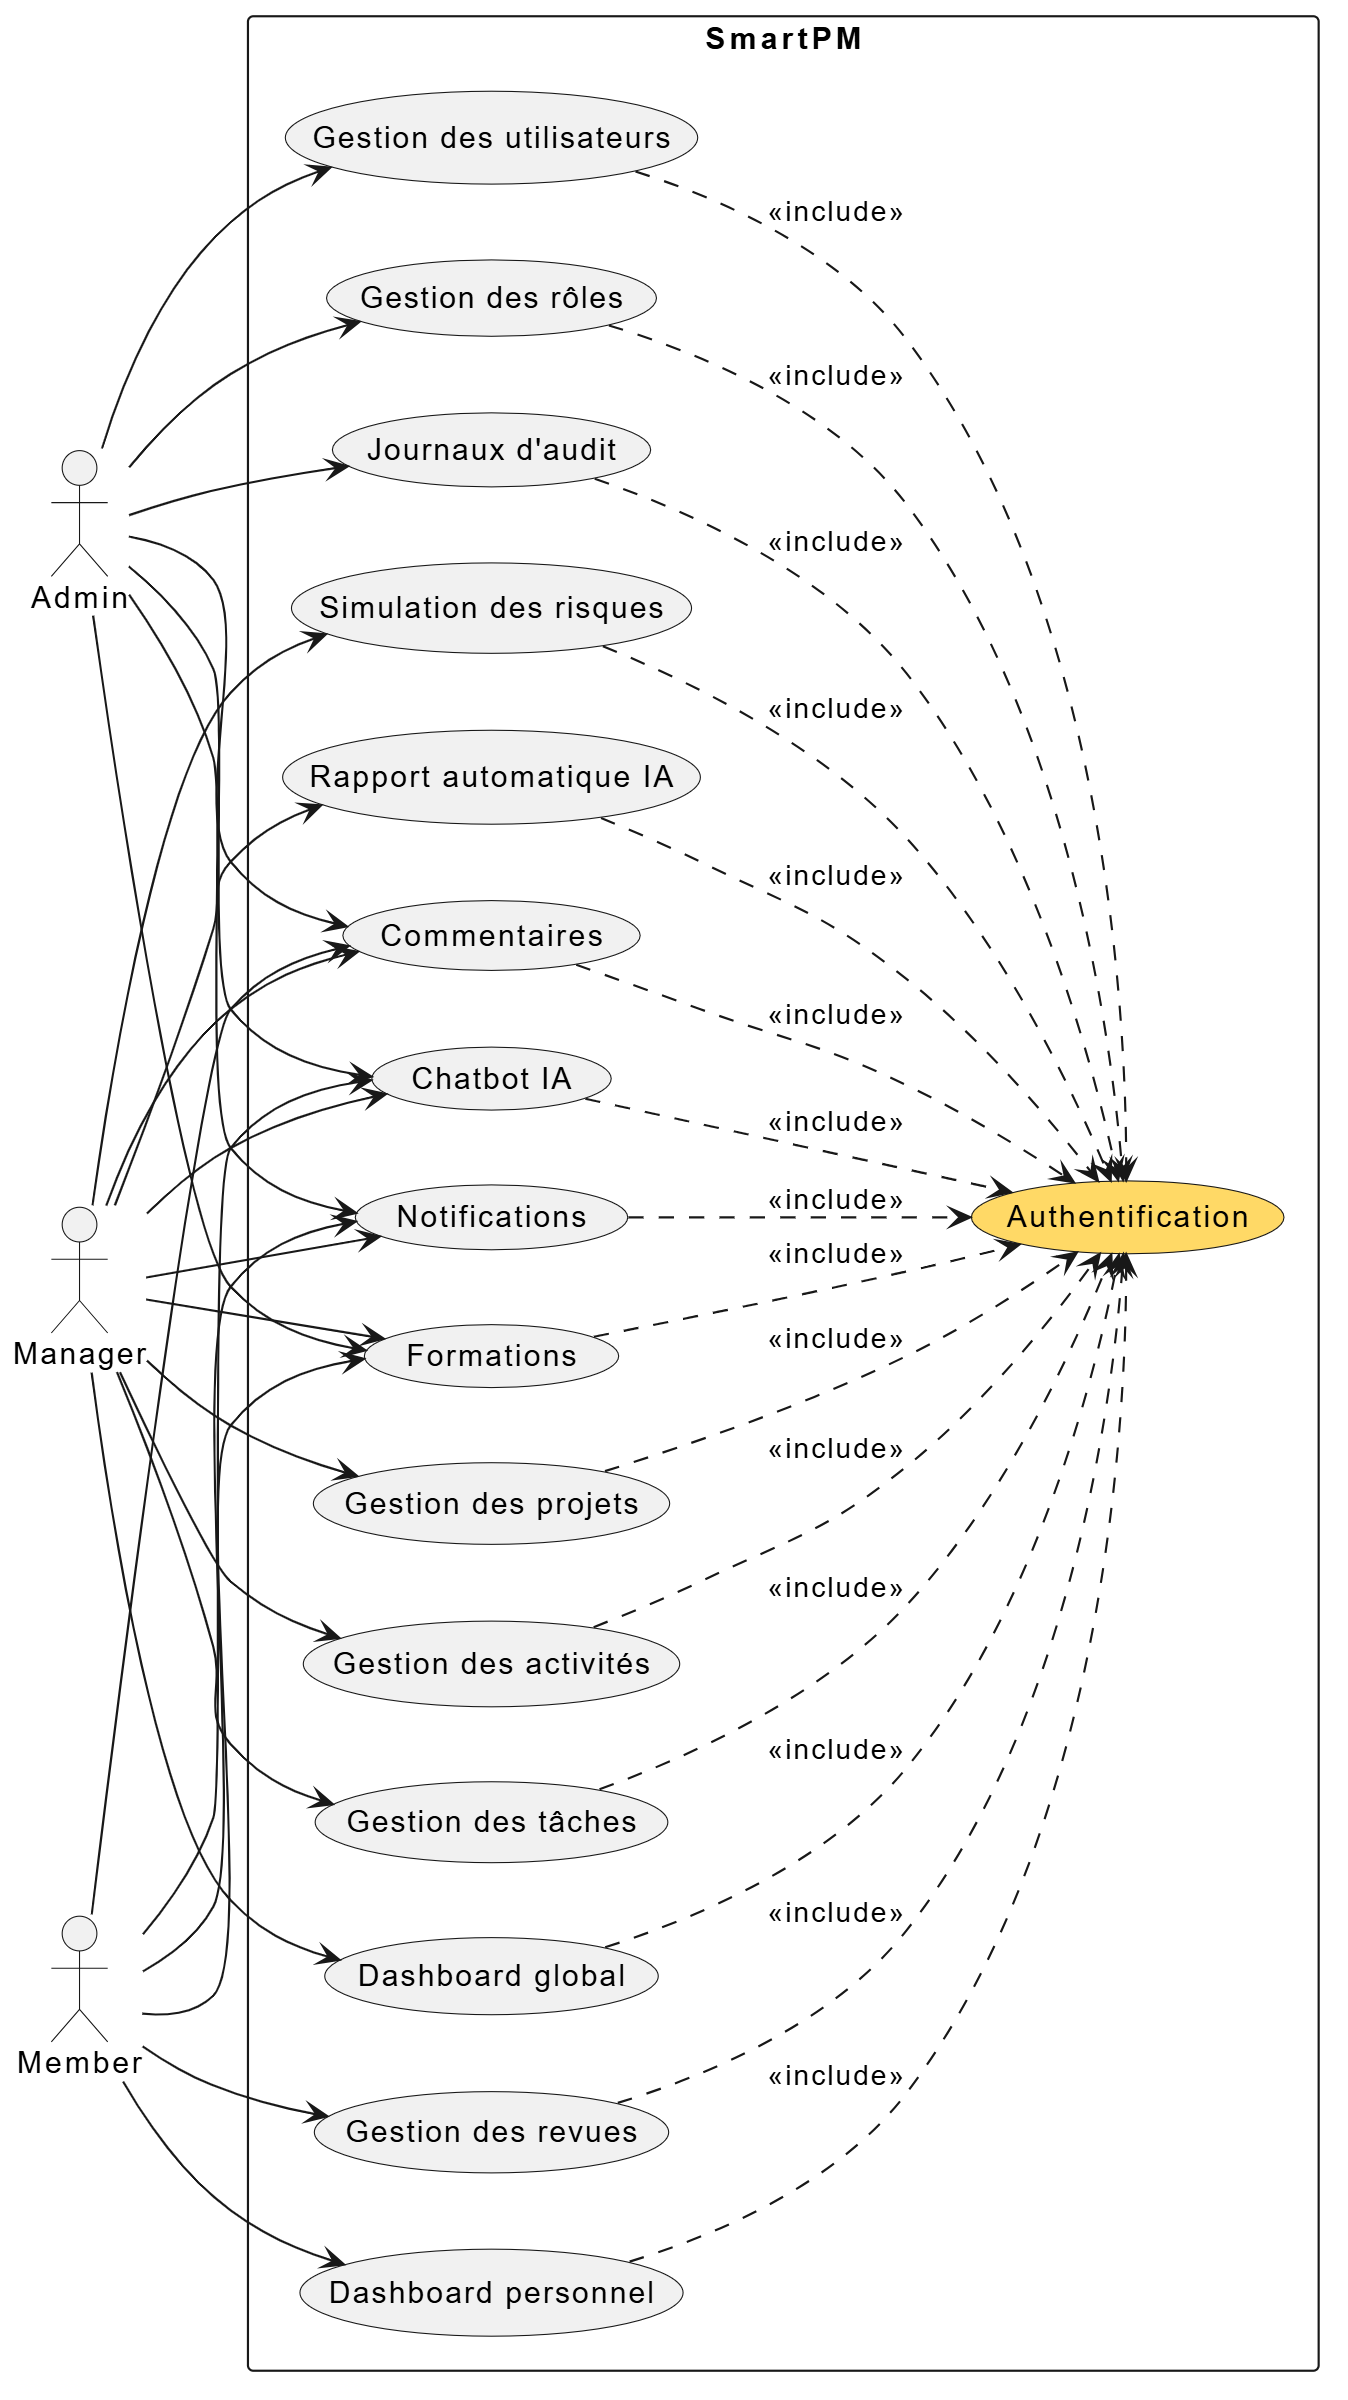
\includegraphics[width=\textwidth]{figures/chapter3/sprint1/uc_sprint1.png}
  \caption{Diagramme de cas d'utilisation --- Sprint 1}
  \label{fig:uc_s1}
\end{figure}

\subsection{Diagramme de classes du sprint 1}

La figure~\ref{fig:class_s1} pr\'esente le diagramme de classes du sprint 1.
Les entit\'es principales sont : \textbf{User} (email, passwordHash, role,
status, isOAuthUser), \textbf{RefreshToken} (token, userId, expiresAt,
isRevoked) et \textbf{AuditLog} (actorId, action, targetId, createdAt).

\begin{figure}[H]
  \centering
  \includegraphics[width=\textwidth]{figures/chapter3/sprint1/class_sprint1.png}
  \caption{Diagramme de classes --- Sprint 1}
  \label{fig:class_s1}
\end{figure}

\subsection{Diagrammes dynamiques du sprint 1}

\subsubsection{Diagramme de s\'equence --- Authentification JWT}

Le diagramme~\ref{fig:seq_jwt} illustre le flux complet d'authentification
par token JWT. L'utilisateur soumet son email et mot de passe depuis le
composant Angular \texttt{LoginComponent}. Le backend NestJS valide les
identifiants via la strat\'egie \texttt{LocalStrategy} de Passport.js,
compare le mot de passe avec le hash bcrypt stock\'e en base, puis g\'en\`ere
un access token (15 minutes) et un refresh token (7 jours). Le refresh token
est persist\'e dans MongoDB Atlas. Les requ\^etes ult\'erieures includent
l'access token dans l'en-t\^ete \texttt{Authorization: Bearer <token>}
inject\'e par un \texttt{HttpInterceptor} Angular.

\begin{figure}[H]
  \centering
  \includegraphics[width=\textwidth]{figures/chapter3/sprint1/seq_jwt.png}
  \caption{Diagramme de s\'equence --- Authentification JWT}
  \label{fig:seq_jwt}
\end{figure}

\subsubsection{Diagramme de s\'equence --- OAuth2 Social Login}

Le diagramme~\ref{fig:seq_oauth} illustre le flux d'autorisation OAuth2
(\textit{Authorization Code Flow}). Ce flux garantit que les identifiants
de l'utilisateur ne transitent jamais par le backend SmartPM. Apr\`es
redirection vers le fournisseur (Google ou GitHub), le profil r\'ecup\'er\'e
est upsert\'e dans MongoDB Atlas et un JWT SmartPM est g\'en\'er\'e.

\begin{figure}[H]
  \centering
  \includegraphics[width=\textwidth]{figures/chapter3/sprint1/seq_oauth2.png}
  \caption{Diagramme de s\'equence --- OAuth2 Social Login (Google / GitHub)}
  \label{fig:seq_oauth}
\end{figure}

\subsection{R\'ealisation du sprint 1}

\subsubsection{Architecture du module d'authentification}

Trois modules NestJS ont \'et\'e cr\'e\'es pour ce sprint :
\textbf{AuthModule} (orchestration JWT + OAuth2, endpoints
\texttt{/auth/login}, \texttt{/auth/register}, \texttt{/auth/refresh}),
\textbf{UserModule} (CRUD utilisateurs, sch\'ema Mongoose avec validation)
et \textbf{AdminModule} (prot\'eg\'e par \texttt{JwtAuthGuard} +
\texttt{RolesGuard(ADMIN)}, CRUD + audit logs).

\vspace{0.3cm}

Les mots de passe sont hash\'es avec \textbf{bcrypt} (facteur de co\^ut 12).
Trois strat\'egies Passport.js ont \'et\'e impl\'ement\'ees :
\texttt{LocalStrategy} (email/mot de passe), \texttt{JwtStrategy}
(v\'erification des tokens) et \texttt{GoogleStrategy}/\texttt{GitHubStrategy}
(OAuth2).

\subsubsection{Interfaces r\'ealis\'ees}

\begin{figure}[H]
  \centering
  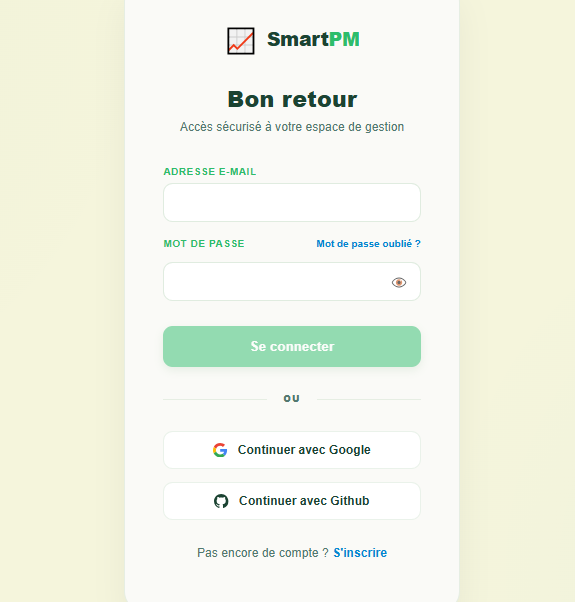
\includegraphics[width=0.8\textwidth]{images/screen_login.png}
  \caption{Interface de connexion de SmartPM}
  \label{fig:scr_login}
\end{figure}

\begin{figure}[H]
  \centering
  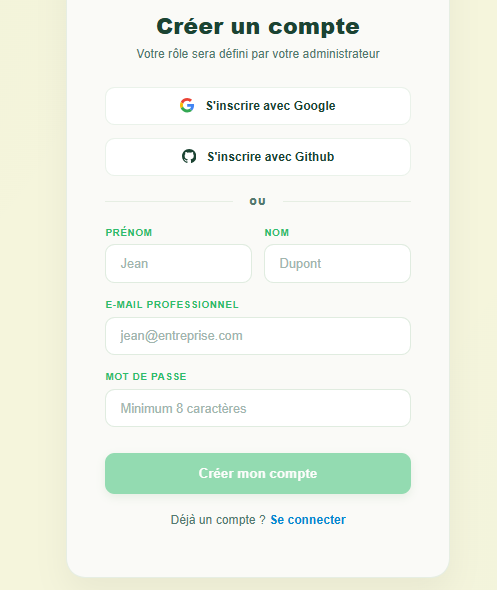
\includegraphics[width=0.8\textwidth]{images/screen_register.png}
  \caption{Interface d'inscription de SmartPM}
  \label{fig:scr_register}
\end{figure}

\begin{figure}[H]
  \centering
  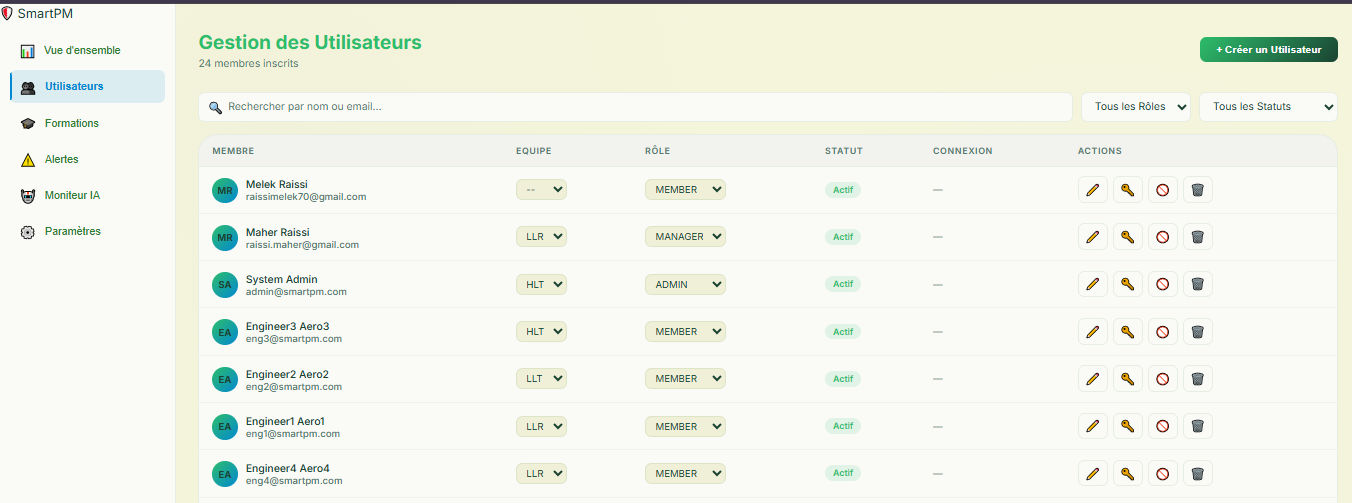
\includegraphics[width=\textwidth]{images/screen_admin_users.png}
  \caption{Module Admin --- Gestion des utilisateurs}
  \label{fig:scr_admin}
\end{figure}

\begin{figure}[H]
  \centering
  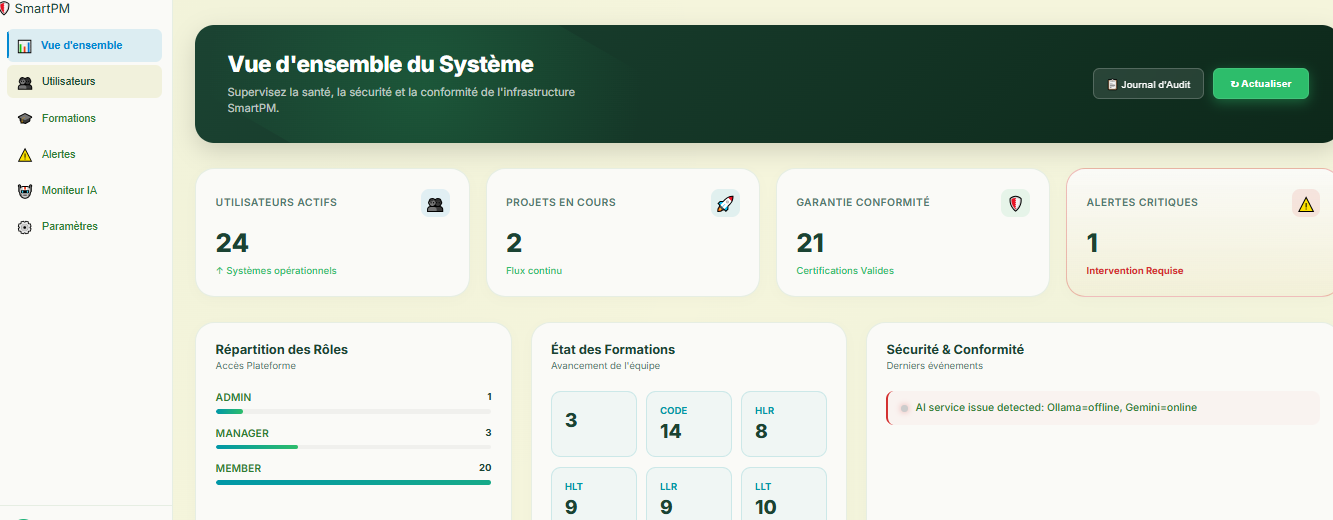
\includegraphics[width=\textwidth]{images/screen_audit_logs.png}
  \caption{Module Admin --- Journal d'audit des actions}
  \label{fig:scr_audit}
\end{figure}

% ═══════════════════════════════════════════════════════════
\newpage
\section{Sprint 2 : Gestion des projets \& Hi\'erarchie des t\^aches}
\label{sec:s2}
% ═══════════════════════════════════════════════════════════

Ce deuxi\`eme sprint constitue le c\oe ur m\'etier de SmartPM.
Il impl\'emente la structure de donn\'ees a\'eronautique conforme \`a
la norme DO-178C, qui impose une d\'ecomposition stricte du travail
en niveaux hi\'erarchiques.

\subsection{Objectifs du sprint 2}

\begin{itemize}
  \item Impl\'ementer le CRUD complet des projets avec un wizard
        multi-\'etapes (5 \'etapes).
  \item Mettre en place la hi\'erarchie \`a quatre niveaux :
        \textbf{Projet} $\rightarrow$ \textbf{Activit\'e} $\rightarrow$
        \textbf{Sous-Activit\'e} $\rightarrow$ \textbf{T\^ache}.
  \item G\'erer l'affectation des \'equipes et des membres aux projets.
  \item Impl\'ementer les \textit{Function Templates} (mod\`eles r\'eutilisables).
  \item D\'evelopper les tableaux de bord Manager et Member.
\end{itemize}

\subsection{Backlog du sprint 2}

\begin{table}[H]
\centering
\renewcommand{\arraystretch}{1.4}
\begin{tabularx}{\textwidth}{|c|X|c|c|}
\hline
\rowcolor{tablehead}
\textcolor{white}{\textbf{ID}} &
\textcolor{white}{\textbf{User Story}} &
\textcolor{white}{\textbf{Priorit\'e}} &
\textcolor{white}{\textbf{Charge (j)}} \\ \hline
US-2.1 & Manager : cr\'eer un projet (nom, description, dates, DAL) & Haute & 3 \\ \hline
US-2.2 & Manager : wizard multi-\'etapes de cr\'eation de projet & Haute & 4 \\ \hline
US-2.3 & Manager : CRUD des activit\'es d'un projet & Haute & 2 \\ \hline
US-2.4 & Manager : CRUD des sous-activit\'es & Haute & 2 \\ \hline
US-2.5 & Manager : CRUD des t\^aches avec affectation \`a un membre & Haute & 3 \\ \hline
US-2.6 & Manager : affecter une \'equipe \`a un projet & Haute & 2 \\ \hline
US-2.7 & Manager : cr\'eer et r\'eutiliser des Function Templates & Moyenne & 2 \\ \hline
US-2.8 & Manager : consulter le tableau de bord global & Haute & 3 \\ \hline
US-2.9 & Member : consulter son tableau de bord personnel & Haute & 2 \\ \hline
US-2.10 & Member : mettre \`a jour le statut d'une t\^ache & Haute & 1 \\ \hline
\end{tabularx}
\caption{Backlog du Sprint 2 --- Gestion des projets \& Hi\'erarchie des t\^aches}
\label{tab:backlog_s2}
\end{table}

\subsection{Sp\'ecification des besoins fonctionnels}

\subsubsection{Hi\'erarchie DO-178C dans SmartPM}

La norme DO-178C structure le d\'eveloppement logiciel en phases successives.
SmartPM traduit cette structure en quatre niveaux hi\'erarchiques :

\begin{itemize}
  \item \textbf{Projet} : Entit\'e racine repr\'esentant un programme
        logiciel a\'eronautique, associ\'e \`a une norme (DO-178C/DO-254)
        et un niveau de criticit\'e DAL (A \`a E).
  \item \textbf{Activit\'e} : Correspond \`a une phase majeure du cycle
        de vie (Requirements, Design, Coding, Testing).
  \item \textbf{Sous-Activit\'e} : D\'ecompose une activit\'e en travaux
        plus fins assignables \`a des individus sp\'ecifiques.
  \item \textbf{T\^ache} : Unit\'e atomique de travail, assign\'ee \`a un
        membre avec statut \texttt{TODO} $\rightarrow$ \texttt{IN\_PROGRESS}
        $\rightarrow$ \texttt{IN\_REVIEW} $\rightarrow$ \texttt{DONE}.
\end{itemize}

\subsubsection{Diagramme de cas d'utilisation}

\begin{figure}[H]
  \centering
  \includegraphics[width=\textwidth]{figures/chapter3/sprint2/uc_sprint2.png}
  \caption{Diagramme de cas d'utilisation --- Sprint 2}
  \label{fig:uc_s2}
\end{figure}

\subsection{Diagramme de classes du sprint 2}

La figure~\ref{fig:class_s2} pr\'esente le mod\`ele de donn\'ees du
sprint 2 : \textbf{Project} (m\'etadonn\'ees, DAL, norme),
\textbf{Team} (liste des membres), \textbf{Activity}, \textbf{SubActivity},
\textbf{Task} (assigneeId, status, priority, dueDate) et
\textbf{FunctionTemplate} (mod\`ele r\'eutilisable).

\begin{figure}[H]
  \centering
  \includegraphics[width=\textwidth]{figures/chapter3/sprint2/class_sprint2.png}
  \caption{Diagramme de classes --- Sprint 2}
  \label{fig:class_s2}
\end{figure}

\subsection{Diagrammes dynamiques du sprint 2}

\subsubsection{Diagramme de s\'equence --- Wizard de cr\'eation de projet}

Le \textit{Project Wizard} guide le Manager en 5 \'etapes :
(1)~Informations g\'en\'erales, (2)~Configuration normative (DAL, norme),
(3)~Structure des activit\'es, (4)~Constitution de l'\'equipe,
(5)~Confirmation. \`A l'\'etape finale, un \texttt{POST /projects} cr\'ee
le projet, ses activit\'es et affecte l'\'equipe en cascade.

\begin{figure}[H]
  \centering
  \includegraphics[width=\textwidth]{figures/chapter3/sprint2/seq_wizard.png}
  \caption{Diagramme de s\'equence --- Wizard de cr\'eation de projet}
  \label{fig:seq_wiz}
\end{figure}

\subsubsection{Diagramme d'activit\'e --- Cycle de vie d'une t\^ache}

\begin{figure}[H]
  \centering
  \includegraphics[width=\textwidth]{figures/chapter3/sprint2/activity_task.png}
  \caption{Diagramme d'activit\'e --- Cycle de vie d'une t\^ache}
  \label{fig:act_task}
\end{figure}

\subsection{R\'ealisation du sprint 2}

Cinq modules NestJS ont \'et\'e d\'evelopp\'es pour ce sprint :
\textbf{ProjectModule}, \textbf{ActivityModule}, \textbf{SubActivityModule},
\textbf{TaskModule} et \textbf{FunctionTemplateModule}. C\^ot\'e frontend,
quatre composants Angular ont \'et\'e cr\'e\'es :
\texttt{ProjectWizardComponent}, \texttt{ProjectDetailComponent},
\texttt{ManagerDashboardComponent} et \texttt{MemberDashboardComponent}.

\begin{figure}[H]
  \centering
  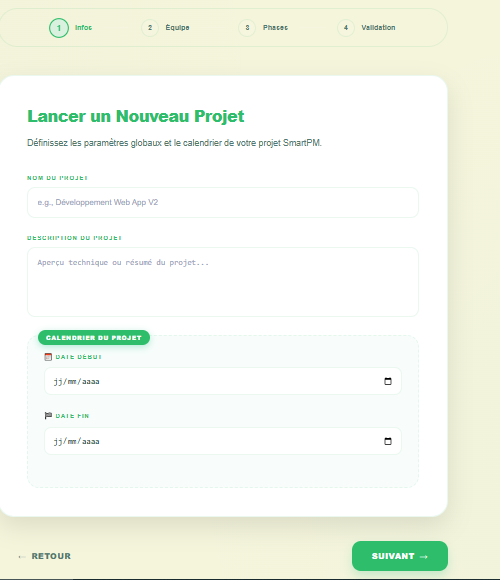
\includegraphics[width=0.85\textwidth]{images/screen_wizard_step1.png}
  \caption{Project Wizard --- \'Etape 1 : Informations g\'en\'erales}
  \label{fig:scr_wiz1}
\end{figure}

\begin{figure}[H]
  \centering
  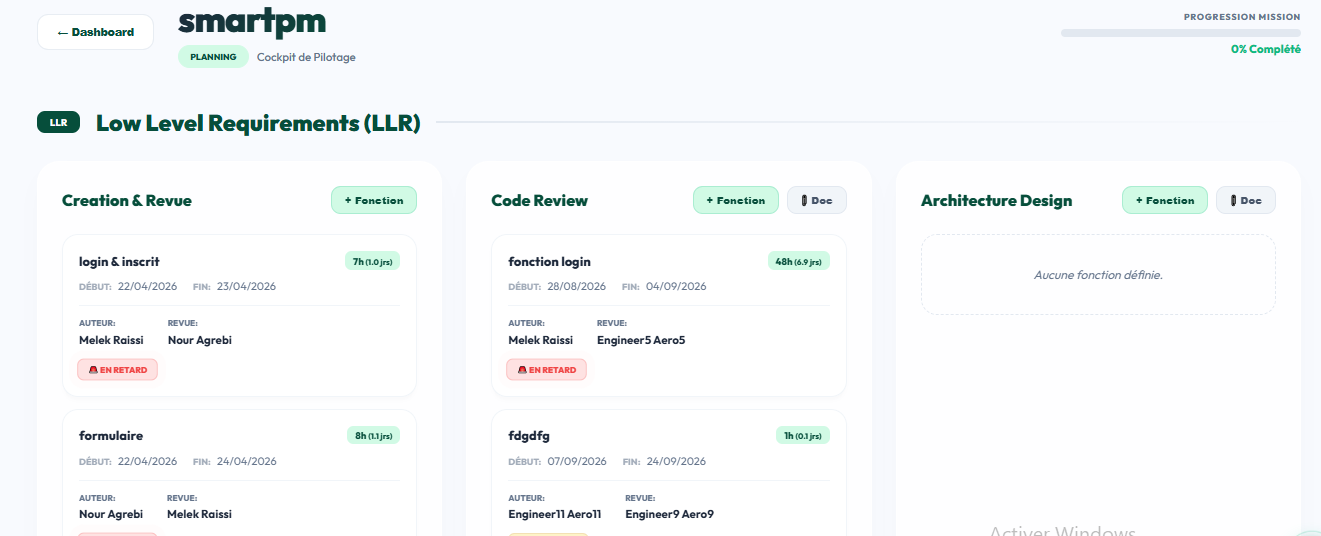
\includegraphics[width=\textwidth]{images/screen_project_detail.png}
  \caption{Vue d\'etaill\'ee d'un projet a\'eronautique SmartPM}
  \label{fig:scr_proj}
\end{figure}

\begin{figure}[H]
  \centering
  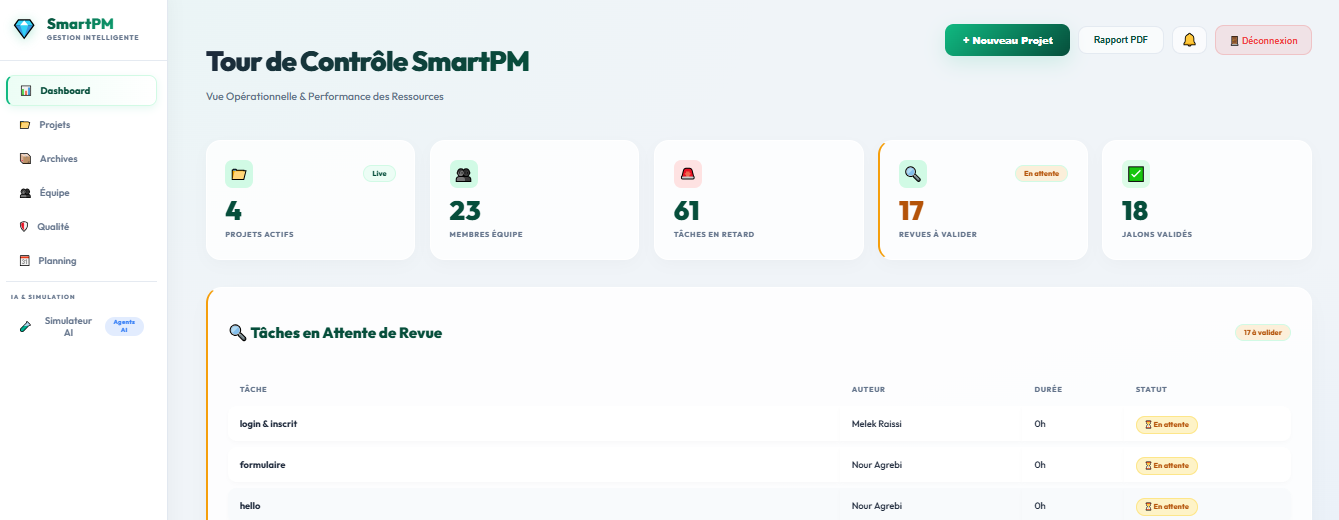
\includegraphics[width=\textwidth]{images/screen_manager_dashboard.png}
  \caption{Tableau de bord Manager --- Vue globale des projets}
  \label{fig:scr_mgr}
\end{figure}

\begin{figure}[H]
  \centering
  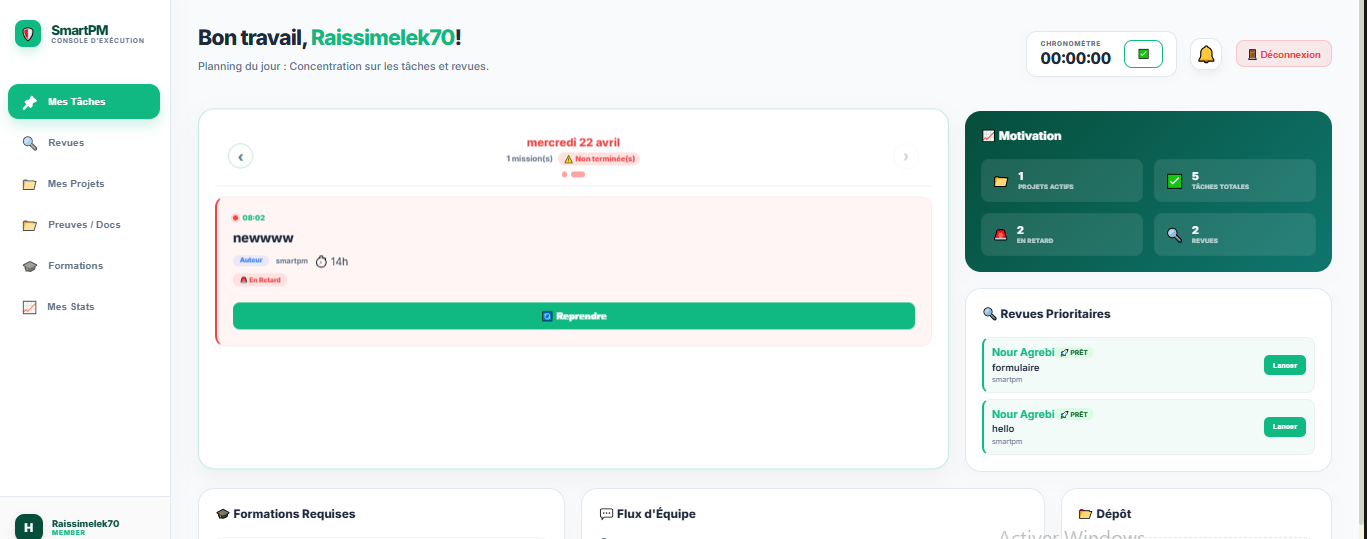
\includegraphics[width=\textwidth]{images/screen_member_dashboard.png}
  \caption{Tableau de bord Membre --- Vue personnelle des t\^aches}
  \label{fig:scr_mbr}
\end{figure}

% ═══════════════════════════════════════════════════════════
\newpage
\section{Sprint 3 : Revues, Commentaires \& Notifications}
\label{sec:s3}
% ═══════════════════════════════════════════════════════════

Ce troisi\`eme sprint enrichit SmartPM de m\'ecanismes de collaboration
et de contr\^ole qualit\'e conformes aux exigences DO-178C. La norme impose
que toute t\^ache soit r\'evis\'ee par une personne diff\'erente de son
auteur (\textbf{Author $\neq$ Reviewer}).

\subsection{Objectifs du sprint 3}

\begin{itemize}
  \item Impl\'ementer un syst\`eme de revues formelles avec la contrainte
        \textbf{Author $\neq$ Reviewer} (exigence DO-178C \S6.3).
  \item G\'erer le cycle de vie complet d'une revue :
        \texttt{PENDING} $\rightarrow$ \texttt{IN\_REVIEW} $\rightarrow$
        \texttt{APPROVED} ou \texttt{CHANGES\_REQUESTED}.
  \item Permettre aux membres de commenter les t\^aches (fil de discussion).
  \item Mettre en place des notifications en temps r\'eel via WebSockets.
  \item Impl\'ementer le suivi des certifications par phase DO-178C :
        HLR, LLR, CODE, LLT, HLT.
\end{itemize}

\subsection{Backlog du sprint 3}

\begin{table}[H]
\centering
\renewcommand{\arraystretch}{1.4}
\begin{tabularx}{\textwidth}{|c|X|c|c|}
\hline
\rowcolor{tablehead}
\textcolor{white}{\textbf{ID}} &
\textcolor{white}{\textbf{User Story}} &
\textcolor{white}{\textbf{Priorit\'e}} &
\textcolor{white}{\textbf{Charge (j)}} \\ \hline
US-3.1 & Member : soumettre une t\^ache \`a revue (Author $\neq$ Reviewer) & Haute & 3 \\ \hline
US-3.2 & Reviewer : approuver ou rejeter une revue avec commentaire & Haute & 2 \\ \hline
US-3.3 & Member : voir la liste des revues en attente & Haute & 1 \\ \hline
US-3.4 & Member : commenter une t\^ache (fil de discussion) & Moyenne & 2 \\ \hline
US-3.5 & Utilisateur : recevoir des notifications en temps r\'eel (WebSocket) & Haute & 3 \\ \hline
US-3.6 & Manager : valider une certification de phase (HLR/LLR/CODE/LLT/HLT) & Haute & 3 \\ \hline
US-3.7 & Member : voir son tableau de certifications par phase & Haute & 2 \\ \hline
\end{tabularx}
\caption{Backlog du Sprint 3 --- Revues, Commentaires \& Notifications}
\label{tab:backlog_s3}
\end{table}

\subsection{Sp\'ecification des besoins fonctionnels}

\subsubsection{La contrainte Author $\neq$ Reviewer dans DO-178C}

La norme DO-178C stipule dans sa section~6.3 que les activit\'es de
v\'erification doivent \^etre ind\'ependantes du processus de d\'eveloppement.
Dans SmartPM, cette contrainte est appliqu\'ee au niveau du service :
lors de l'assignation d'un reviewer, le \texttt{ReviewService} v\'erifie
que \texttt{authorId} $\neq$ \texttt{reviewerId}. Toute tentative
d'auto-assignation retourne une erreur HTTP~409 avec le message
\textit{<<~Un auteur ne peut pas r\'eviser sa propre t\^ache (DO-178C)~>>}.

\subsubsection{Diagramme de cas d'utilisation}

\begin{figure}[H]
  \centering
  \includegraphics[width=\textwidth]{figures/chapter3/sprint3/uc_sprint3.png}
  \caption{Diagramme de cas d'utilisation --- Sprint 3}
  \label{fig:uc_s3}
\end{figure}

\subsection{Diagramme de classes du sprint 3}

\begin{figure}[H]
  \centering
  \includegraphics[width=\textwidth]{figures/chapter3/sprint3/class_sprint3.png}
  \caption{Diagramme de classes --- Sprint 3}
  \label{fig:class_s3}
\end{figure}

\subsection{Diagrammes dynamiques du sprint 3}

\subsubsection{Diagramme d'\'etat --- Cycle de vie d'une revue}

Le diagramme~\ref{fig:state_rev} illustre les transitions d'\'etat d'une
revue de t\^ache. Une revue commence dans l'\'etat \texttt{PENDING} d\`es
la soumission. Le reviewer la passe \`a \texttt{IN\_REVIEW}, puis soit
\texttt{APPROVED} (t\^ache $\rightarrow$ DONE) soit
\texttt{CHANGES\_REQUESTED} (retour \`a l'auteur pour correction).

\begin{figure}[H]
  \centering
  \includegraphics[width=\textwidth]{figures/chapter3/sprint3/state_review.png}
  \caption{Diagramme d'\'etat --- Cycle de vie d'une revue DO-178C}
  \label{fig:state_rev}
\end{figure}

\subsubsection{Diagramme de s\'equence --- Soumission et traitement d'une revue}

\begin{figure}[H]
  \centering
  \includegraphics[width=\textwidth]{figures/chapter3/sprint3/seq_review.png}
  \caption{Diagramme de s\'equence --- Soumission et traitement d'une revue}
  \label{fig:seq_rev}
\end{figure}

\subsection{R\'ealisation du sprint 3}

Quatre modules NestJS ont \'et\'e d\'evelopp\'es :
\textbf{ReviewModule} (endpoints \texttt{/reviews}, v\'erification
Author~$\neq$~Reviewer, transitions d'\'etat),
\textbf{CommentModule} (fil de discussion par t\^ache),
\textbf{NotificationModule} (\texttt{@WebSocketGateway} avec
\texttt{socket.io}, \'ev\'enements \texttt{task.assigned},
\texttt{review.requested}, \texttt{review.approved}) et
\textbf{CertificationModule} (suivi des phases HLR/LLR/CODE/LLT/HLT,
validation par Manager ou Admin).

\begin{figure}[H]
  \centering
  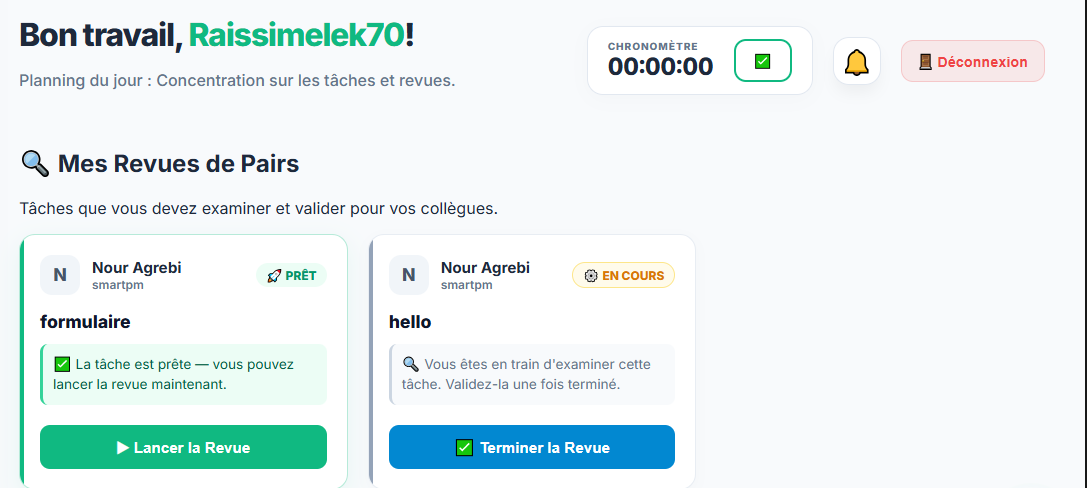
\includegraphics[width=0.85\textwidth]{images/screen_review_form.png}
  \caption{Interface --- Formulaire de revue (contrainte DO-178C)}
  \label{fig:scr_revform}
\end{figure}

\begin{figure}[H]
  \centering
  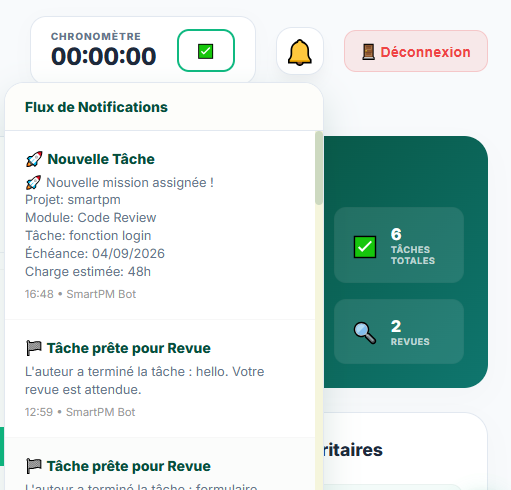
\includegraphics[width=0.8\textwidth]{images/screen_notifications.png}
  \caption{Panneau de notifications en temps r\'eel (WebSocket)}
  \label{fig:scr_notif}
\end{figure}

\begin{figure}[H]
  \centering
  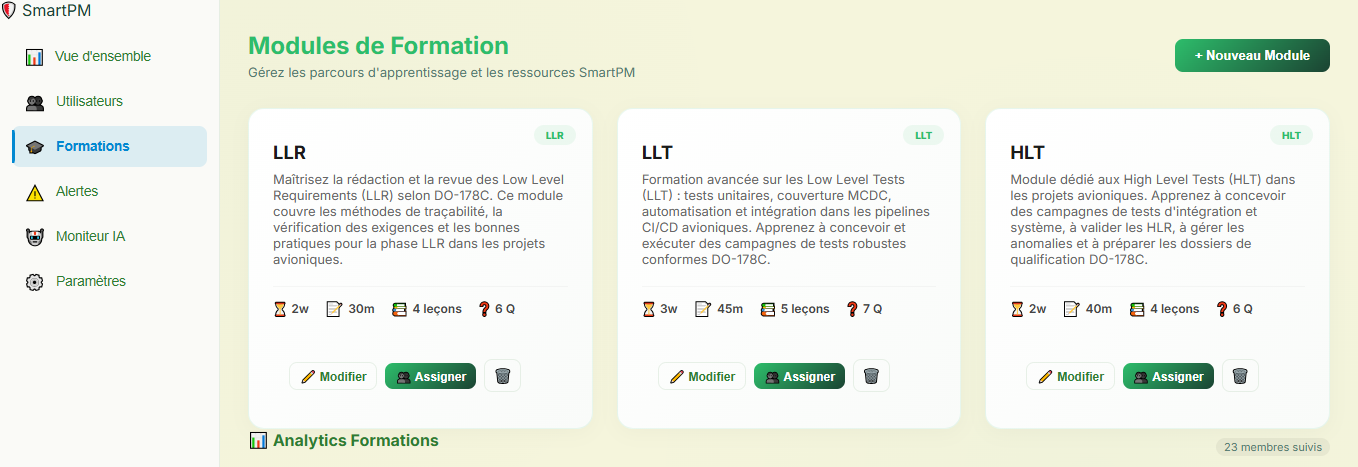
\includegraphics[width=\textwidth]{images/screen_certifications.png}
  \caption{Tableau de certifications par phase DO-178C}
  \label{fig:scr_certif}
\end{figure}

% ─────────────────────────────────────────────────────────
\section*{Conclusion}
% ─────────────────────────────────────────────────────────

Au terme de cette premi\`ere release, les fondations fonctionnelles de
SmartPM sont pleinement op\'erationnelles. Le syst\`eme d'authentification
multi-m\'ethodes garantit la s\'ecurit\'e des acc\`es, la hi\'erarchie de
gestion des projets refl\`ete fid\`element les exigences DO-178C, et les
m\'ecanismes de revues et de notifications assurent une collaboration
fluide et tra\c{c}able entre les membres de l'\'equipe.

\vspace{0.3cm}

Le chapitre suivant pr\'esentera la deuxi\`eme release, qui apporte
l'intelligence artificielle et l'infrastructure DevOps compl\`ete pour
garantir la haute disponibilit\'e de la plateforme.

% ============================================================
%  CHAPITRE 4 — RELEASE 2 : IA, DEVOPS & MONITORING
% ============================================================
\chapter{Release 2 : Intelligence Artificielle, DevOps et Monitoring}

\vspace{-0.3cm}
\begin{tcolorbox}[colback=lightgray, colframe=primaryblue,
  title=\textbf{Plan}, fonttitle=\bfseries]
  \begin{enumerate}[leftmargin=*, label=\arabic*.]
    \item Sprint 4 --- Intelligence Artificielle (AI Assistant)
    \item Sprint 5 --- DevOps, Kubernetes \& Monitoring
  \end{enumerate}
\end{tcolorbox}

% ---------------------------------------------------------
\section*{Introduction}
% ---------------------------------------------------------

La deuxi\`eme release de SmartPM \'el\`eve la plateforme \`a un niveau
industriel en y int\'egrant deux dimensions compl\'ementaires et strat\'egiques.
D'une part, un assistant d'intelligence artificielle contextuel multi-LLM,
capable d'analyser les donn\'ees live des projets et de g\'en\'erer des rapports.
D'autre part, une infrastructure DevOps compl\`ete --- conteneurisation Docker,
orchestration Kubernetes, monitoring Prometheus/Grafana --- garantissant la haute
disponibilit\'e et la scalabilit\'e de la plateforme en production.

\vspace{0.3cm}

Pour chaque sprint, nous pr\'esentons les objectifs, le backlog, les diagrammes
UML (cas d'utilisation, classes, dynamiques) et les interfaces r\'ealis\'ees.

% ═══════════════════════════════════════════════════════════
\newpage
\section{Sprint 4 : Intelligence Artificielle --- AI Assistant}
\label{sec:s4}
% ═══════════════════════════════════════════════════════════

Ce quatri\`eme sprint a pour objectif de doter SmartPM d'un assistant
intelligent capable d'interagir en langage naturel avec les ing\'enieurs
a\'eronautiques et d'analyser les donn\'ees projets en temps r\'eel depuis
MongoDB Atlas.

\subsection{Objectifs du sprint 4}

\begin{itemize}
  \item D\'evelopper un chatbot contextuel aliment\'e par les donn\'ees live
        des projets SmartPM (MongoDB Atlas).
  \item Impl\'ementer une architecture \textbf{Multi-LLM avec fallback automatique} :
        Groq (priorit\'e 1) $\rightarrow$ Gemini (priorit\'e 2)
        $\rightarrow$ OpenRouter (priorit\'e 3).
  \item Cr\'eer un module de simulation de projets (pr\'ediction des risques
        de d\'erive et identification des membres surcharg\'es).
  \item Automatiser la g\'en\'eration de rapports d'avancement structur\'es.
  \item D\'evelopper le panneau \texttt{AiToolsPanel} regroupant tous les outils AI.
  \item Impl\'ementer le module de formations (Training) avec upload et
        indexation de documents de r\'ef\'erence DO-178C.
\end{itemize}

\subsection{Backlog du sprint 4}

\begin{table}[H]
\centering
\renewcommand{\arraystretch}{1.4}
\begin{tabularx}{\textwidth}{|c|X|c|c|}
\hline
\rowcolor{tablehead}
\textcolor{white}{\textbf{ID}} &
\textcolor{white}{\textbf{User Story}} &
\textcolor{white}{\textbf{Priorit\'e}} &
\textcolor{white}{\textbf{Charge (j)}} \\ \hline
US-4.1 & Utilisateur : interagir avec le chatbot AI (donn\'ees live MongoDB) & Haute & 4 \\ \hline
US-4.2 & Syst\`eme : bascule automatique Multi-LLM (Groq$\to$Gemini$\to$OpenRouter) & Haute & 3 \\ \hline
US-4.3 & Manager : simuler un projet (pr\'ediction d\'elais et risques) & Haute & 3 \\ \hline
US-4.4 & Manager : g\'en\'erer un rapport automatique via l'IA & Moyenne & 2 \\ \hline
US-4.5 & Utilisateur : acc\'eder au panneau AiToolsPanel & Moyenne & 2 \\ \hline
US-4.6 & Admin : uploader des documents de formation (Training) & Moyenne & 3 \\ \hline
\end{tabularx}
\caption{Backlog du Sprint 4 --- Intelligence Artificielle}
\label{tab:backlog_s4}
\end{table}

\subsection{Sp\'ecification des besoins fonctionnels}

\subsubsection{Architecture Multi-LLM de SmartPM}

L'une des innovations techniques majeures est l'architecture
\textbf{Multi-LLM avec fallback automatique}. Trois fournisseurs sont
utilis\'es de mani\`ere transparente :

\begin{itemize}
  \item \textbf{Groq} (priorit\'e 1) : fournisseur principal, mod\`ele
        \texttt{llama-3.3-70b-versatile}, latence inf\'erieure \`a 500ms
        pour le premier token.
  \item \textbf{Google Gemini} (priorit\'e 2) : mod\`ele
        \texttt{gemini-1.5-flash}, utilis\'e en cas de d\'epassement de
        quota ou d'indisponibilit\'e de Groq.
  \item \textbf{OpenRouter} (priorit\'e 3) : passerelle vers plusieurs
        mod\`eles (Claude, Mistral) pour garantir la continuit\'e de service.
\end{itemize}

\vspace{0.3cm}

La logique de fallback est impl\'ement\'ee dans \texttt{LlmRouterService}
du microservice FastAPI. En cas d'exception (\texttt{RateLimitError},
\texttt{APIConnectionError}), le service bascule automatiquement vers le
fournisseur suivant dans la cha\^ine de priorit\'e, sans interruption visible
par l'utilisateur.

\subsubsection{Contextualisation des requ\^etes AI}

Avant d'envoyer la requ\^ete au LLM, le backend NestJS enrichit le prompt
avec les informations live du projet : liste des projets actifs et leurs taux
d'avancement, t\^aches en retard, charge de travail de chaque membre,
statistiques des certifications, revues en attente depuis plus de 48 heures.
Ce contexte injecte dans le \textit{system prompt} permet \`a l'assistant
de r\'epondre \`a des questions comme \textit{<< Quels sont les projets
\`a risque cette semaine ? >>} avec des donn\'ees pr\'ecises et actualis\'ees.

\subsubsection{Diagramme de cas d'utilisation}

\begin{figure}[H]
  \centering
  \includegraphics[width=\textwidth]{figures/chapter4/sprint4/uc_sprint4.png}
  \caption{Diagramme de cas d'utilisation --- Sprint 4 (AI Assistant)}
  \label{fig:uc_s4}
\end{figure}

\subsection{Diagramme de classes du sprint 4}

\begin{figure}[H]
  \centering
  \includegraphics[width=\textwidth]{figures/chapter4/sprint4/class_sprint4.png}
  \caption{Diagramme de classes --- Sprint 4 (AI Assistant)}
  \label{fig:class_s4}
\end{figure}

\subsection{Diagrammes dynamiques du sprint 4}

\subsubsection{Diagramme de s\'equence --- Chatbot AI en streaming SSE}

Le diagramme~\ref{fig:seq_chat} d\'etaille le flux complet d'une interaction
avec le chatbot SmartPM. L'utilisation des \textit{Server-Sent Events} (SSE)
permet d'afficher la r\'eponse token par token, offrant une exp\'erience
utilisateur similaire \`a ChatGPT.

\vspace{0.3cm}

Le flux se d\'eroule en quatre \'etapes :
(1)~L'utilisateur envoie un message depuis \texttt{AiChatbotComponent} ;
(2)~le \texttt{AiIntegrationService} NestJS collecte le contexte live depuis
MongoDB Atlas ;
(3)~la requ\^ete enrichie est transmise au microservice FastAPI qui appelle
le LLM s\'electionn\'e ;
(4)~les tokens sont relay\'es en streaming SSE vers le client Angular.

\begin{figure}[H]
  \centering
  \includegraphics[width=\textwidth]{figures/chapter4/sprint4/seq_chatbot.png}
  \caption{Diagramme de s\'equence --- Chatbot AI avec streaming SSE}
  \label{fig:seq_chat}
\end{figure}

\subsubsection{Diagramme d'activit\'e --- Logique de fallback Multi-LLM}

\begin{figure}[H]
  \centering
  \includegraphics[width=\textwidth]{figures/chapter4/sprint4/activity_llm_fallback.png}
  \caption{Diagramme d'activit\'e --- Strat\'egie Multi-LLM avec fallback}
  \label{fig:act_llm}
\end{figure}

\subsection{R\'ealisation du sprint 4}

Le module \texttt{AiIntegrationModule} NestJS joue le r\^ole de passerelle
entre Angular et le microservice FastAPI. Le microservice IA est d\'evelopp\'e
en \textbf{Python 3.11} avec \textbf{FastAPI} et la biblioth\`eque
\textbf{LangChain} pour abstraire les appels aux diff\'erents LLMs.
Il expose trois endpoints : \texttt{POST /chat/stream} (chatbot streaming),
\texttt{POST /simulate} (simulation projet) et \texttt{POST /report}
(g\'en\'eration rapport).

\begin{figure}[H]
  \centering
  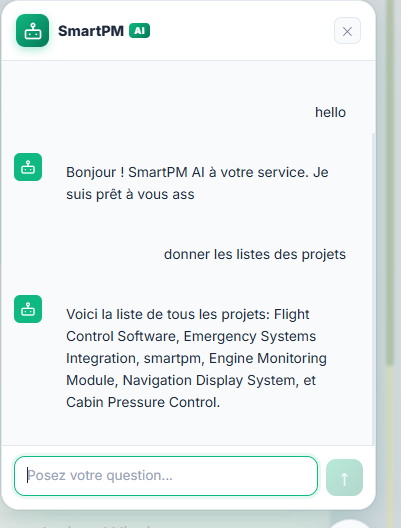
\includegraphics[width=\textwidth]{images/screen_chatbot.png}
  \caption{Interface du chatbot AI contextuel de SmartPM}
  \label{fig:scr_chat}
\end{figure}

\begin{figure}[H]
  \centering
  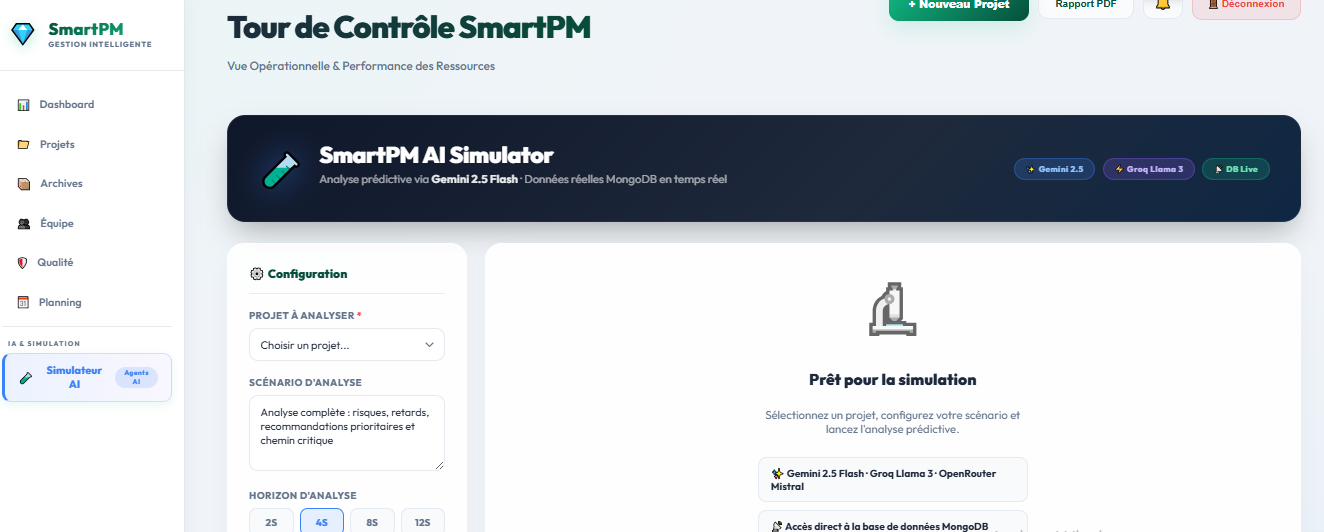
\includegraphics[width=\textwidth]{images/screen_ai_tools.png}
  \caption{AiToolsPanel --- Panneau centralis\'e des outils IA}
  \label{fig:scr_tools}
\end{figure}

\begin{figure}[H]
  \centering
  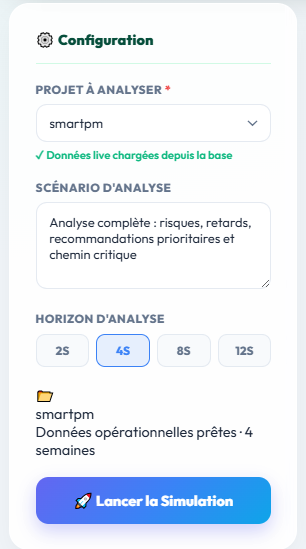
\includegraphics[width=\textwidth]{images/screen_simulation.png}
  \caption{Module de simulation --- Pr\'ediction des risques par l'IA}
  \label{fig:scr_sim}
\end{figure}

\begin{figure}[H]
  \centering
  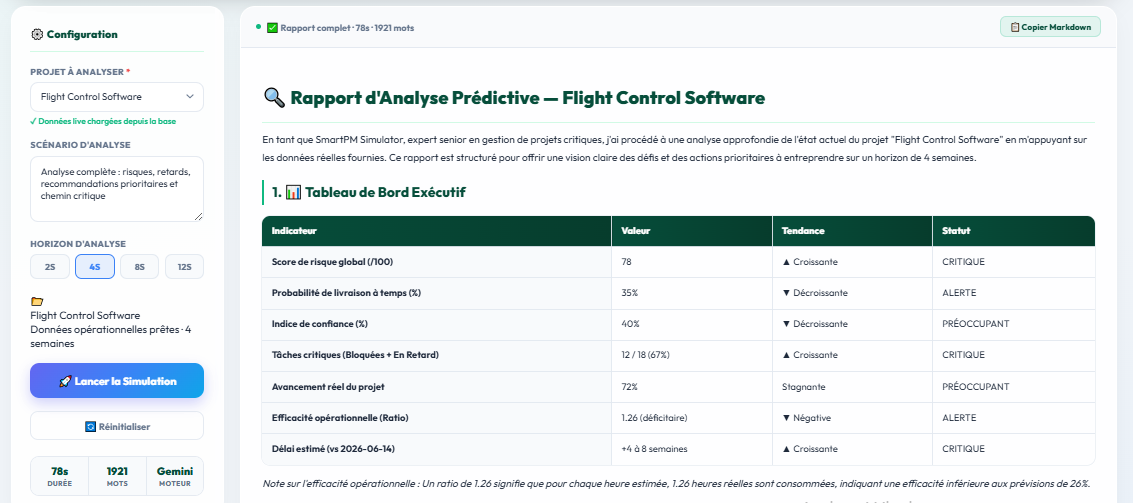
\includegraphics[width=\textwidth]{images/screen_report.png}
  \caption{G\'en\'eration automatique de rapport d'avancement via l'IA}
  \label{fig:scr_report}
\end{figure}

\begin{figure}[H]
  \centering
  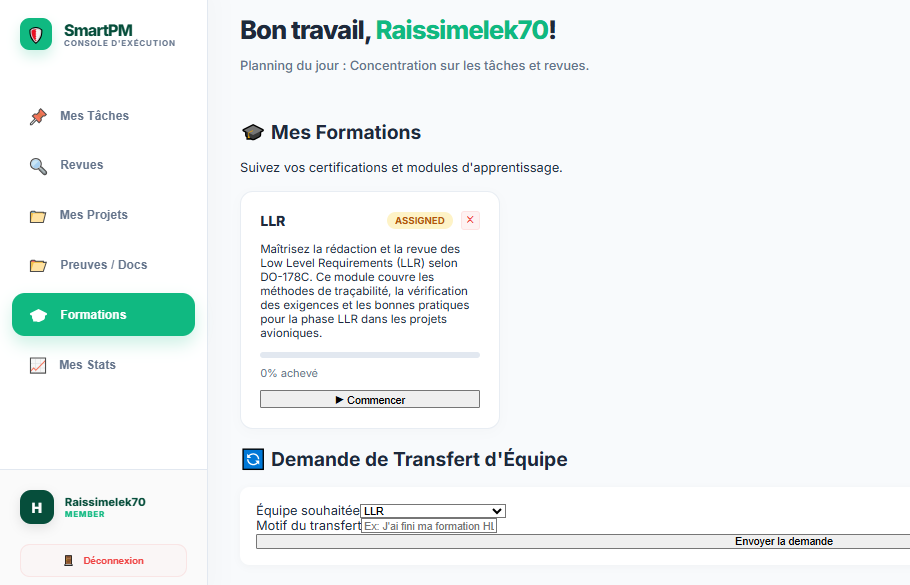
\includegraphics[width=\textwidth]{images/screen_training.png}
  \caption{Module Training --- Gestion des documents de r\'ef\'erence DO-178C}
  \label{fig:scr_train}
\end{figure}

% ═══════════════════════════════════════════════════════════
\newpage
\section{Sprint 5 : DevOps, Kubernetes \& Monitoring}
\label{sec:s5}
% ═══════════════════════════════════════════════════════════

Ce cinqui\`eme et dernier sprint industrialise le d\'eploiement de SmartPM
en le dotant d'une infrastructure de production robuste, automatis\'ee et
observable. Il s'articule autour de trois axes : \textbf{conteneurisation}
Docker, \textbf{orchestration} Kubernetes et \textbf{monitoring}
Prometheus/Grafana.

\subsection{Objectifs du sprint 5}

\begin{itemize}
  \item Cr\'eer des \texttt{Dockerfile} optimis\'es (multi-stage) pour les
        trois services : frontend Angular, backend NestJS, service AI FastAPI.
  \item \'Ecrire les manifestes Kubernetes YAML pour les six deployments.
  \item Configurer Prometheus (endpoint \texttt{/metrics}) et Grafana
        (dashboards pr\'econfig\'ur\'es).
  \item S\'ecuriser le backend avec Helmet, ThrottlerGuard (100~req/min/IP)
        et une politique CORS stricte.
  \item Impl\'ementer le \texttt{BackupReplicationService} MongoDB Atlas.
  \item Automatiser le d\'eploiement via le script \texttt{start-devops.bat}.
\end{itemize}

\subsection{Backlog du sprint 5}

\begin{table}[H]
\centering
\renewcommand{\arraystretch}{1.4}
\begin{tabularx}{\textwidth}{|c|X|c|c|}
\hline
\rowcolor{tablehead}
\textcolor{white}{\textbf{ID}} &
\textcolor{white}{\textbf{User Story}} &
\textcolor{white}{\textbf{Priorit\'e}} &
\textcolor{white}{\textbf{Charge (j)}} \\ \hline
US-5.1 & Dockerfile optimis\'e pour les 3 services (frontend, backend, AI) & Haute & 2 \\ \hline
US-5.2 & Manifestes K8s : 6 Deployments + Services (NodePort) & Haute & 3 \\ \hline
US-5.3 & Prometheus : collecte m\'etriques API NestJS (\texttt{/metrics}) & Haute & 2 \\ \hline
US-5.4 & Grafana : dashboards m\'etriques API et \'etat des pods & Haute & 2 \\ \hline
US-5.5 & S\'ecurit\'e backend : Helmet + ThrottlerGuard + CORS strict & Haute & 1 \\ \hline
US-5.6 & BackupReplicationService MongoDB Atlas & Moyenne & 2 \\ \hline
US-5.7 & Script CI/CD automatis\'e : start-devops.bat & Moyenne & 1 \\ \hline
\end{tabularx}
\caption{Backlog du Sprint 5 --- DevOps, Kubernetes \& Monitoring}
\label{tab:backlog_s5}
\end{table}

\subsection{Sp\'ecification des besoins fonctionnels}

\subsubsection{Diagramme de cas d'utilisation}

\begin{figure}[H]
  \centering
  \includegraphics[width=\textwidth]{figures/chapter4/sprint5/uc_sprint5.png}
  \caption{Diagramme de cas d'utilisation --- Sprint 5 (DevOps \& Monitoring)}
  \label{fig:uc_s5}
\end{figure}

\subsection{Diagramme de classes du sprint 5}

L'infrastructure DevOps ne g\'en\`ere pas d'entit\'es de donn\'ees \`a
proprement parler. Les principaux artefacts sont les configurations
Kubernetes (Deployment, Service, ConfigMap, PersistentVolumeClaim) et les
tableaux de bord Grafana. Le tableau~\ref{tab:k8s_pods} r\'ecapitule les
composants d\'eploy\'es.

\begin{table}[H]
\centering
\renewcommand{\arraystretch}{1.4}
\begin{tabularx}{\textwidth}{|l|l|c|c|}
\hline
\rowcolor{tablehead}
\textcolor{white}{\textbf{Deployment}} &
\textcolor{white}{\textbf{Image Docker}} &
\textcolor{white}{\textbf{Replicas}} &
\textcolor{white}{\textbf{NodePort}} \\ \hline
frontend   & smartpm/frontend:latest   & 2 & 30080 \\ \hline
backend    & smartpm/backend:latest    & 2 & 30000 \\ \hline
ai-service & smartpm/ai:latest         & 1 & 30800 \\ \hline
prometheus & prom/prometheus:latest    & 1 & 30090 \\ \hline
grafana    & grafana/grafana:latest    & 1 & 30300 \\ \hline
mongo      & MongoDB Atlas (Cloud)     & --- & --- \\ \hline
\end{tabularx}
\caption{R\'ecapitulatif des Deployments Kubernetes de SmartPM}
\label{tab:k8s_pods}
\end{table}

\subsection{Diagrammes dynamiques du sprint 5}

\subsubsection{Architecture de d\'eploiement Kubernetes}

\begin{figure}[H]
  \centering
  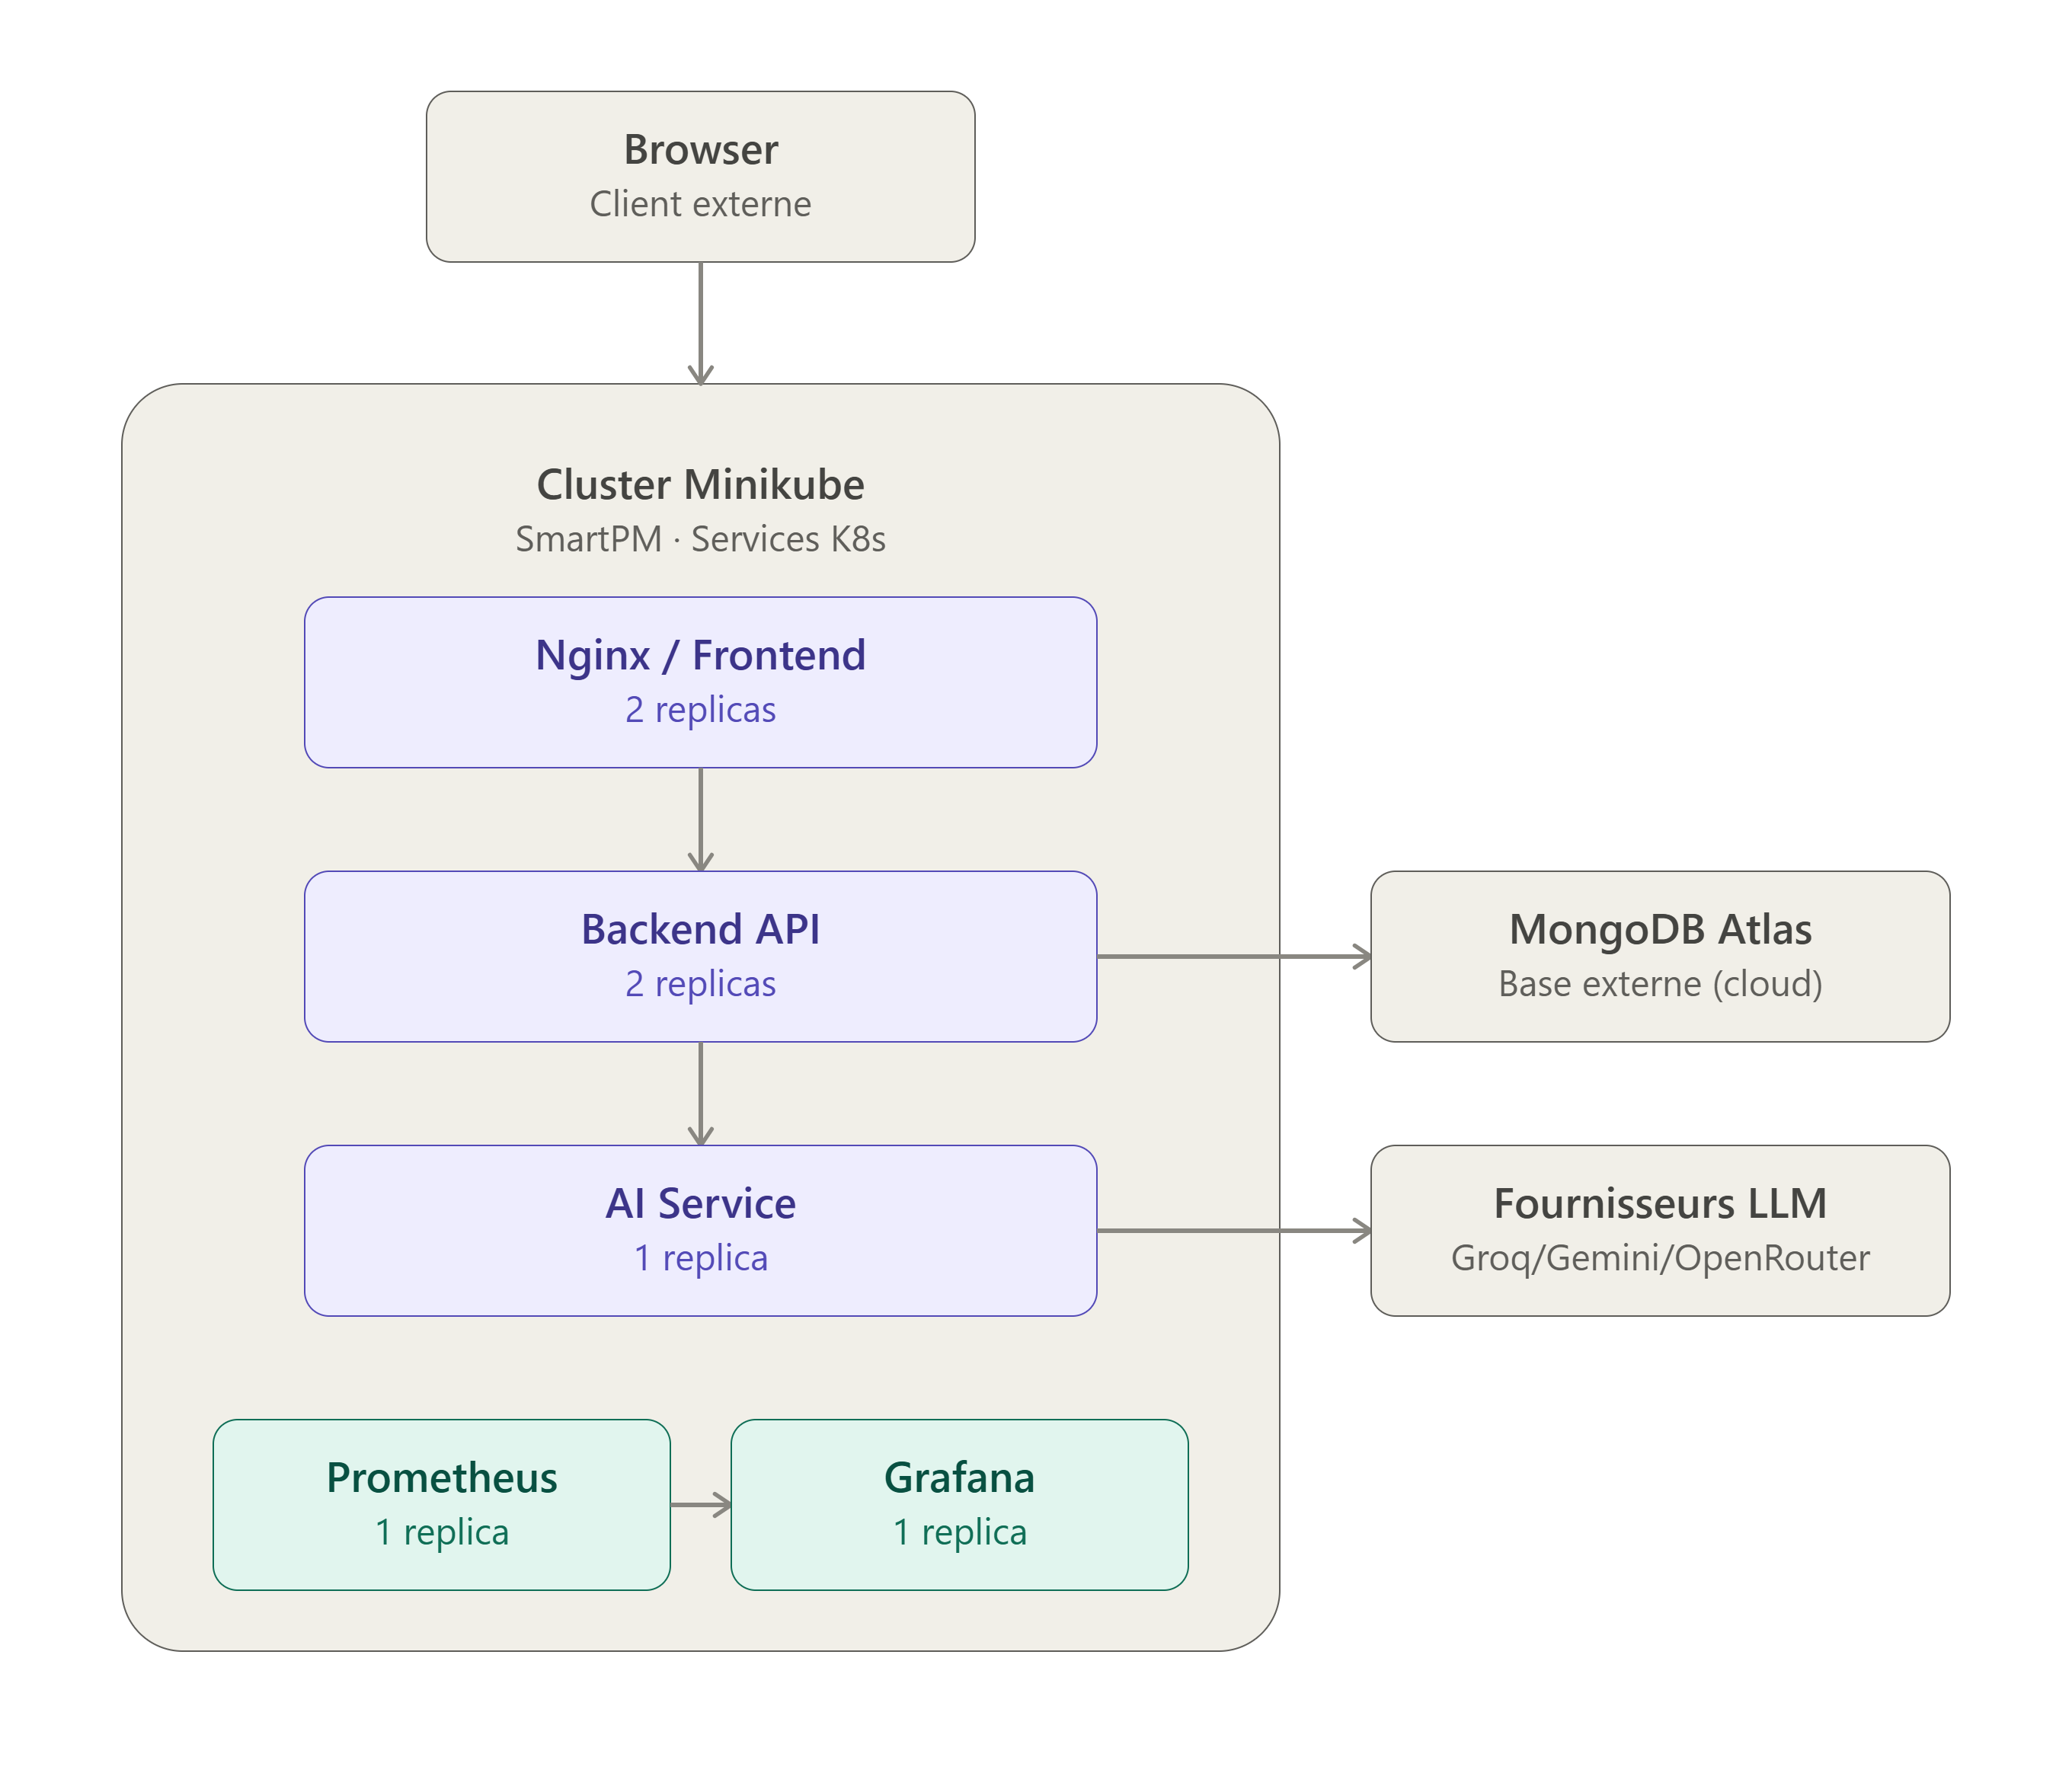
\includegraphics[width=\textwidth]{images/arch_k8s.png}
  \caption{Architecture de d\'eploiement Kubernetes de SmartPM}
  \label{fig:arch_k8s}
\end{figure}

\subsubsection{Diagramme de s\'equence --- Pipeline CI/CD}

Le script \texttt{start-devops.bat} automatise six \'etapes s\'equentielles :
(1)~v\'erification Minikube, (2)~\texttt{docker build} des trois images,
(3)~\texttt{minikube image load}, (4)~\texttt{kubectl apply -f k8s/},
(5)~attente que tous les pods soient \texttt{Running}, (6)~affichage
des URLs d'acc\`es.

\begin{figure}[H]
  \centering
  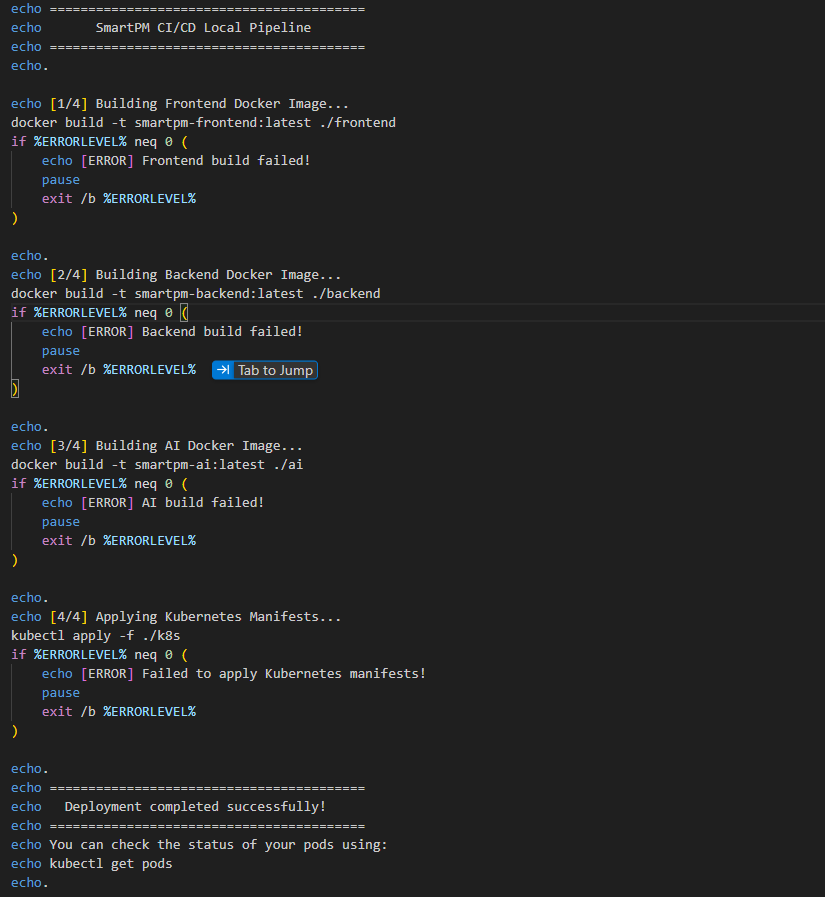
\includegraphics[width=\textwidth]{images/pipeline_cicd.png}
  \caption{Pipeline CI/CD automatis\'e --- \texttt{start-devops.bat}}
  \label{fig:pipeline}
\end{figure}

\subsection{R\'ealisation du sprint 5}

\subsubsection{Conteneurisation Docker}

Les trois services sont conteneuris\'es avec des Dockerfiles optimis\'es :
\textbf{Frontend} en build multi-stage (\texttt{node:20-alpine} pour la
compilation Angular + \texttt{nginx:alpine} pour le service, image finale
$<$50\,MB) ;
\textbf{Backend NestJS} bas\'e sur \texttt{node:20-alpine} avec
\texttt{npm ci --only=production} ;
\textbf{Service AI} bas\'e sur \texttt{python:3.11-slim} avec
\texttt{uvicorn main:app --host 0.0.0.0 --port 8000}.

\subsubsection{S\'ecurisation multi-couches du backend}

Trois couches de s\'ecurit\'e compl\'ementaires ont \'et\'e ajout\'ees :
\textbf{Helmet} (en-t\^etes HTTP : \texttt{X-Frame-Options: DENY},
\texttt{Content-Security-Policy}, \texttt{Strict-Transport-Security}),
\textbf{ThrottlerGuard} (100 requ\^etes/minute/IP, anti-DDoS et
anti-brute-force) et \textbf{CORS strict} (origines autoris\'ees via
\texttt{ALLOWED\_ORIGINS}).

\subsubsection{Monitoring Prometheus \& Grafana}

Le module \texttt{@willsoto/nestjs-prometheus} expose l'endpoint
\texttt{GET /metrics} en format Prometheus, collectant :
\texttt{http\_request\_duration\_seconds} (histogramme de latence par route),
\texttt{http\_requests\_total} (compteur par statut HTTP),
\texttt{nodejs\_heap\_size\_used\_bytes} (m\'emoire heap) et
\texttt{process\_cpu\_seconds\_total} (CPU).

\vspace{0.3cm}

Deux dashboards Grafana sont pr\'econfig\'ur\'es via ConfigMap Kubernetes :
\textbf{Dashboard API SmartPM} (requ\^etes/minute, latence P95, taux d'erreurs)
et \textbf{Dashboard Infrastructure} (\'etat des pods, CPU, m\'emoire).

\subsubsection{Interfaces r\'ealis\'ees}

\begin{figure}[H]
  \centering
  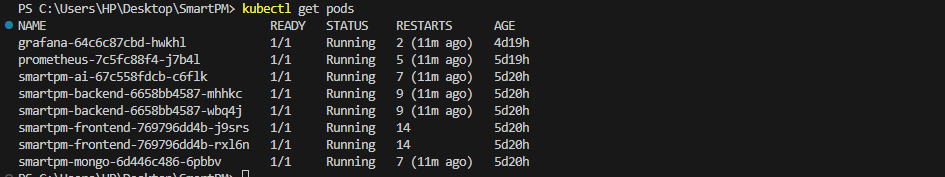
\includegraphics[width=\textwidth]{images/screen_kubectl_pods.png}
  \caption{\'Etat des pods Kubernetes --- \texttt{kubectl get pods}}
  \label{fig:scr_k8s}
\end{figure}

\begin{figure}[H]
  \centering
  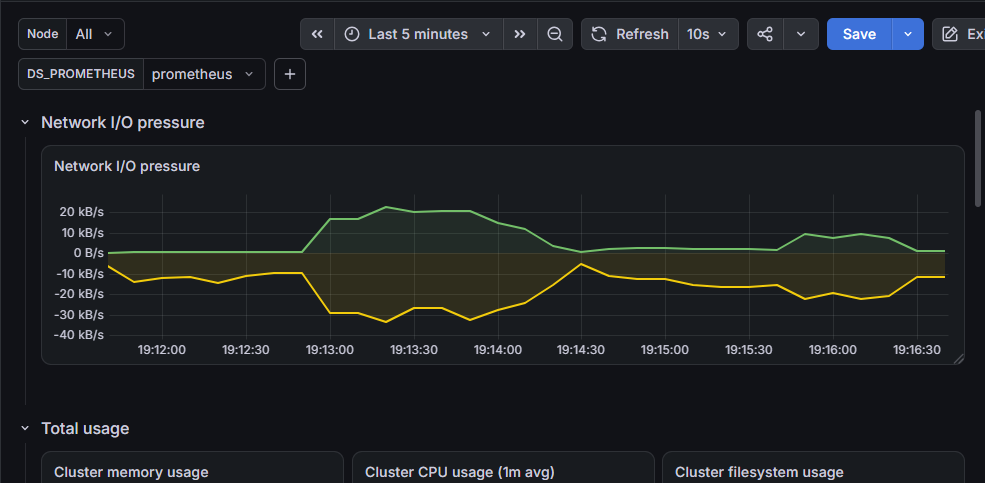
\includegraphics[width=\textwidth]{images/screen_grafana.png}
  \caption{Dashboard Grafana --- M\'etriques API de SmartPM}
  \label{fig:scr_grafana}
\end{figure}

\begin{figure}[H]
  \centering
  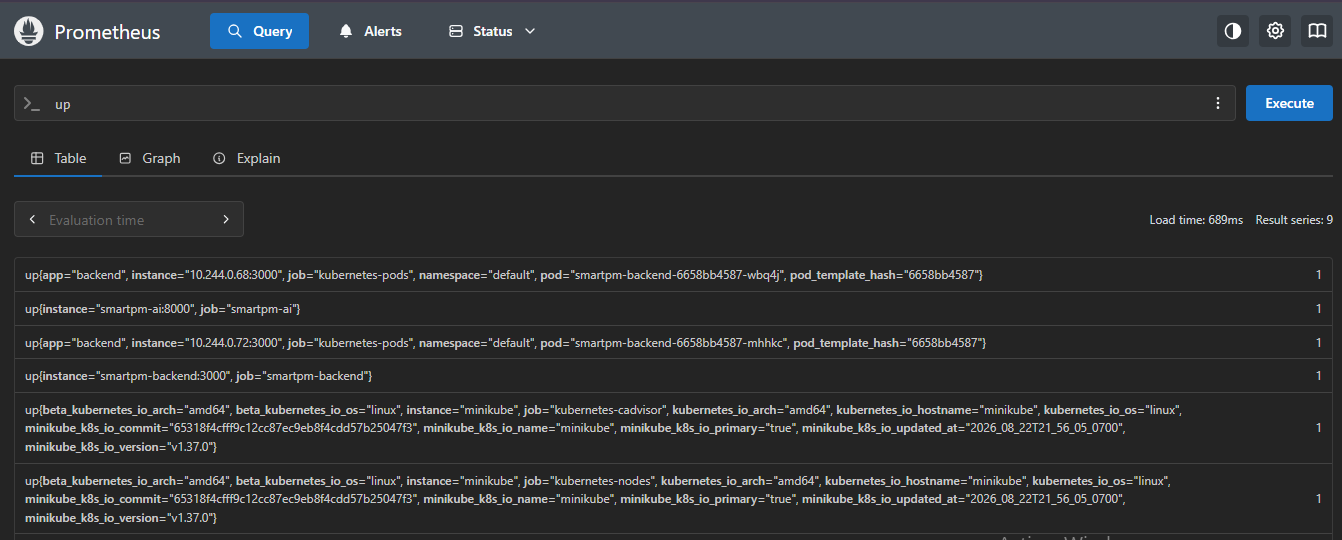
\includegraphics[width=\textwidth]{images/screen_prometheus.png}
  \caption{Interface Prometheus --- Supervision des m\'etriques}
  \label{fig:scr_prom}
\end{figure}

\begin{figure}[H]
  \centering
  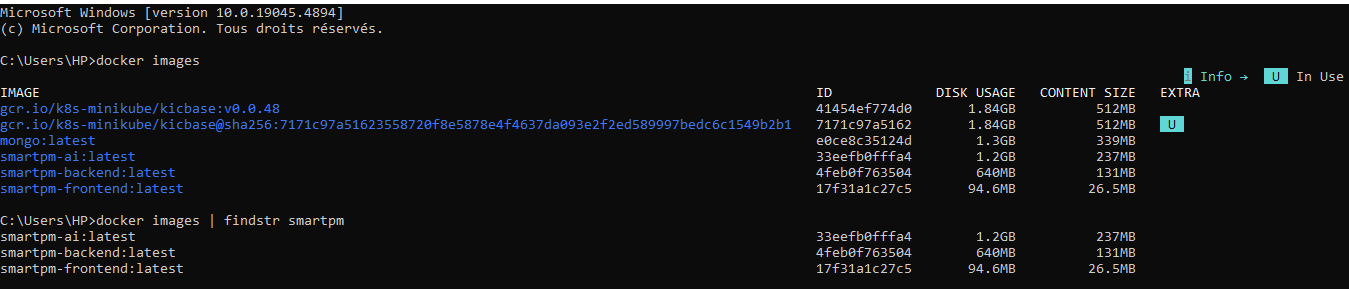
\includegraphics[width=\textwidth]{images/screen_docker_images.png}
  \caption{Images Docker construites pour SmartPM}
  \label{fig:scr_docker}
\end{figure}

% ---------------------------------------------------------
\section*{Conclusion}
% ---------------------------------------------------------

La deuxi\`eme release marque l'aboutissement technique du projet SmartPM.
L'int\'egration d'un assistant AI contextuel multi-LLM avec streaming SSE
apporte une valeur ajout\'ee significative et diff\'erenciante pour les
ing\'enieurs a\'eronautiques, en leur offrant une assistance intelligente
nourrie des donn\'ees r\'eelles de leurs projets.

\vspace{0.3cm}

L'infrastructure Kubernetes d\'eploy\'ee garantit la scalabilit\'e, la
r\'esilience et la tra\c{c}abilit\'e compl\`ete des services en production.
Le monitoring Prometheus/Grafana assure une observabilit\'e en temps r\'eel,
indispensable dans un contexte industriel o\`u la disponibilit\'e est critique.

\vspace{0.3cm}

La plateforme SmartPM est d\'esormais op\'erationnelle, s\'ecuris\'ee et
monitor\'ee, pr\^ete \`a \'evoluer vers une int\'egration compl\`ete dans
les cha\^ines d'outillage de certification DO-178C de niveau DAL-A.

% ============================================================
%  CONCLUSION GÉNÉRALE
% ============================================================
\chapter*{Conclusion g\'en\'erale}
\addcontentsline{toc}{chapter}{Conclusion g\'en\'erale}
\markboth{Conclusion g\'en\'erale}{}
\vspace{0.3cm}

Ce Projet de Fin d'\'Etudes, r\'ealis\'e pour le compte de Capgemini au sein de Capgemini Tunisie, marque l'aboutissement de mon cursus d'ing\'enieur \`a Tek-Up et repr\'esente une mise en pratique concr\`ete des comp\'etences techniques et m\'ethodologiques acquises durant ma formation.

Inscrit au c\oe ur de la modernisation de la gestion des projets a\'eronautiques dans un contexte de conformit\'e \`a la norme DO-178C, ce travail visait \`a optimiser un processus de suivi et de r\'evision de code historiquement manuel et complexe. La plateforme SmartPM r\'epond \`a cet enjeu en rationalisant l'ensemble de la cha\^ine op\'erationnelle et en apportant un cadre unifi\'e, automatis\'e et collaboratif pour la coordination entre les d\'eveloppeurs, les relecteurs et les managers.

Le projet a \'et\'e men\'e selon une approche agile Scrum, structur\'ee autour de deux releases compl\'ementaires :
\begin{itemize}
  \item Release 1 : mise en place du socle fonctionnel (authentification s\'ecuris\'ee, gestion de la hi\'erarchie des projets, cr\'eation et suivi des t\^aches et des revues techniques) ;
  \item Release 2 : automatisation de l'assistance contextuelle par l'IA (RAG multi-LLM) et introduction d'une infrastructure DevOps compl\`ete (Kubernetes, Monitoring) pour le pilotage op\'erationnel.
\end{itemize}

Cette d\'emarche a abouti \`a des r\'esultats tangibles : diminution des t\^aches manuelles, meilleure synchronisation entre acteurs, fiabilisation du suivi des revues techniques et mise \`a disposition d'indicateurs de performance permettant un pilotage \'eclair\'e du processus. La plateforme offre d\'esormais une base technique robuste, con\c{c}ue pour \'evoluer et s'adapter \`a de futurs besoins.

Au-del\`a des aspects techniques, ce projet a \'et\'e une exp\'erience humaine enrichissante, m\^elant collaboration, compr\'ehension fine des enjeux m\'etiers et rigueur dans la conception logicielle. Il m'a permis de consolider mes comp\'etences en architecture logicielle, en int\'egration de syst\`emes et en pratiques DevOps, tout en d\'ecouvrant les r\'ealit\'es op\'erationnelles d'un grand groupe.

Les perspectives d'\'evolution de SmartPM sont nombreuses : \'elargissement \`a de nouveaux cas d'usage, int\'egration d'algorithmes d'automatisation plus avanc\'es, am\'elioration de l'exp\'erience utilisateur et exploration de nouveaux indicateurs de pilotage.

Au final, SmartPM constitue aujourd'hui un socle solide et \'evolutif qui modernise un maillon essentiel de l'ing\'enierie logicielle a\'eronautique. Ce projet contribue directement \`a l'am\'elioration de la performance op\'erationnelle et, \`a terme, \`a une meilleure garantie de s\'ecurit\'e et de conformit\'e pour les clients de Capgemini.


% Webographie
% ============================================================
%  WEBOGRAPHIE (Format manuel identique à l'exemple)
% ============================================================
\chapter*{Webographie}
\addcontentsline{toc}{chapter}{Webographie}
\markboth{Webographie}{}

\begin{enumerate}[label={[\arabic*]}, leftmargin=0.8cm, itemsep=0.3cm]
  \item \og Capgemini - NOTRE ENTREPRISE, \fg{} visit\'e le 7 f\'evrier 2026. adresse : \url{https://www.capgemini.com/fr-fr/notre-groupe/qui-sommes-nous/}
  \item \og Certification DO-178C : l'avanc\'ee des normes a\'eronautiques en 2026 ? \fg{} Visit\'e le 12 f\'evrier 2026. adresse : \url{https://www.rtca.org/do-178c}
  \item \og M\'ethodes agiles : une belle d\'efinition, \fg{} visit\'e le 20 mars 2026. adresse : \url{https://www.qualitystreet.fr/2007/11/20/methodes-agiles-un-belle-definition/}
  \item \og La m\'ethode Scrum et ses b\'en\'efices, \fg{} visit\'e le 25 mars 2026. adresse : \url{https://www.bocasay.com/fr/methode-scrum-benefices-developpements-web/}
  \item \og Qu'est-ce que le langage UML, \fg{} visit\'e le 10 avril 2026. adresse : \url{https://www.lucidchart.com/pages/fr/langage-uml}
  \item \og Comprendre l'architecture des Microservices, \fg{} visit\'e le 15 avril 2026. adresse : \url{https://code-garage.com/blog/comprendre-l-architecture-microservices}
  \item \og Architecture avec NestJS, \fg{} visit\'e le 18 avril 2026. adresse : \url{https://docs.nestjs.com/first-steps}
  \item \og Qu'est-ce que le RAG, \fg{} visit\'e le 5 mai 2026. adresse : \url{https://dev.to/sambhavyadavtech/what-is-retrieval-augmented-generation-rag-236j}
  \item \og Pr\'esentation du VSCode, \fg{} visit\'e le 10 mai 2026. adresse : \url{https://code.visualstudio.com/docs}
  \item \og Angular - \'Ecosyst\`eme Frontend de Google, \fg{} visit\'e le 15 mai 2026. adresse : \url{https://angular.dev/overview}
  \item \og Le tutoriel Python, \fg{} visit\'e le 20 mai 2026. adresse : \url{https://docs.python.org/fr/3/tutorial/}
  \item \og MongoDB Atlas en bref, \fg{} visit\'e le 25 mai 2026. adresse : \url{https://www.mongodb.com/fr-fr/atlas}
  \item \og Exploration des Capacit\'es des mod\`eles LLM Llama 3.1, \fg{} visit\'e le 5 juin 2026. adresse : \url{https://groq.com/llama-3-1/}
  \item \og Qu'est-ce que FastAPI, \fg{} visit\'e le 10 juin 2026. adresse : \url{https://fastapi.tiangolo.com/}
\end{enumerate}

\newpage
\section*{Webographie Sprint 5}
\markboth{Webographie}{}

\begin{enumerate}[label={[\arabic*]}, leftmargin=0.8cm, itemsep=0.3cm, start=15]
  \item \og Pipeline DevOps, \fg{} visit\'e le 15 juin 2026. adresse : \url{https://www.atlassian.com/fr/devops/devops-tools/devops-pipeline}
  \item \og Qu'est-ce que Kubernetes, l'orchestrateur de conteneurs ? \fg{} Visit\'e le 20 juin 2026. adresse : \url{https://kubernetes.io/fr/docs/concepts/overview/what-is-kubernetes/}
  \item \og Qu'est-ce que Docker ? Notre guide complet, \fg{} visit\'e le 25 juin 2026. adresse : \url{https://about.gitlab.com/fr-fr/blog/what-is-docker-comprehensive-guide/}
  \item \og Prometheus - La solution pour votre monitoring, \fg{} visit\'e le 1 juillet 2026. adresse : \url{https://prometheus.io/docs/introduction/overview/}
  \item \og Visualisation de m\'etriques \`a l'aide de Grafana, \fg{} visit\'e le 5 juillet 2026. adresse : \url{https://grafana.com/docs/grafana/latest/introduction/}
  \item \og Minikube : tout savoir sur la plateforme Kubernetes locale, \fg{} visit\'e le 10 juillet 2026. adresse : \url{https://minikube.sigs.k8s.io/docs/start/}
\end{enumerate}


% ============================================================
%  RÉSUMÉ ET ABSTRACT (Séparés sur 2 pages selon la demande)
% ============================================================
\newpage
\thispagestyle{empty}
\vspace*{1cm}

\begin{center}
\textbf{\Large R\'esum\'e}
\end{center}
\vspace{0.4cm}

Ce rapport synth\'etise le travail r\'ealis\'e dans le cadre du projet de fin d'\'etudes pour l'obtention du dipl\^ome national d'ing\'enieur en informatique, men\'e au sein de \og Capgemini Tunisie \fg{} pour le compte d'un client a\'eronautique. Il porte sur la modernisation de la gestion des projets et des revues techniques, n\'ecessaires lorsqu'un d\'eveloppement logiciel exige une certification DO-178C. Jusqu'alors, le processus reposait sur des \'echanges dispers\'es et manuels. Il a \'et\'e repens\'e gr\^ace \`a la mise en place de SmartPM, une plateforme web interne unifi\'ee.

SmartPM simplifie la planification des t\^aches, automatise une partie des revues avec un assistant IA, et assure un suivi clair et centralis\'e des certifications. L'objectif est d'optimiser la coordination entre acteurs, de r\'eduire les d\'elais de traitement et d'am\'eliorer durablement la qualit\'e de service au sein du cycle de d\'eveloppement critique.

\vspace{0.4cm}
\noindent\textbf{Mots cl\'es :} Gestion de projet, A\'eronautique, Scrum, Plateforme web, DO-178C, DevOps, RAG, LLM

\newpage
\thispagestyle{empty}
\vspace*{1cm}

\begin{center}
\textbf{\Large Abstract}
\end{center}
\vspace{0.4cm}

This report summarizes the end-of-studies project carried out at ``Capgemini Tunisia'' on behalf of an aeronautical client. It focuses on modernizing the management of projects and technical reviews, required when software development demands DO-178C certification. Previously, the process relied on manual and fragmented exchanges. It has been redesigned through the implementation of SmartPM, a unified internal web platform.

SmartPM streamlines task scheduling, automates part of the reviews with an AI assistant, and provides clear, centralized tracking of certifications. Its goal is to enhance coordination between stakeholders, reduce processing times, and sustainably improve service quality within the critical development lifecycle.

\vspace{0.4cm}
\noindent\textbf{Keywords :} Project Management, Aeronautics, Scrum, Web Platform, DO-178C, DevOps, RAG, LLM

\vspace*{\fill}

% --- Footer Capgemini ---
\noindent\rule{\textwidth}{1pt}
\begin{center}
\textbf{Capgemini Tunisie}\\
Parc Technologique El Ghazala Bloc N$^\circ$3, Route de Raoued Km 3.5, 2088 Ariana, Tunisie \\
T\'el\'ephone : +216 31 378 800
\end{center}


\end{document}
